\section{Results} \label{sec:results}
Several simulations were run with \gls{sispo} in order to assess the capabilities and quality of the output of the three stages, i.e. rendering, compression and reconstruction. Furthermore, the effects of compression using the \gls{jp2} standard on the quality of \gls{3d} model reconstruction.

\subsection{Rendering} \label{sec:results_sim}
A subset of all settings was kept constant for all simulations. The instrument settings are presented in Table~\ref{tab:inst_settings} and the settings for the \gls{sssb} in Table~\ref{tab:sssb_settings}. The specific values were chosen in order to mimic the scenario in~\cite{Pajusalu2019CharacterizationMapping}.

\begin{table}[htb]
    \centering
    \caption{Instrument Settings}
    \label{tab:inst_settings}
    \begin{tabular}{l|l}
        \textbf{Parameter Name} & \textbf{Value} \\ \hline
        res       & $\SI{2464}{} \times \SI{2054}{}$   \\
        pix\_l        & \SI{3.45}{\micro\meter}     \\
        focal\_l       & \SI{230}{\milli\meter}     \\
        aperture\_d     &  \SI{4}{\centi\meter} \\
        wavelength  & \SI{550}{\nano\meter} \\
        quantum\_eff & \SI{0.25}{} \\
        color\_depth & \SI{8}{\bit}
    \end{tabular}
\end{table}

\begin{table}[htb]
    \centering
    \caption{\gls{sssb} settings.}
    \label{tab:sssb_settings}
    \begin{tabular}{l|l}
        \textbf{Parameter Name} & \textbf{Value} \\ \hline
        a       & \SI{1.644641475071416}{\astronomicalunit}   \\
        e        & \SI{3.838774437558215E-01}{}\\
        i       & \SI{3.408231185574551E+00}{\radian}\\
        P &  \SI{7.703805051391988E+02}{\radian} \\
        omega  & \SI{3.192958853076784E+02}{\radian} \\
        Omega & \SI{7.320940216397703E+01}{\radian} \\
        M & \SI{1.967164895190036E+02}{\radian} \\
        date & 2017-08-19T00:00:00.000 \\
        rotation\_rate & \SI{8133.48}{\per\second} \\
        albedo & \SI{0.15}{} \\
        max\_dim & \SI{512}{}
    \end{tabular}
\end{table}

\begin{table}[htb]
    \centering
    \caption{Simulation settings.}
    \label{tab:sim_settings}
    \begin{tabular}{l|l}
        \textbf{Parameter Name} & \textbf{Value} \\ \hline
        duration       & \SI{120}{\second}   \\
        encounter\_date & 2017-08-15T12:00:00.000\\
        frames       & \SI{120}{}     \\
        relative\_velocity     &  \SI{10}{\kilo\meter\per\second} \\
        with\_terminator  & \SI{0}{} \\
        with\_sunnyside & \SI{1}{} \\
        timesampler\_mode & \SI{1}{} \\
        exposure & \SI{0}{} \\
        samples & \SI{48}{} \\
        device & \gls{gpu} \\
        tile\_size & \SI{512}{} \\
        with\_clipping & \SI{1}{}
    \end{tabular}
\end{table}

\subsubsection{Image Comparison}
In a first step, the overall image quality is compared visually to real images. A set of images at different distances of nuclei with different sizes is depicted in Figure~\ref{fig:render_quali_comparison}. A set of five images from asteroid Bennu taken by the PolyCam aboard the \textit{OSIRIS-REx} mission is shown in Figure~\ref{fig:render_quali_bennu}. Additionally, the rendered images are compared to images of comet \gls{67p} taken by the OSIRIS imager aboard the \textit{Rosetta} spacecraft. Figure~\ref{fig:render_quali_67p} shows one image that represents all important features of \gls{67p}. A collection of several views of the comet \gls{81p}, also known as Wild 2, are shown in Figure~\ref{fig:render_quali_81p}. \Gls{81p} was visited during the \textit{Stardust} mission~\cite{Brownlee2003Stardust:Mission}.

\begin{figure}[htb]
    \centering
        \begin{subfigure}[b]{0.48\textwidth}
            \centering
                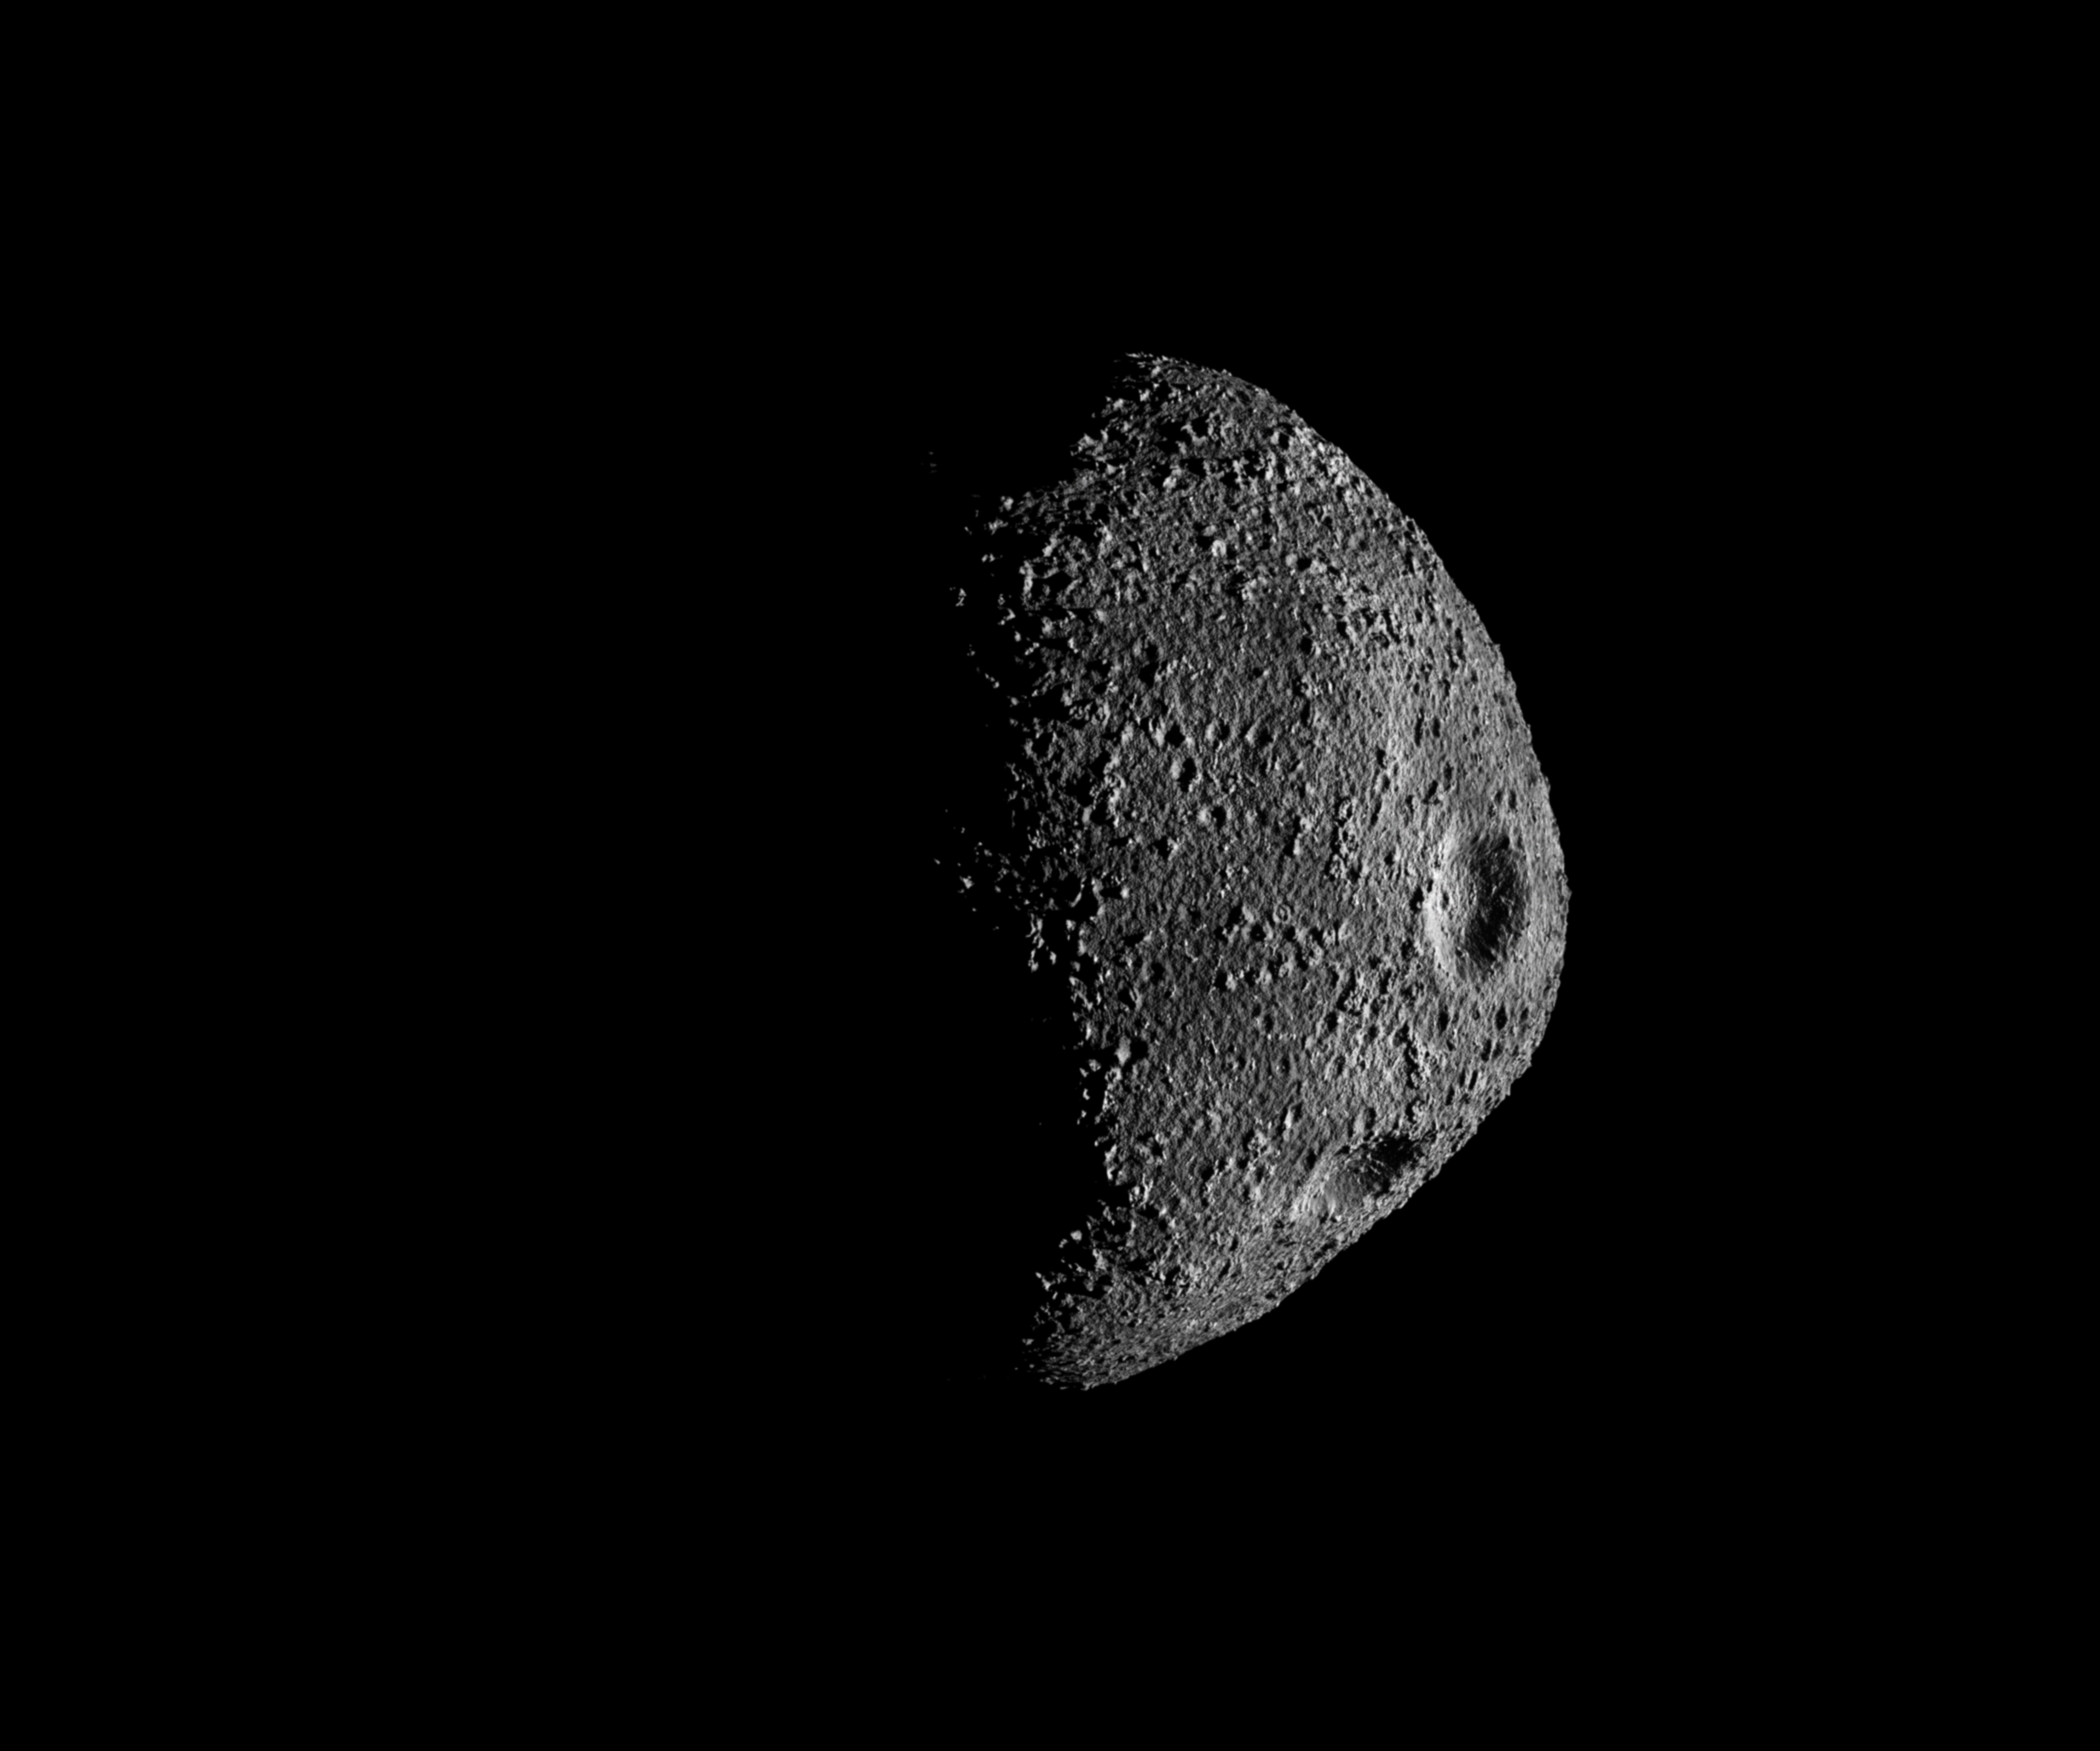
\includegraphics[width=\textwidth]{doc/thesis/0_figures/procedural_terrain/50_10_Inst_2017-08-15T115755-845000.png}
            \caption{\SI{566}{\kilo\meter}.}
            \label{fig:render_quali_comparison_1}
        \end{subfigure}
        \\
        \begin{subfigure}[b]{0.48\textwidth}
            \centering
                \includegraphics[width=\textwidth]{doc/thesis/0_figures/procedural_terrain/50_10_Inst_2017-08-15T115855-260000.png}
            \caption{\SI{106}{\kilo\meter}.}
            \label{fig:render_quali_comparison_2}
        \end{subfigure}
    \caption{Surface of a \SI{10}{\kilo\meter} \gls{sssb} at the given distances.}
    \label{fig:render_quali_comparison}
\end{figure}

\begin{figure}[htb]
    \centering
    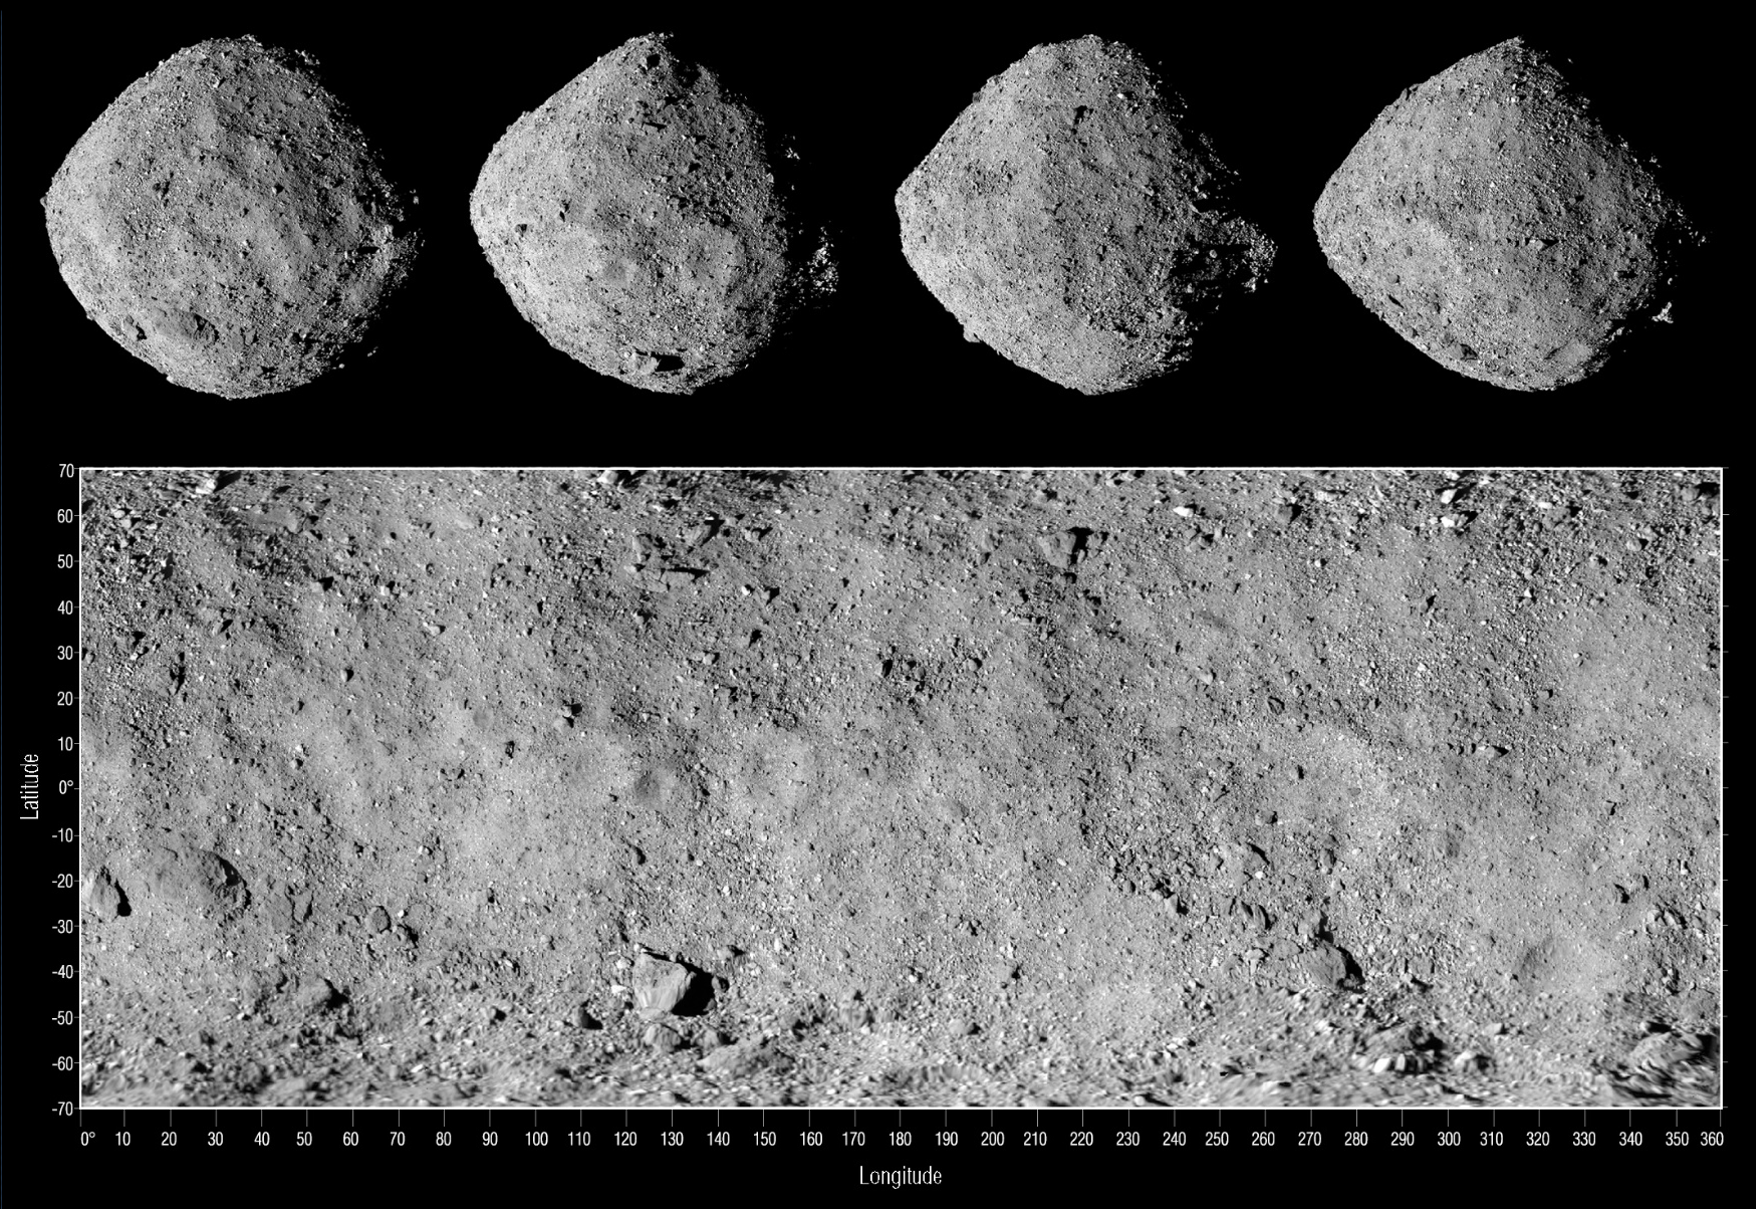
\includegraphics[width=.7\textwidth]{doc/thesis/0_figures/procedural_terrain/2963_Bennu.png}
    \caption{Four images of asteroid Bennu and a global surface mosaic. These images were taken by the PolyCam aboard the \textit{OSIRIS-REx} mission~\cite{FourExploration}.}
    \label{fig:render_quali_bennu}
\end{figure}

\begin{figure}[htb]
    \centering
    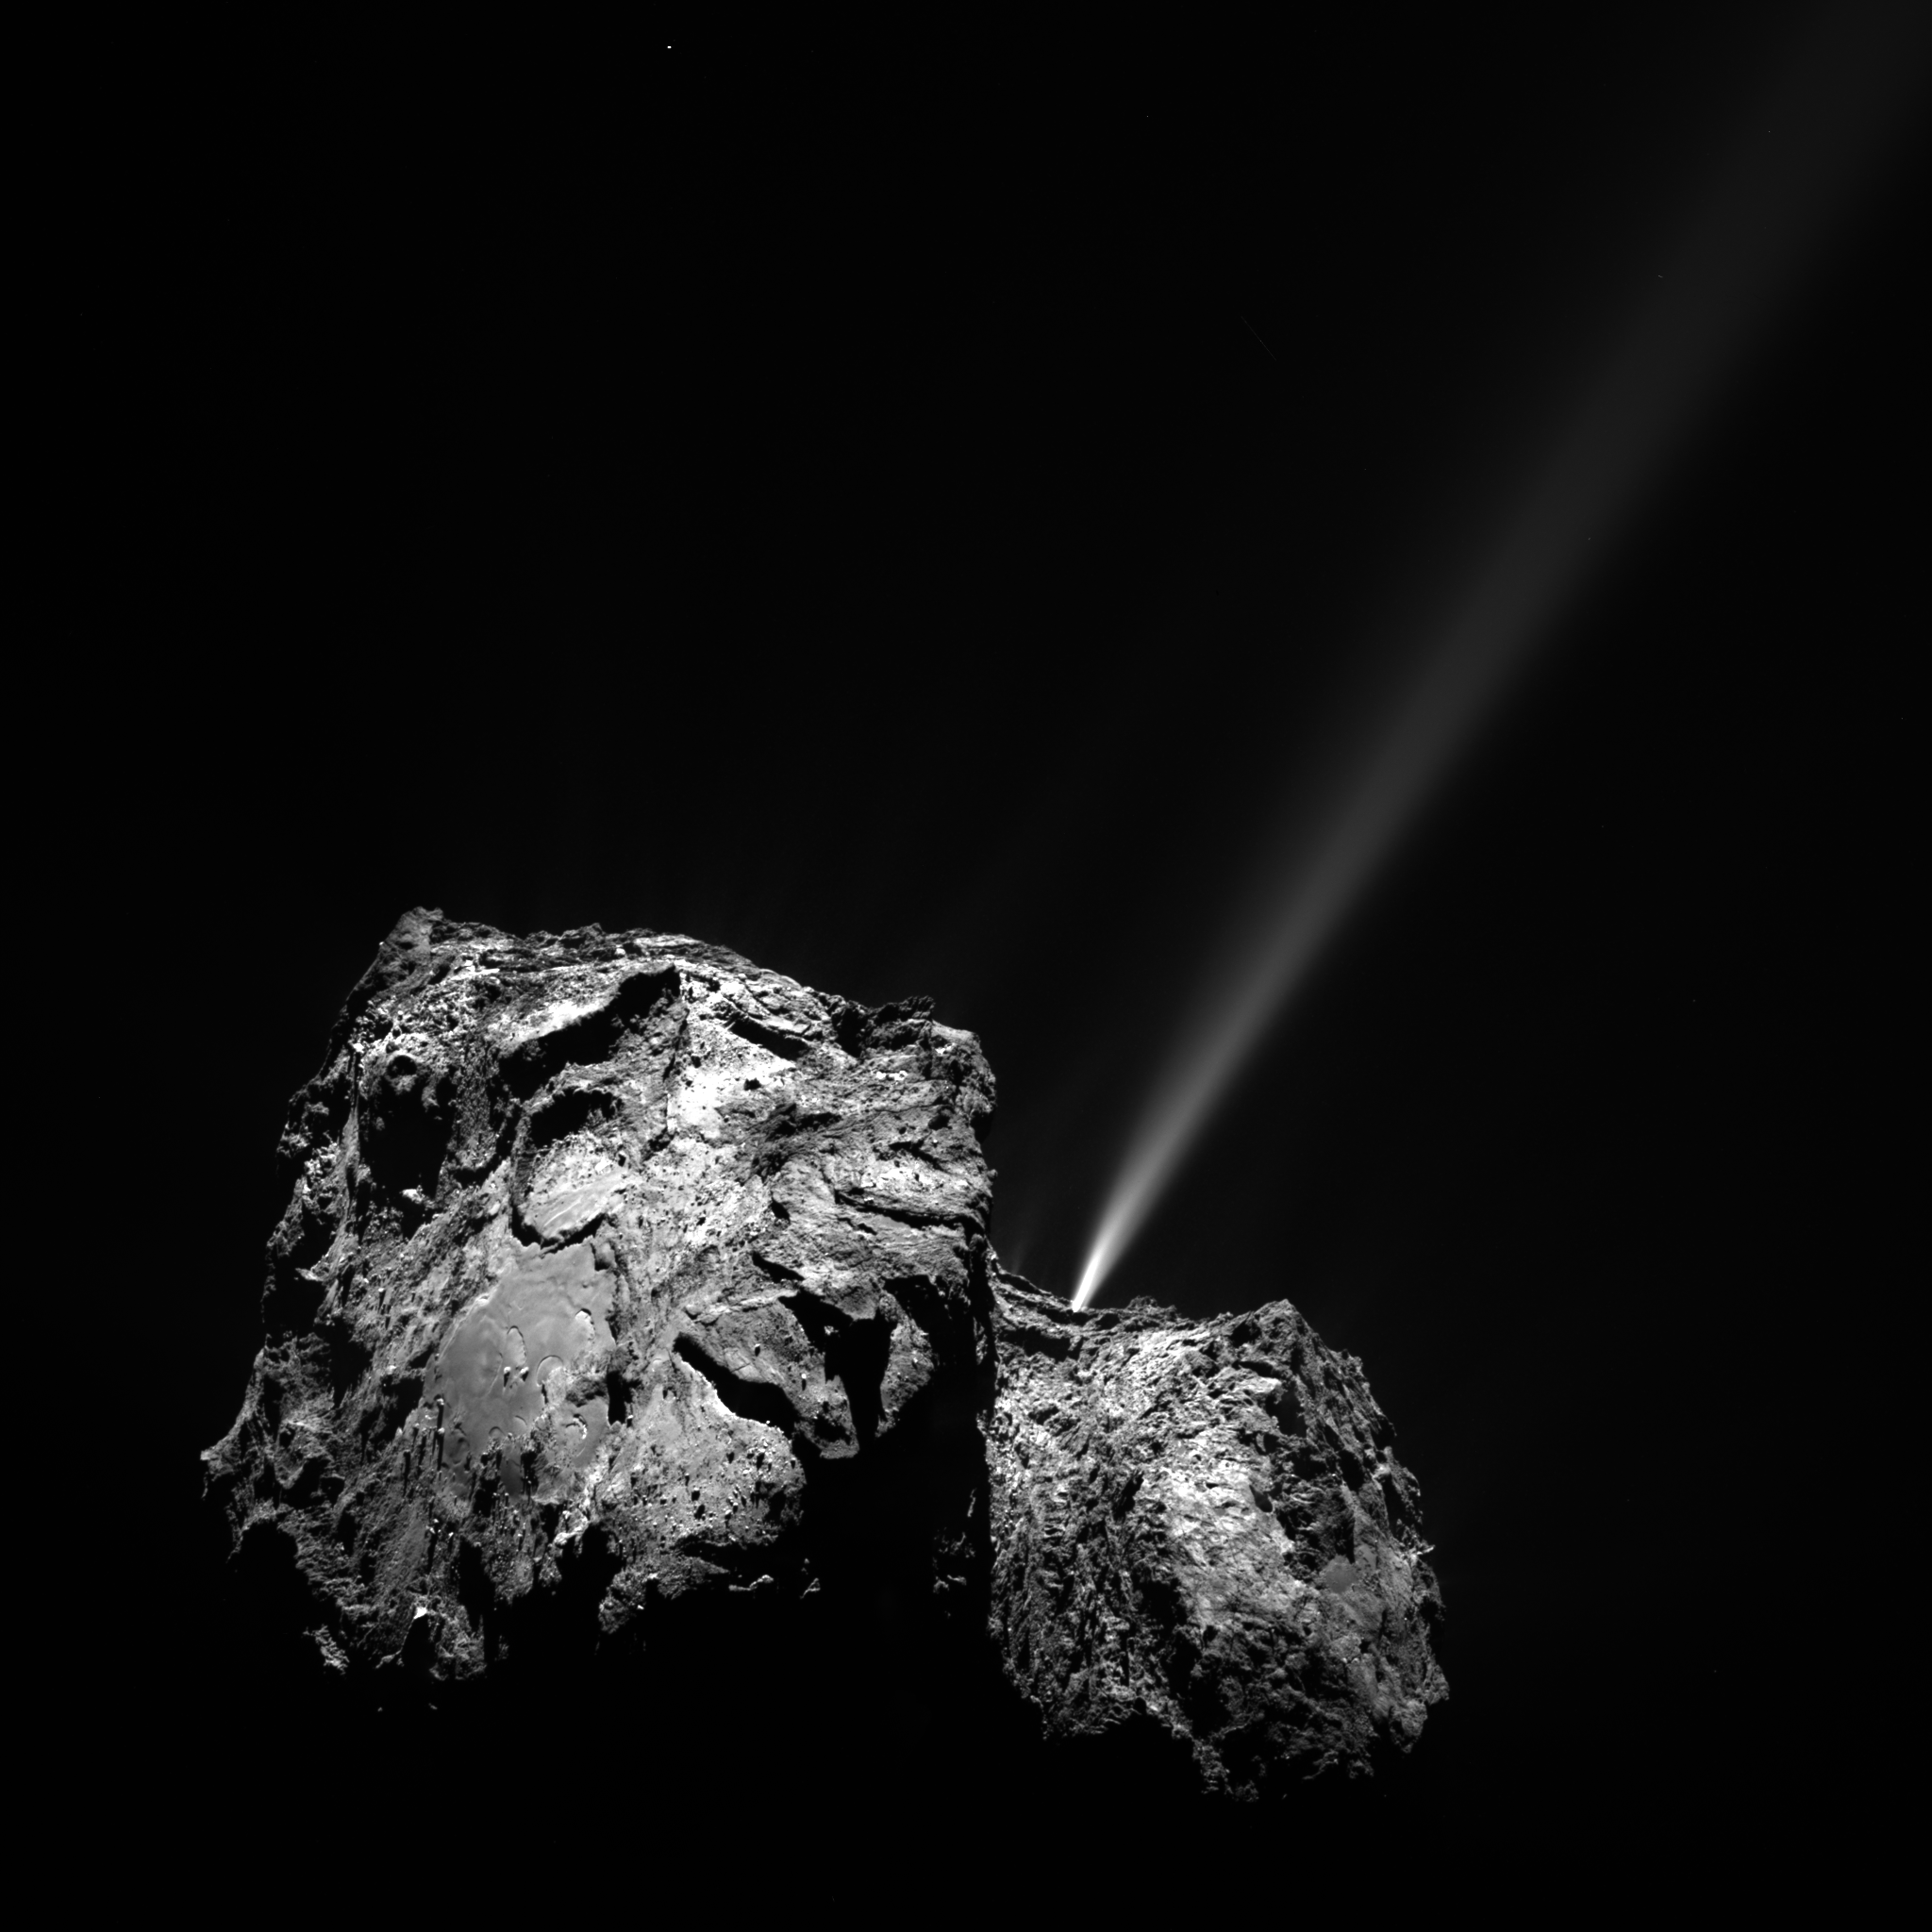
\includegraphics[width=.8\textwidth]{doc/thesis/0_figures/procedural_terrain/67P_CG.PNG}
    \caption{Representative image of comet \acrlong{67p}. This image was taken by the OSIRIS imager aboard the \textit{Rosetta} mission~\cite{OSIRISArchiveb}}.
    \label{fig:render_quali_67p}
\end{figure}

\begin{figure}[htb]
    \centering
    \includegraphics[width=.7\textwidth]{doc/thesis/0_figures/procedural_terrain/Wild2.jpg}
    \caption{Collection of images of comet \acrlong{81p} taken during the \textit{Stardust} mission by its navigation camera~\cite{StardustImages}.}
    \label{fig:render_quali_81p}
\end{figure}

While all images exhibit show pits, the overall appearance of the rendered images resembles the smoother pits of Bennu better than the sharper pits of \gls{67p} or \gls{81p}. The overall looks of the rendered images resemble the real images of Bennu well. The rocks and boulders present on Bennu's surface are also visible in the rendered images. When comparing the rendered images to the image of \gls{67p} or \gls{81p}, the most pronounced difference are the jets. \Gls{sispo} does not contain a gas and dust model that would produce a coma or jets and therefore these are missing in the rendered images. While the surface of both comets also feature some rocks and boulders, it is more defined by ridge-like structures. This type of feature is missing in the rendered images. Hence, the rendering output of \gls{sispo} better represents asteroids than comets.

\subsubsection{Different Distances}
Through procedural terrain generation, \gls{sispo} produces results for a large range of encounter distances. Example images with different surface distances and \gls{sssb} sizes are shown in Figure~\ref{fig:img_procedural_10k}.

\begin{figure}[htb]
    \centering
        \begin{subfigure}[b]{0.75\textwidth}
            \centering
            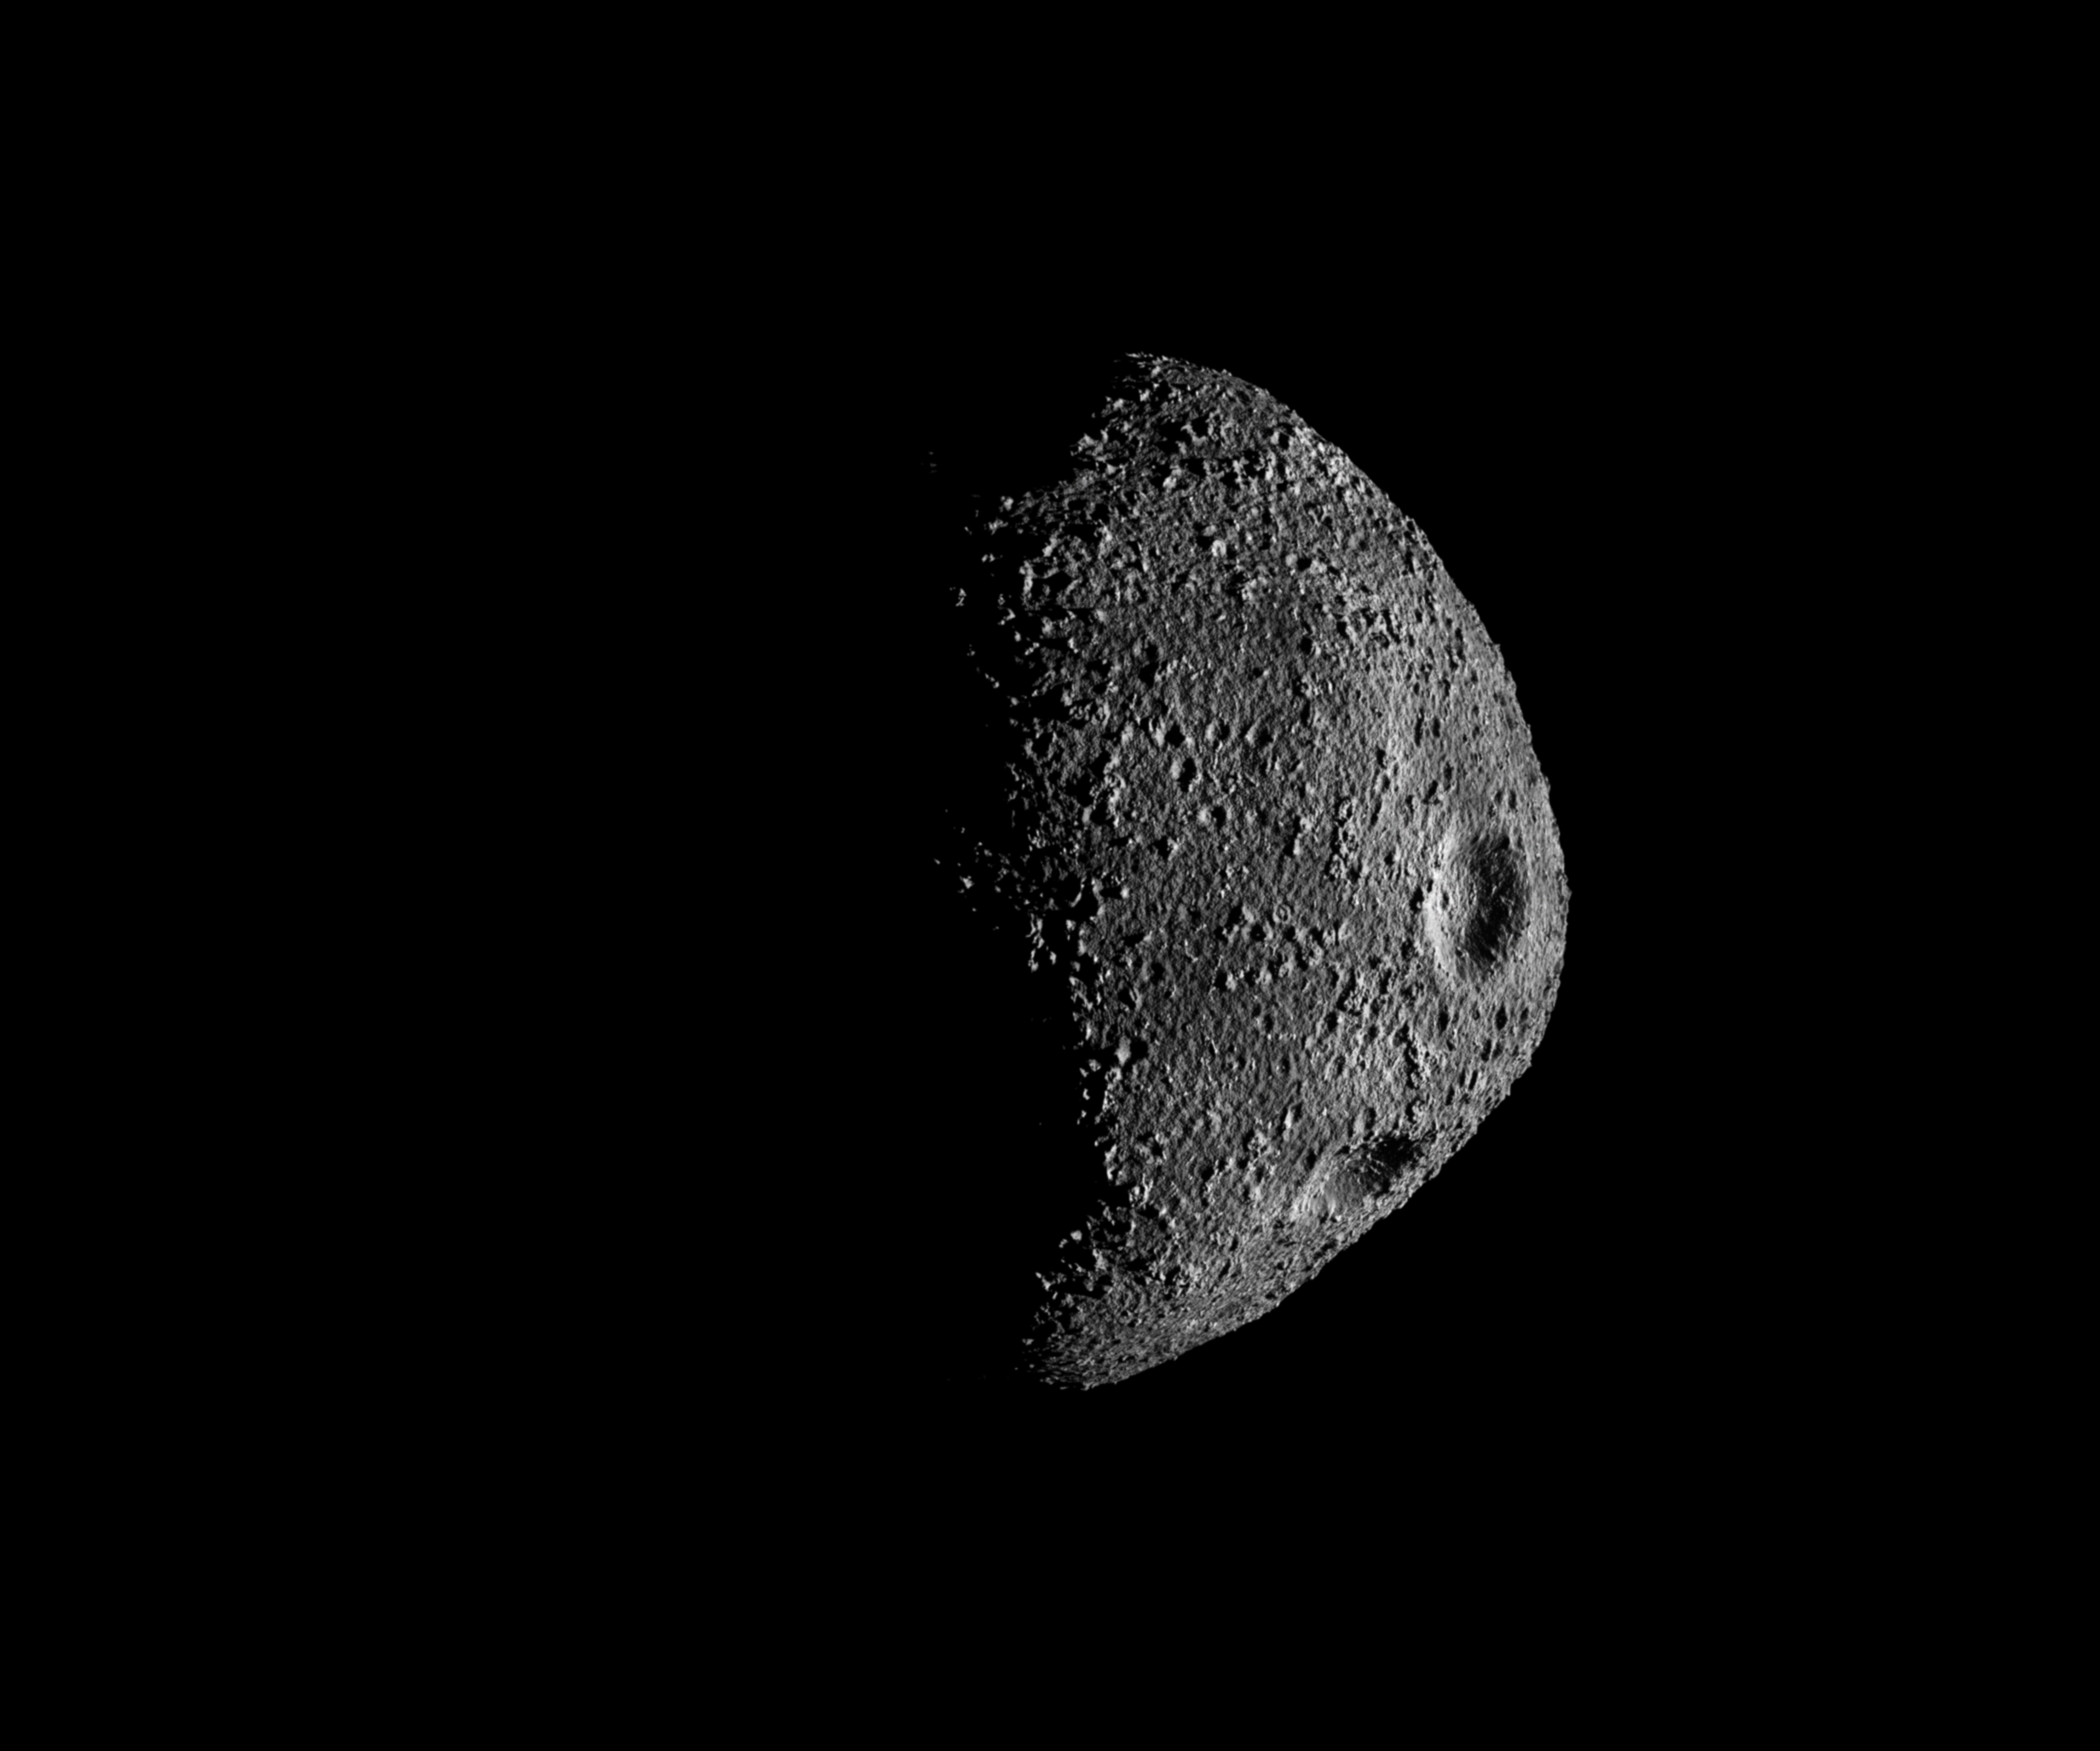
\includegraphics[width=\textwidth]{doc/thesis/0_figures/procedural_terrain/50_10_Inst_2017-08-15T115755-845000.png}
            \caption{\SI{566}{\kilo\meter}.}
            \label{fig:img_procedural_500}
        \end{subfigure}
        \\
        \begin{subfigure}[b]{0.75\textwidth}
            \centering
            \includegraphics[width=\textwidth]{doc/thesis/0_figures/procedural_terrain/50_10_Inst_2017-08-15T115855-260000.png}
            \caption{\SI{106}{\kilo\meter}.}
            \label{fig:img_procedural_100}
        \end{subfigure}
    \caption{Surface of a \SI{10}{\kilo\meter} \gls{sssb} at the given distances.}
    \label{fig:img_procedural_10k}
\end{figure}

It is visible from Figure~\ref{fig:img_procedural_10k} that surface features and details do not degrade visually. Moving closer to the surface reveals more details, such as tiny bumps between larger structures which are not visible from larger distances. The visible quality of surface features is defined by the shader implementation. 

\subsubsection{Composition}
The composition process uses raw images rendered with Blender and produces photometrically calibrated images. An example set of four images consisting of two images before and after calibration is shown in Figure~\ref{fig:composition_before_after}. All four images were converted to \SI{8}{\bit} images. Two effects can be seen. First, the original images differ in there overall brightness. This difference is removed by the calibration. Secondly, images become brighter by the calibration process. 

\begin{figure}[htb]
    \centering
        \begin{subfigure}[b]{0.48\textwidth}
            \centering
                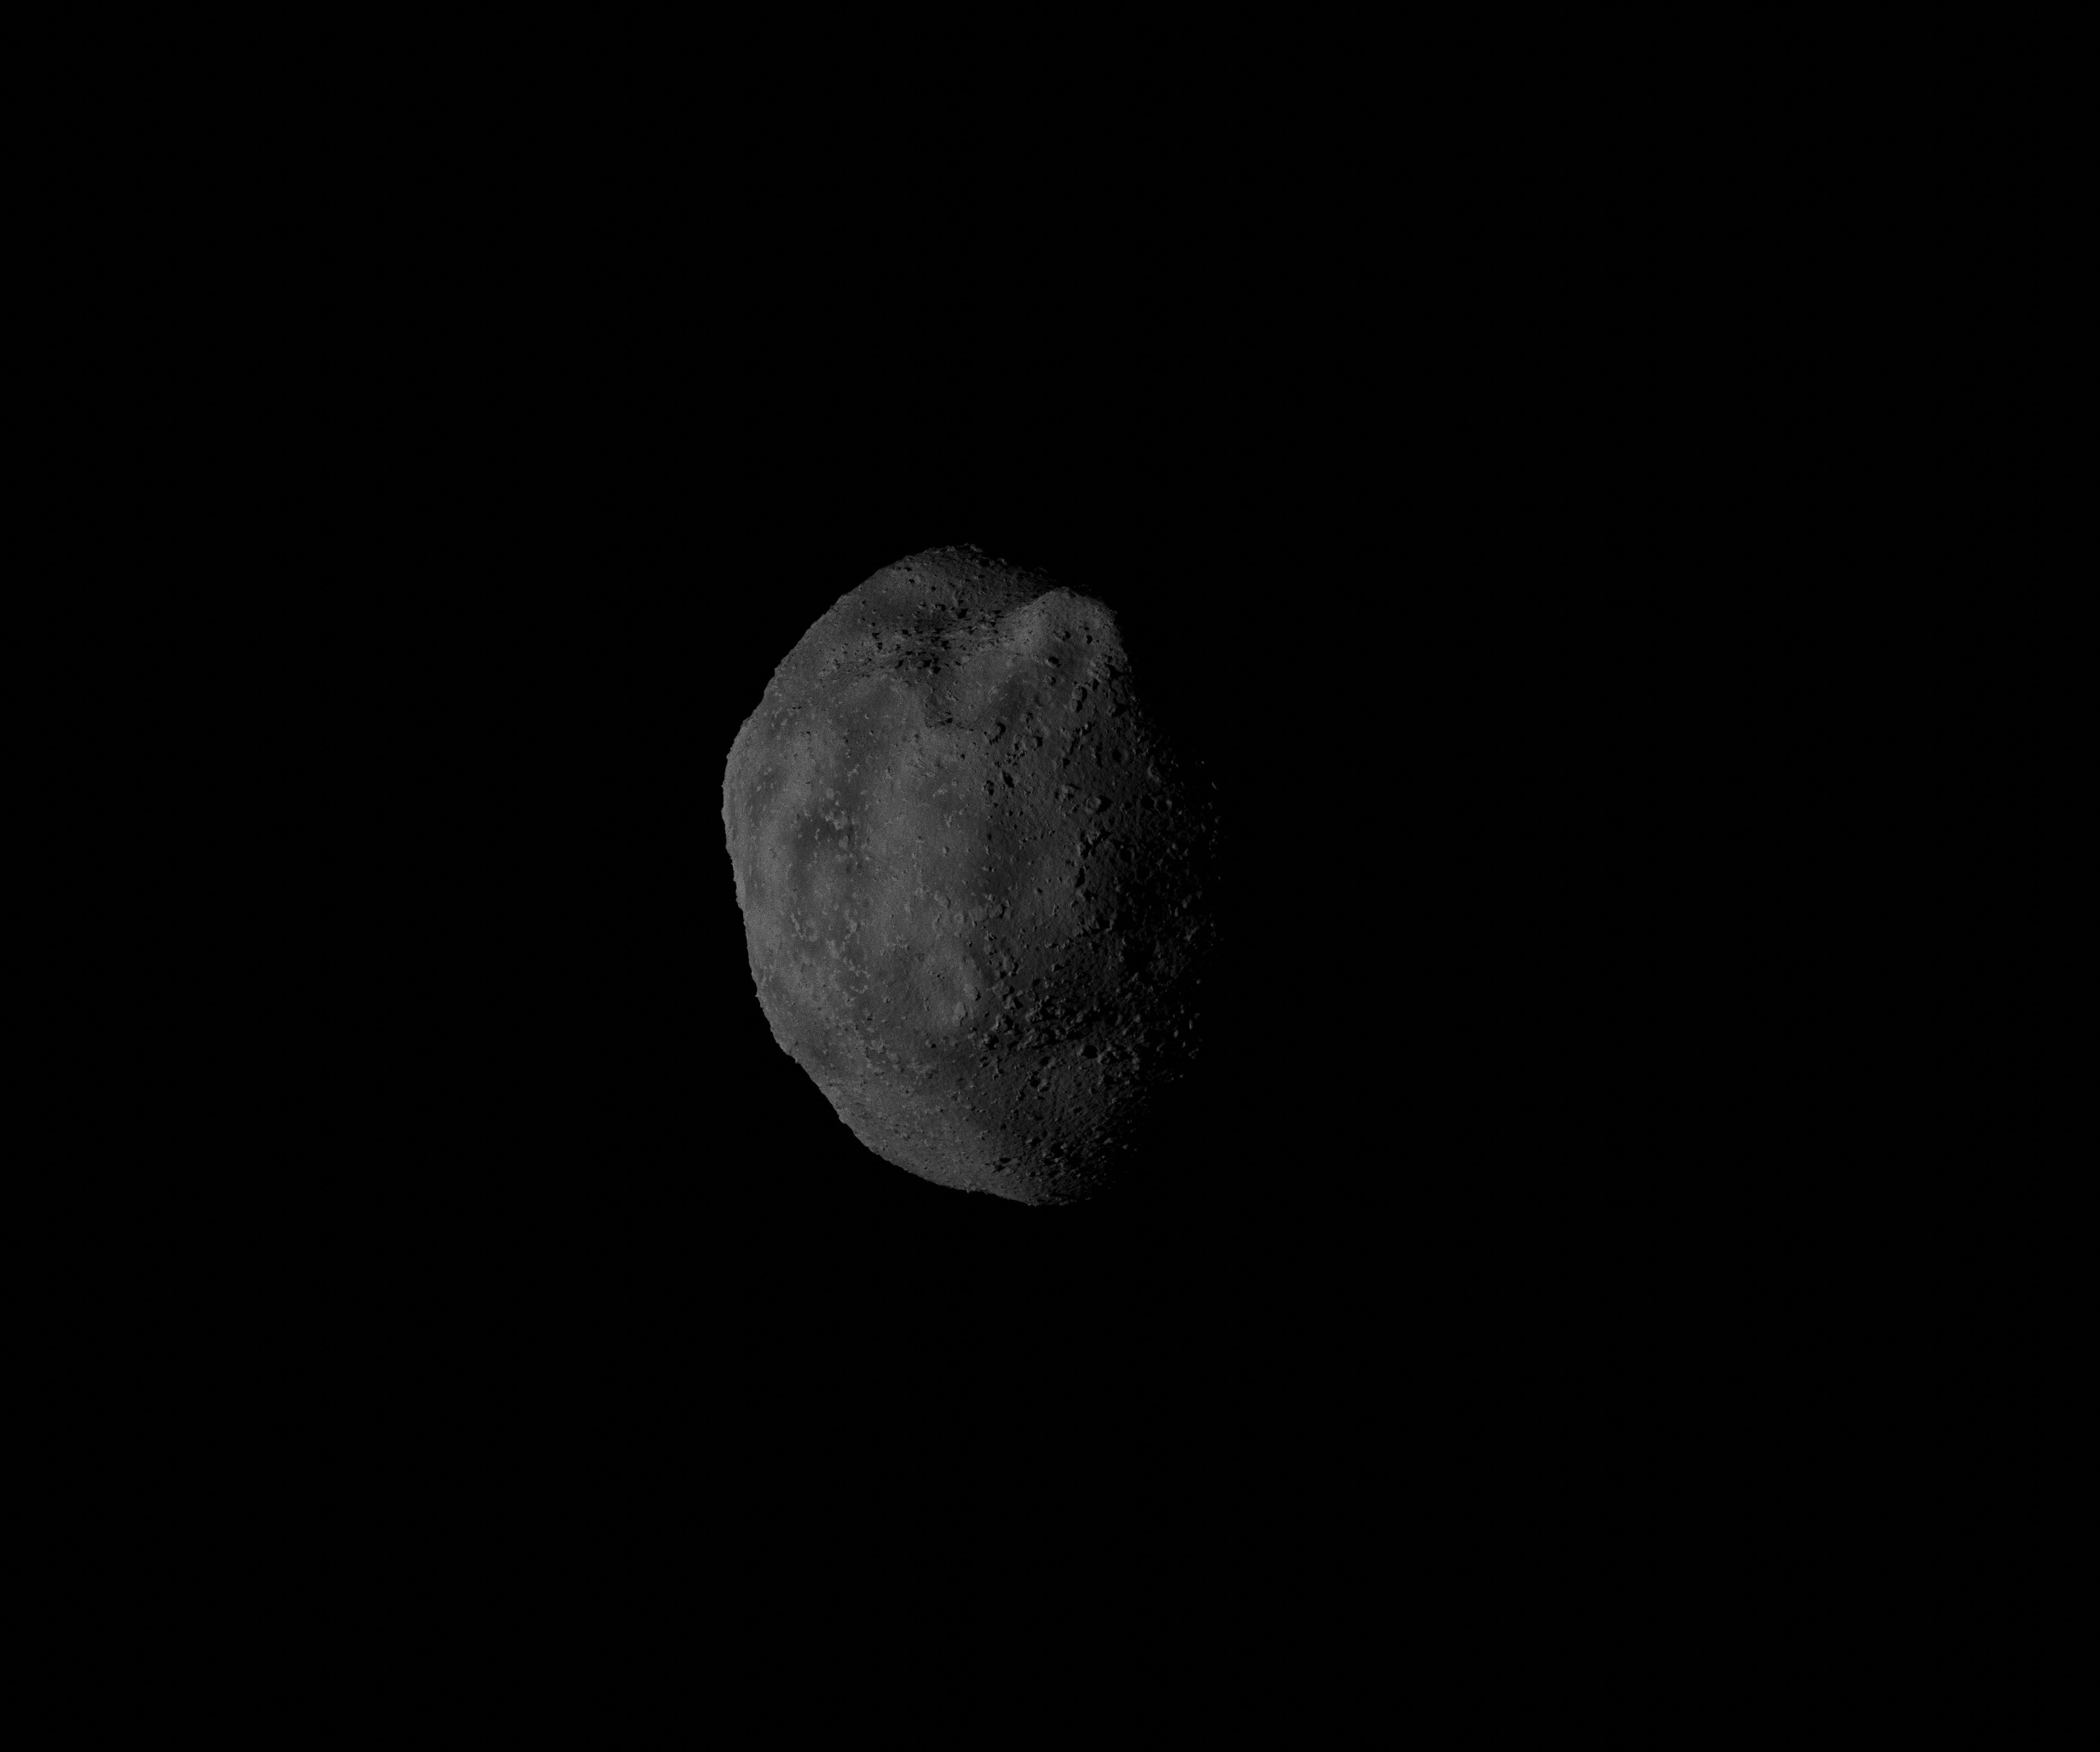
\includegraphics[width=\textwidth]{doc/thesis/0_figures/rendering_lighting/SssbOnly_2017-08-15T115858-281000.jpg}
                \caption{Image 1 before calibration.}
                \label{fig:composition_before_1}
        \end{subfigure}
        \begin{subfigure}[b]{0.48\textwidth}
            \centering
                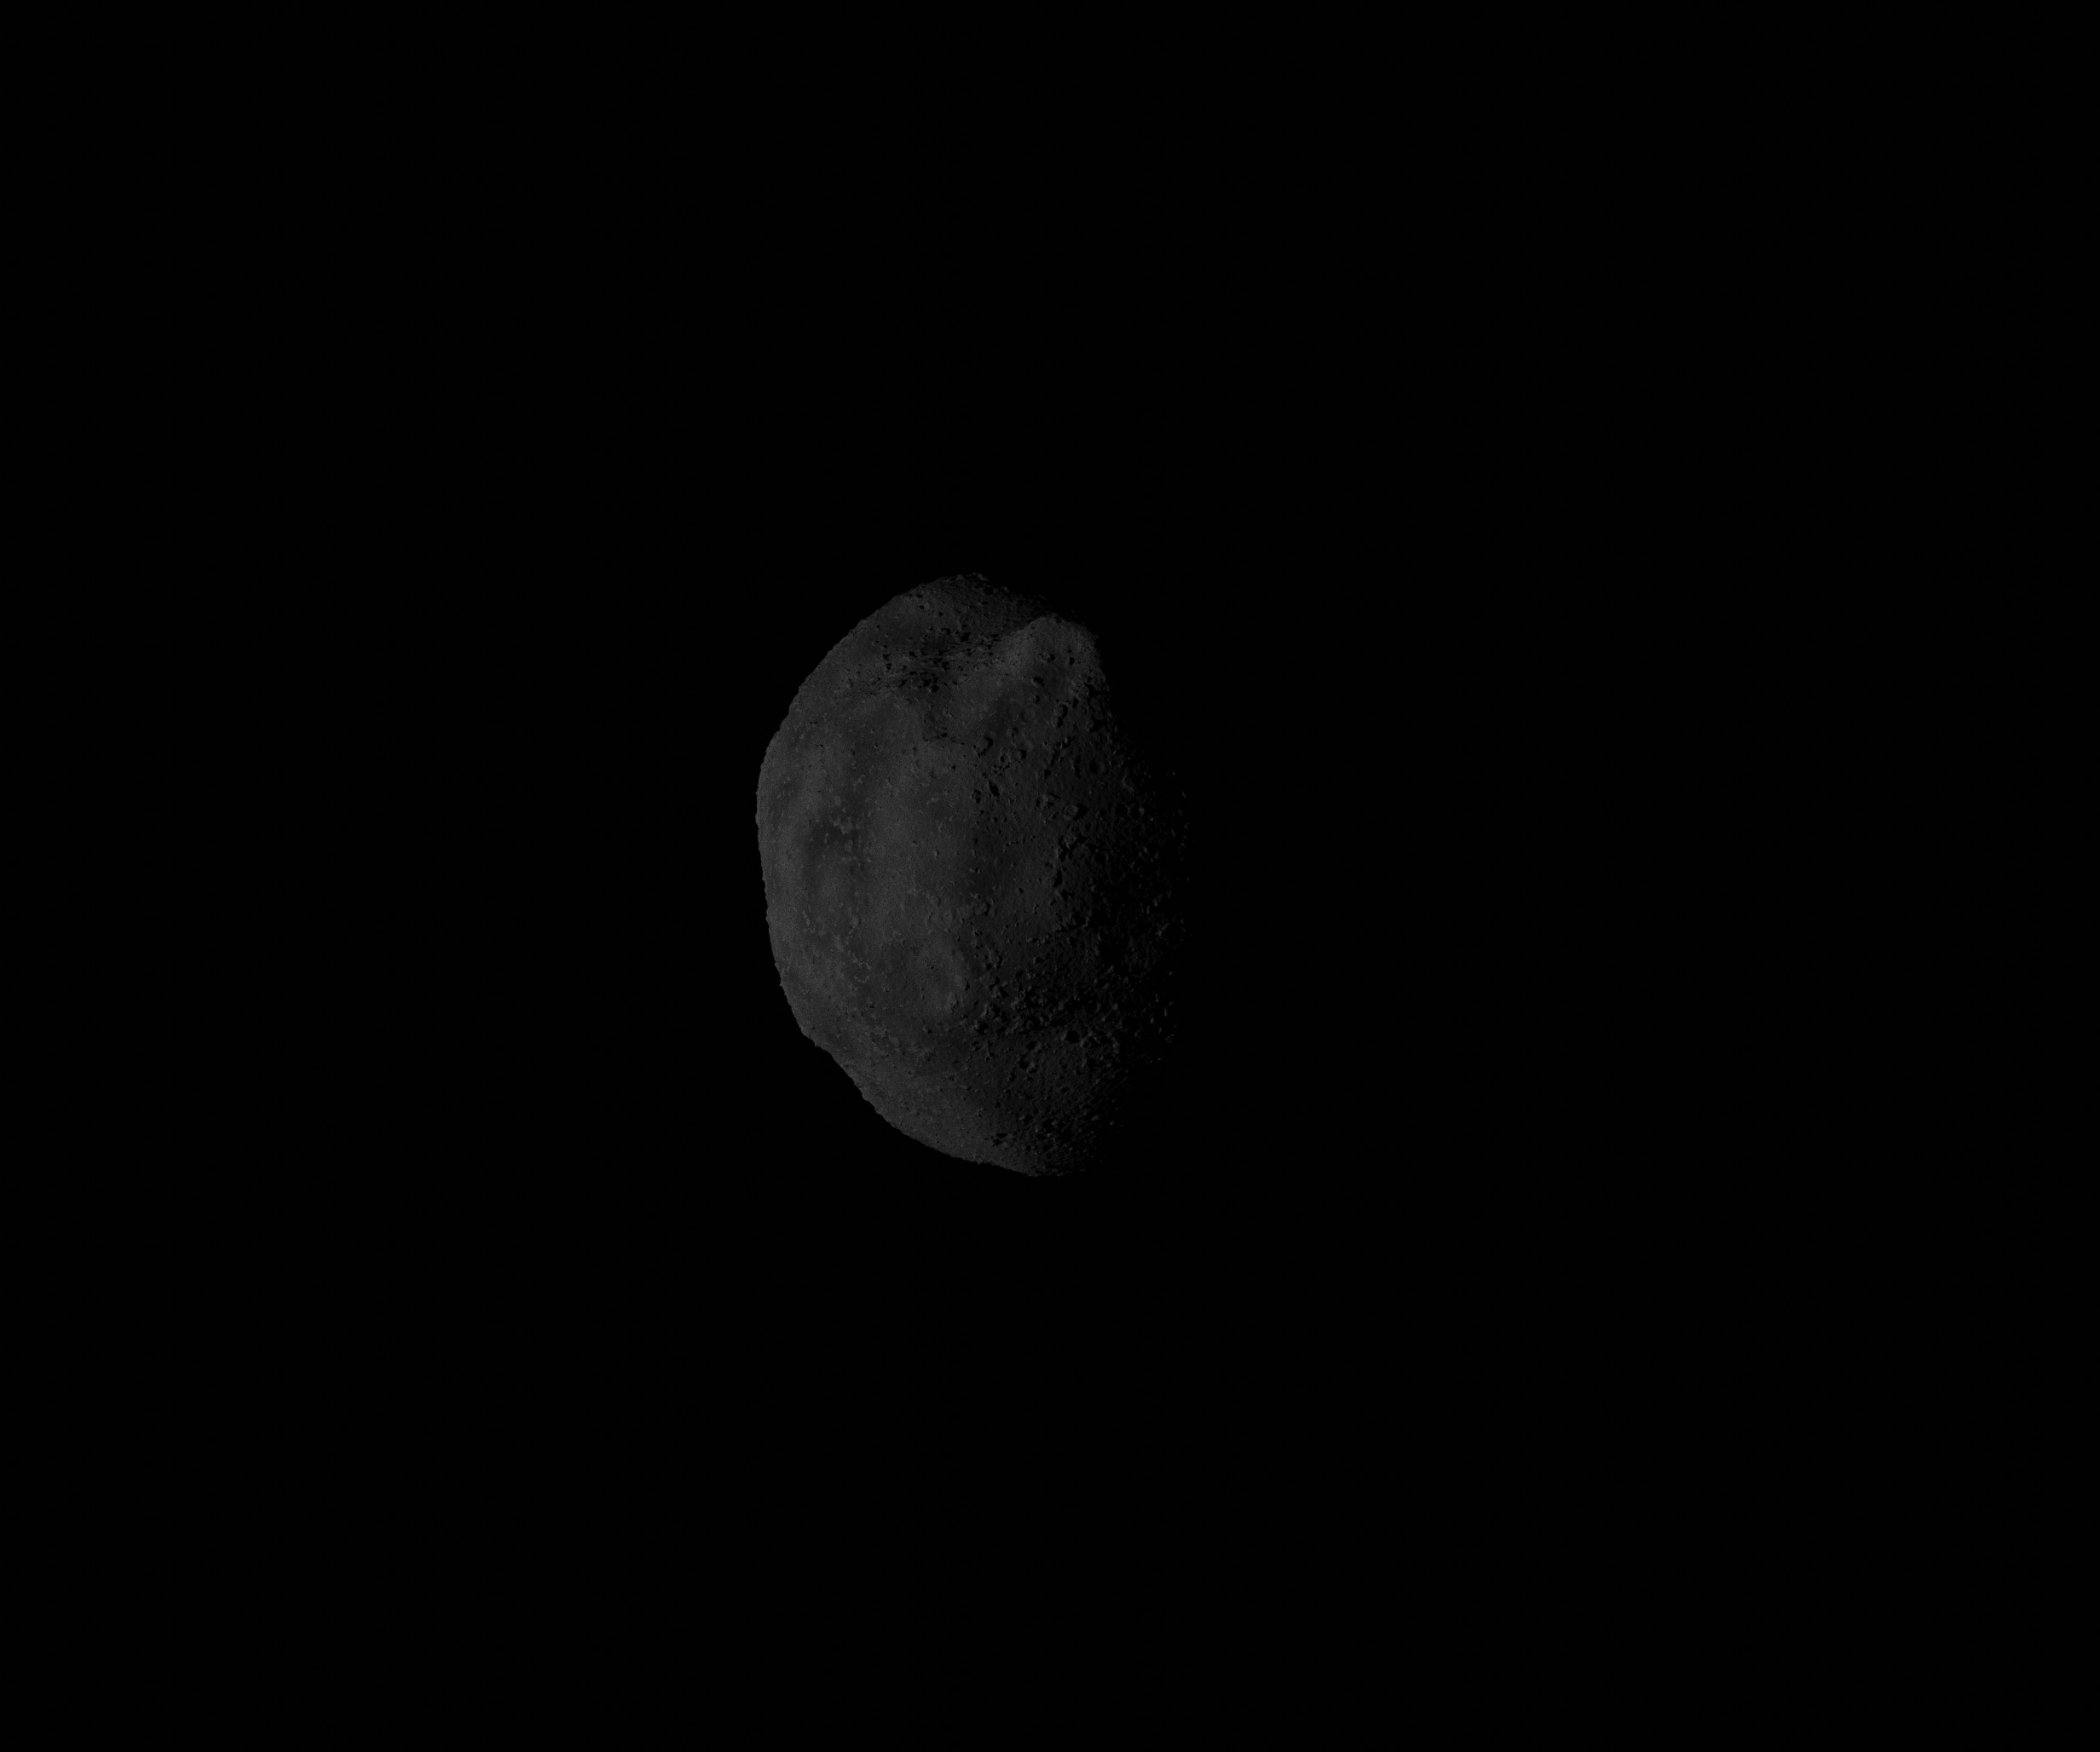
\includegraphics[width=\textwidth]{doc/thesis/0_figures/rendering_lighting/SssbOnly_2017-08-15T115859-288000.jpg}
                \caption{Image 2 before calibration.}
                \label{fig:composition_before_2}
        \end{subfigure}
        \\
        \begin{subfigure}[b]{0.48\textwidth}
            \centering
                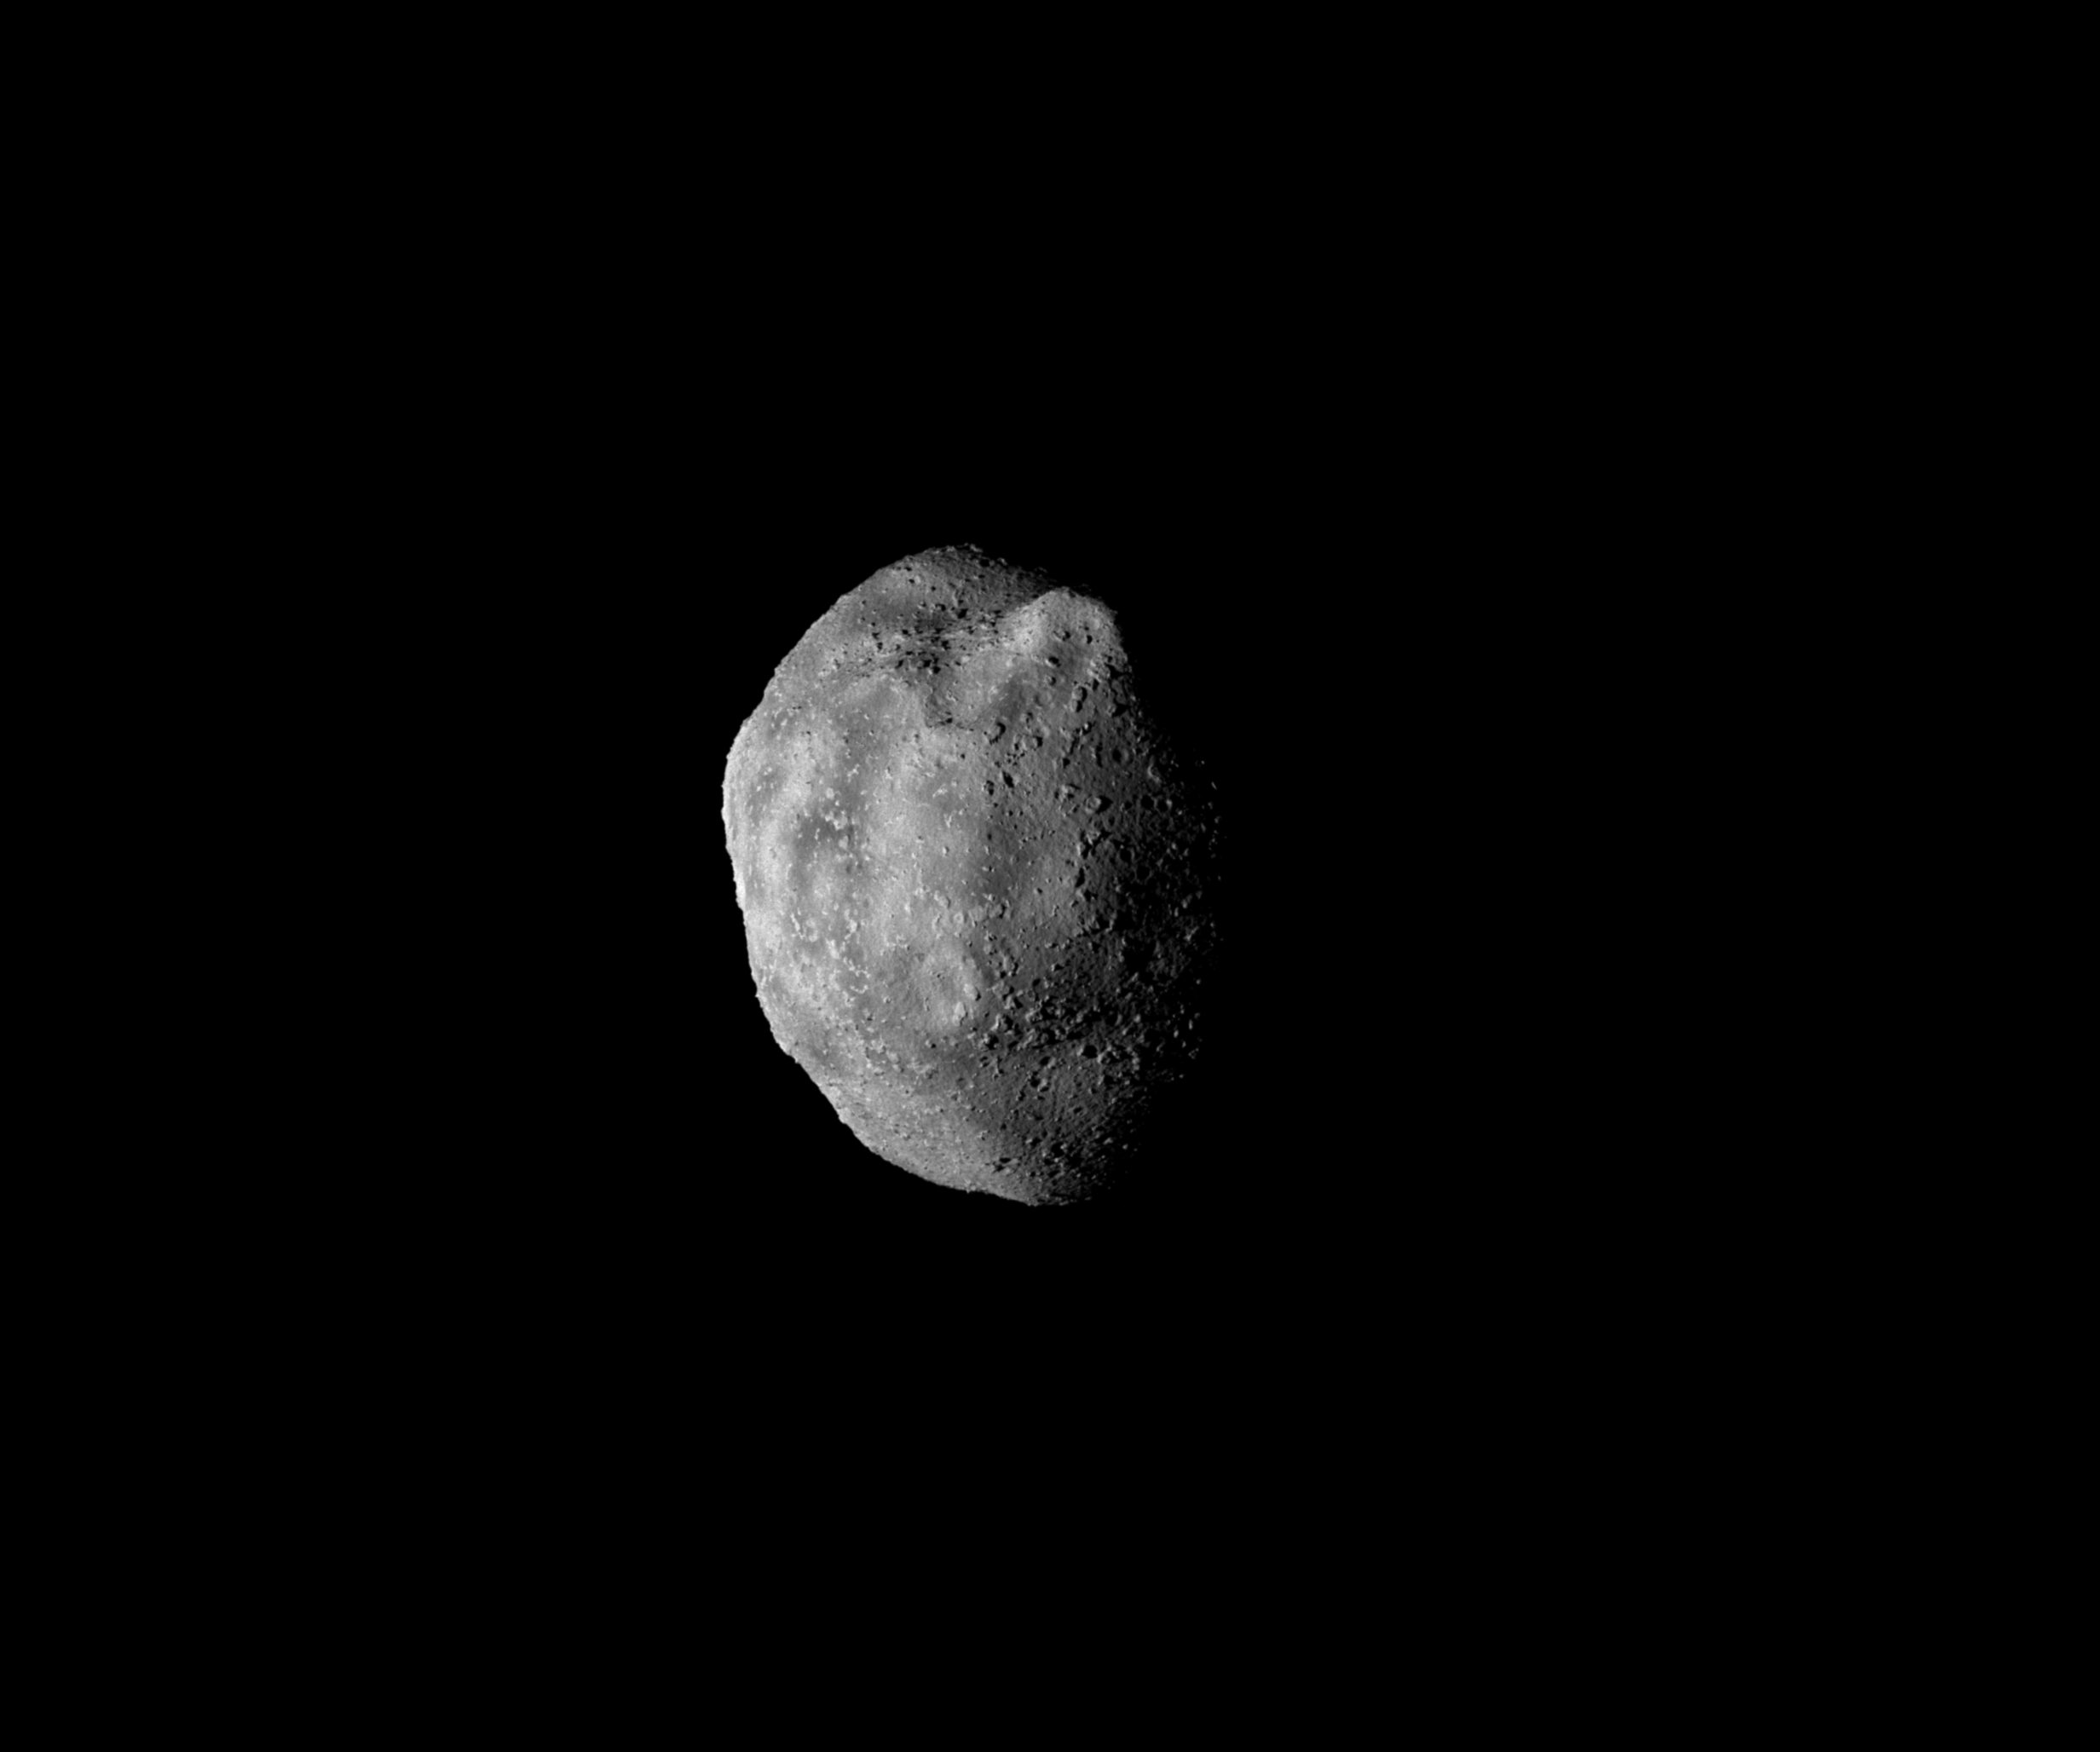
\includegraphics[width=\textwidth]{doc/thesis/0_figures/rendering_lighting/Inst_2017-08-15T115858-281000.png}
                \caption{Image 1 after calibration.}
                \label{fig:composition_after_1}
        \end{subfigure}
        \begin{subfigure}[b]{0.48\textwidth}
            \centering
                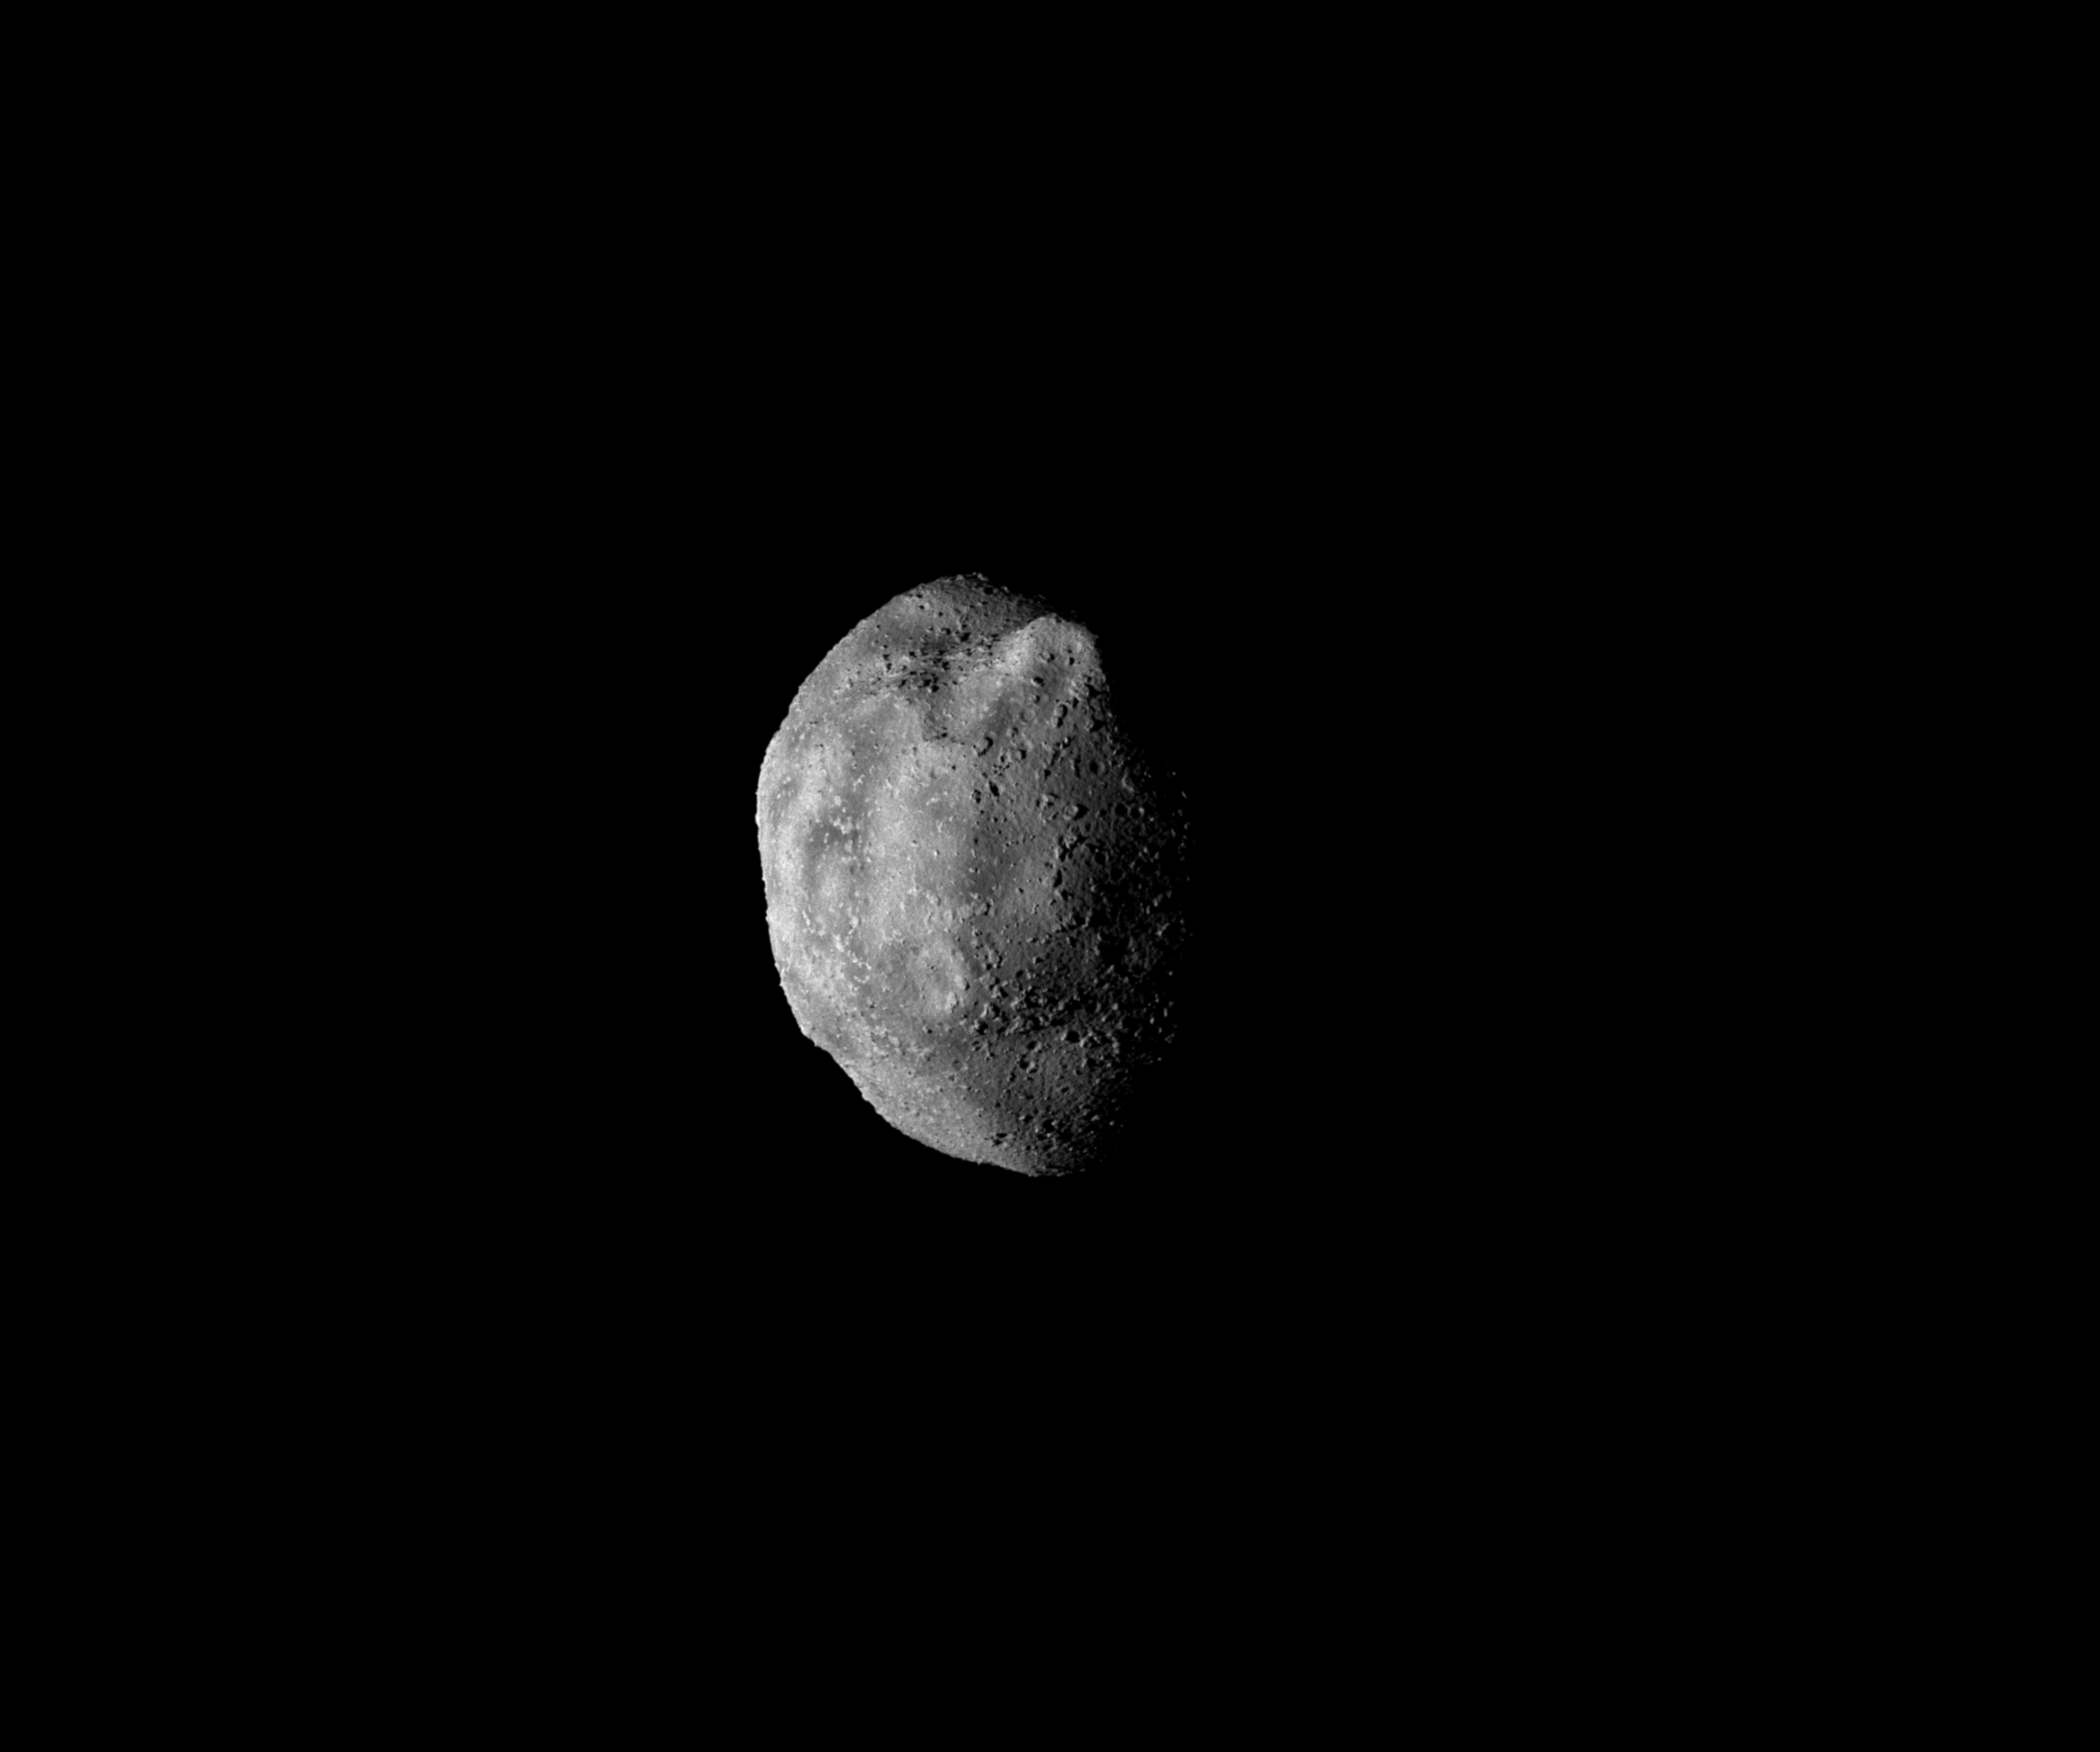
\includegraphics[width=\textwidth]{doc/thesis/0_figures/rendering_lighting/Inst_2017-08-15T115859-288000.png}
                \caption{Image 2 after calibration.}
                \label{fig:composition_after_2}
        \end{subfigure}
        \caption{Two images of a flyby, image 2 is one second after image 1, before and after the composition process. The nucleus is much brighter than background stars thus no stars visible in these images after calibration.}
        \label{fig:composition_before_after}
\end{figure}

% As Figures~\ref{fig:composition_after_1} and \ref{fig:composition_after_2} show, the composition properly calibrates the overall brightness of different images. However, there are sometimes darker and brighter patches within images that are not yet calibrated properly. Figure 

% \begin{figure}[htb]
%     \centering
%         \begin{subfigure}[b]{0.32\textwidth}
%             \centering
%             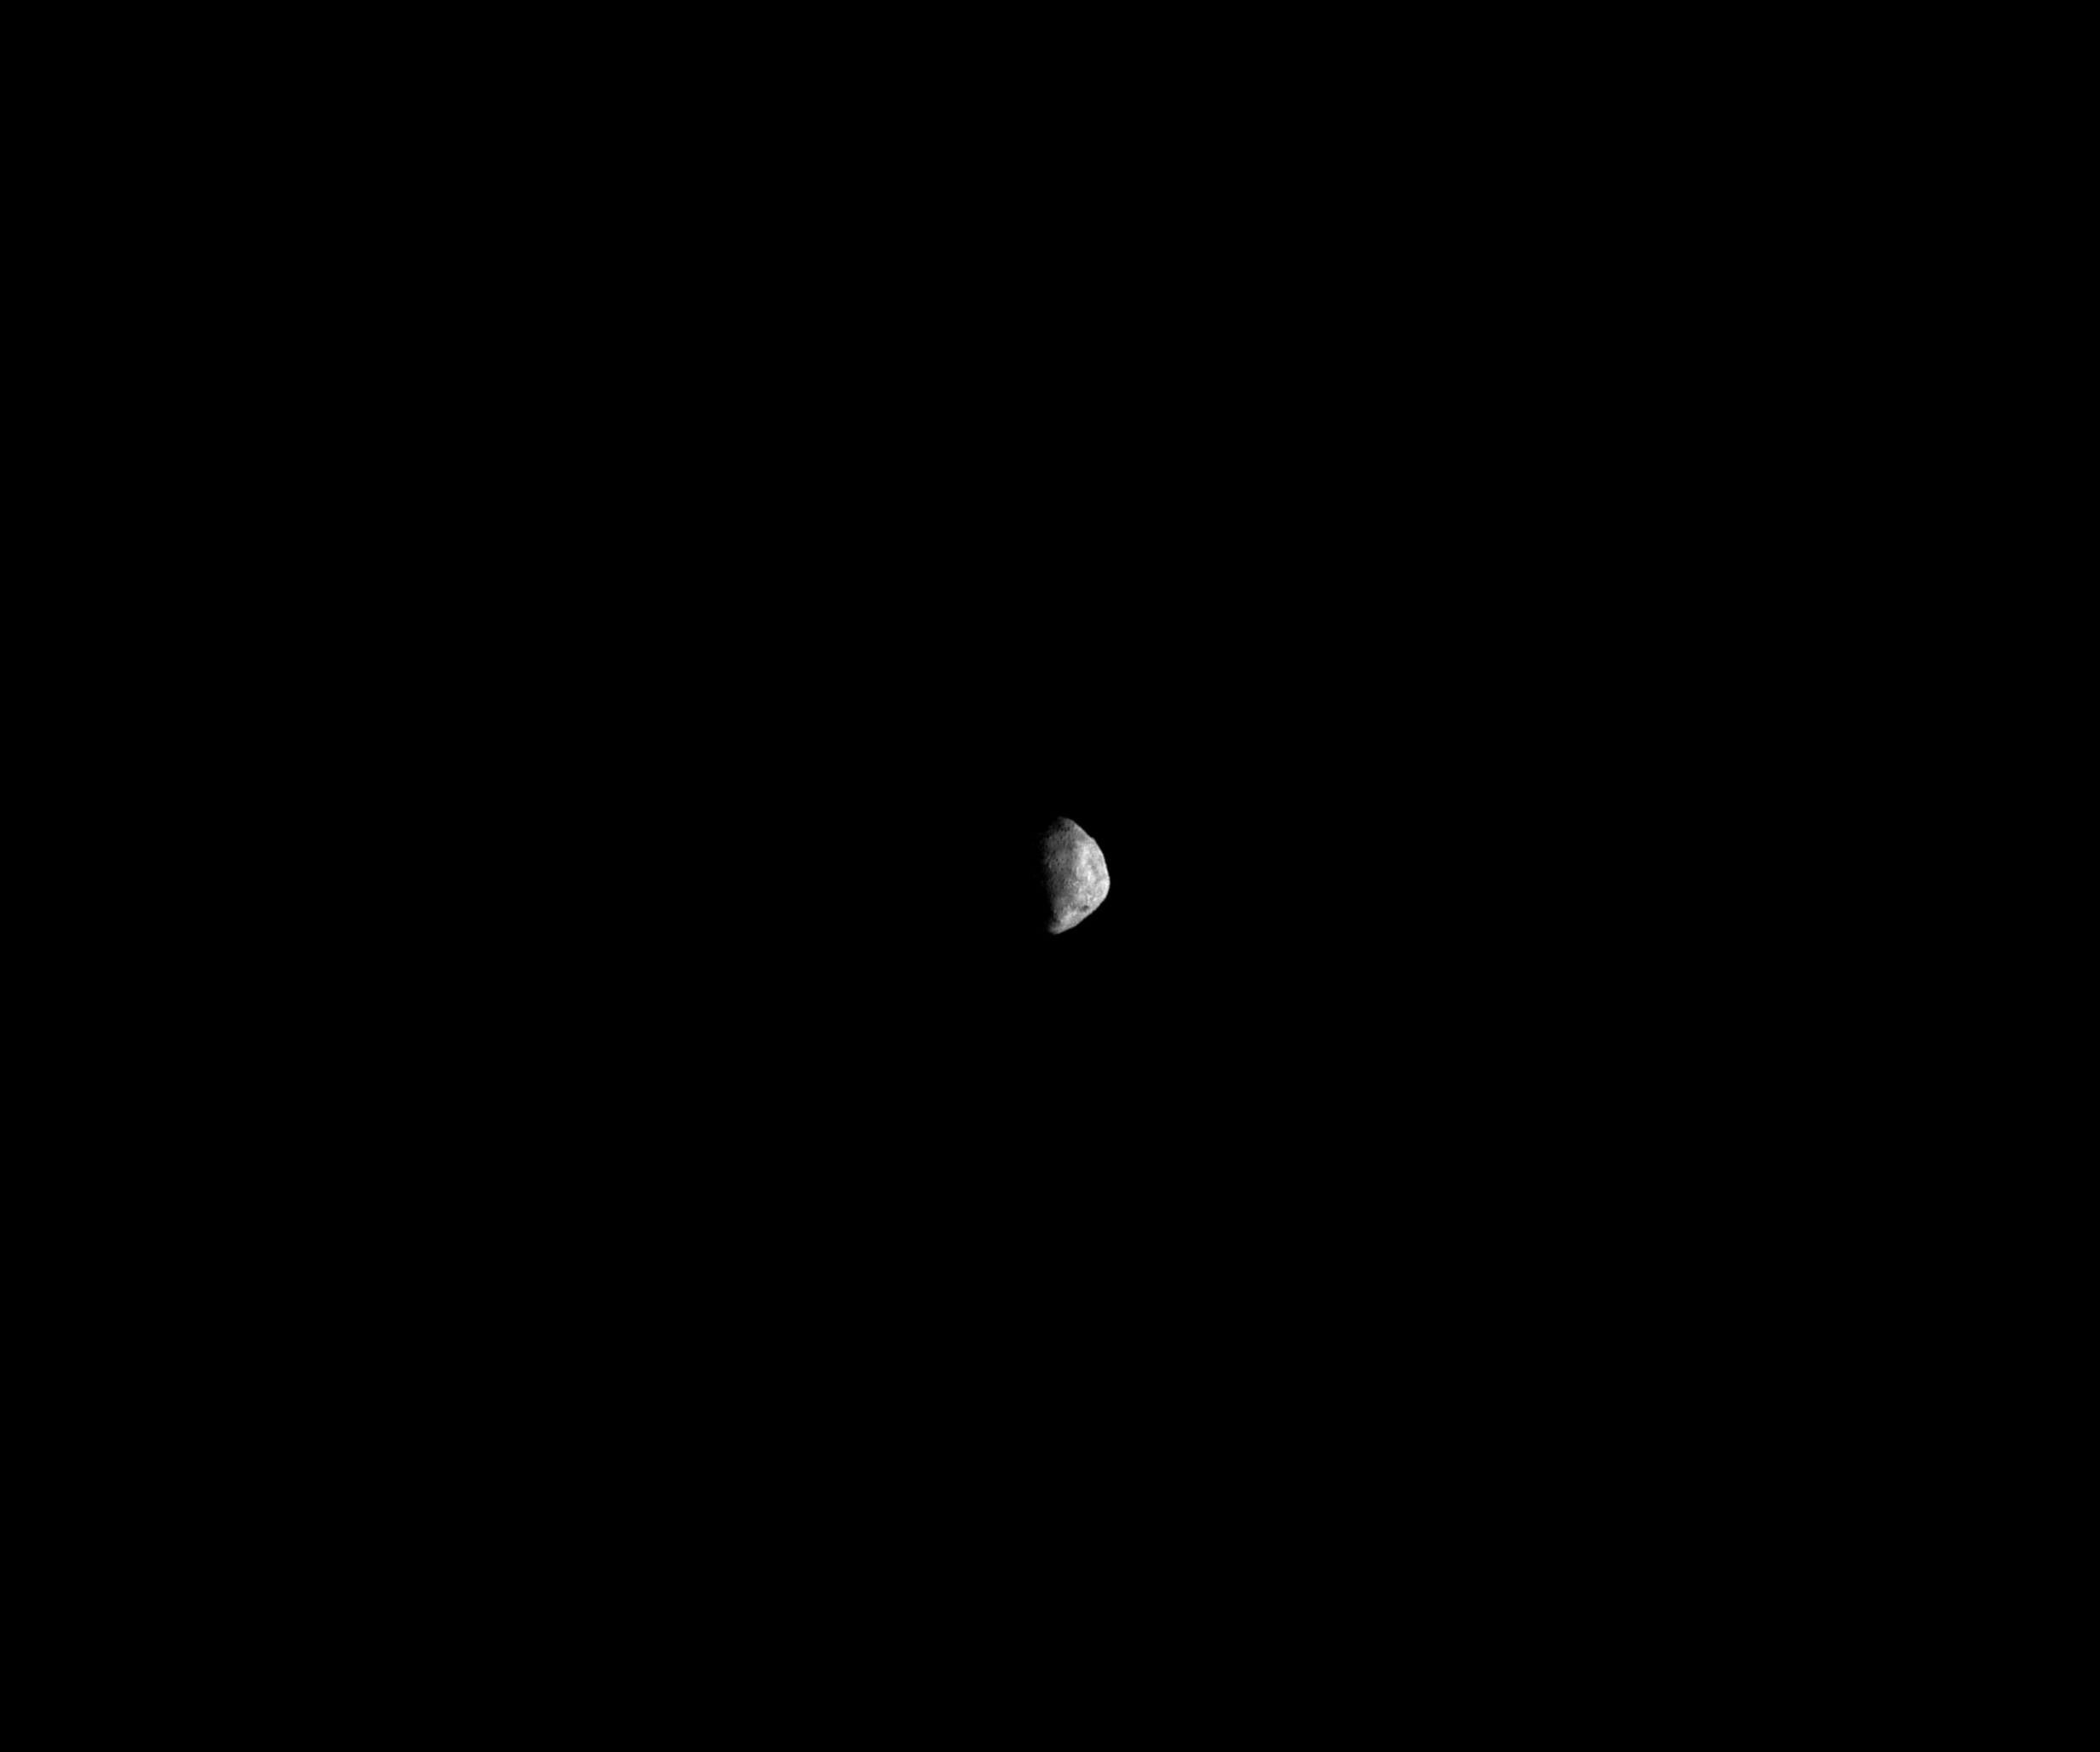
\includegraphics[width=\textwidth]{doc/thesis/0_figures/composition_varying_brightness/Inst_2017-08-15T115803-901000.png}
%             \label{fig:composition_varying_1}
%         \end{subfigure}
%         \begin{subfigure}[b]{0.32\textwidth}
%             \centering
%             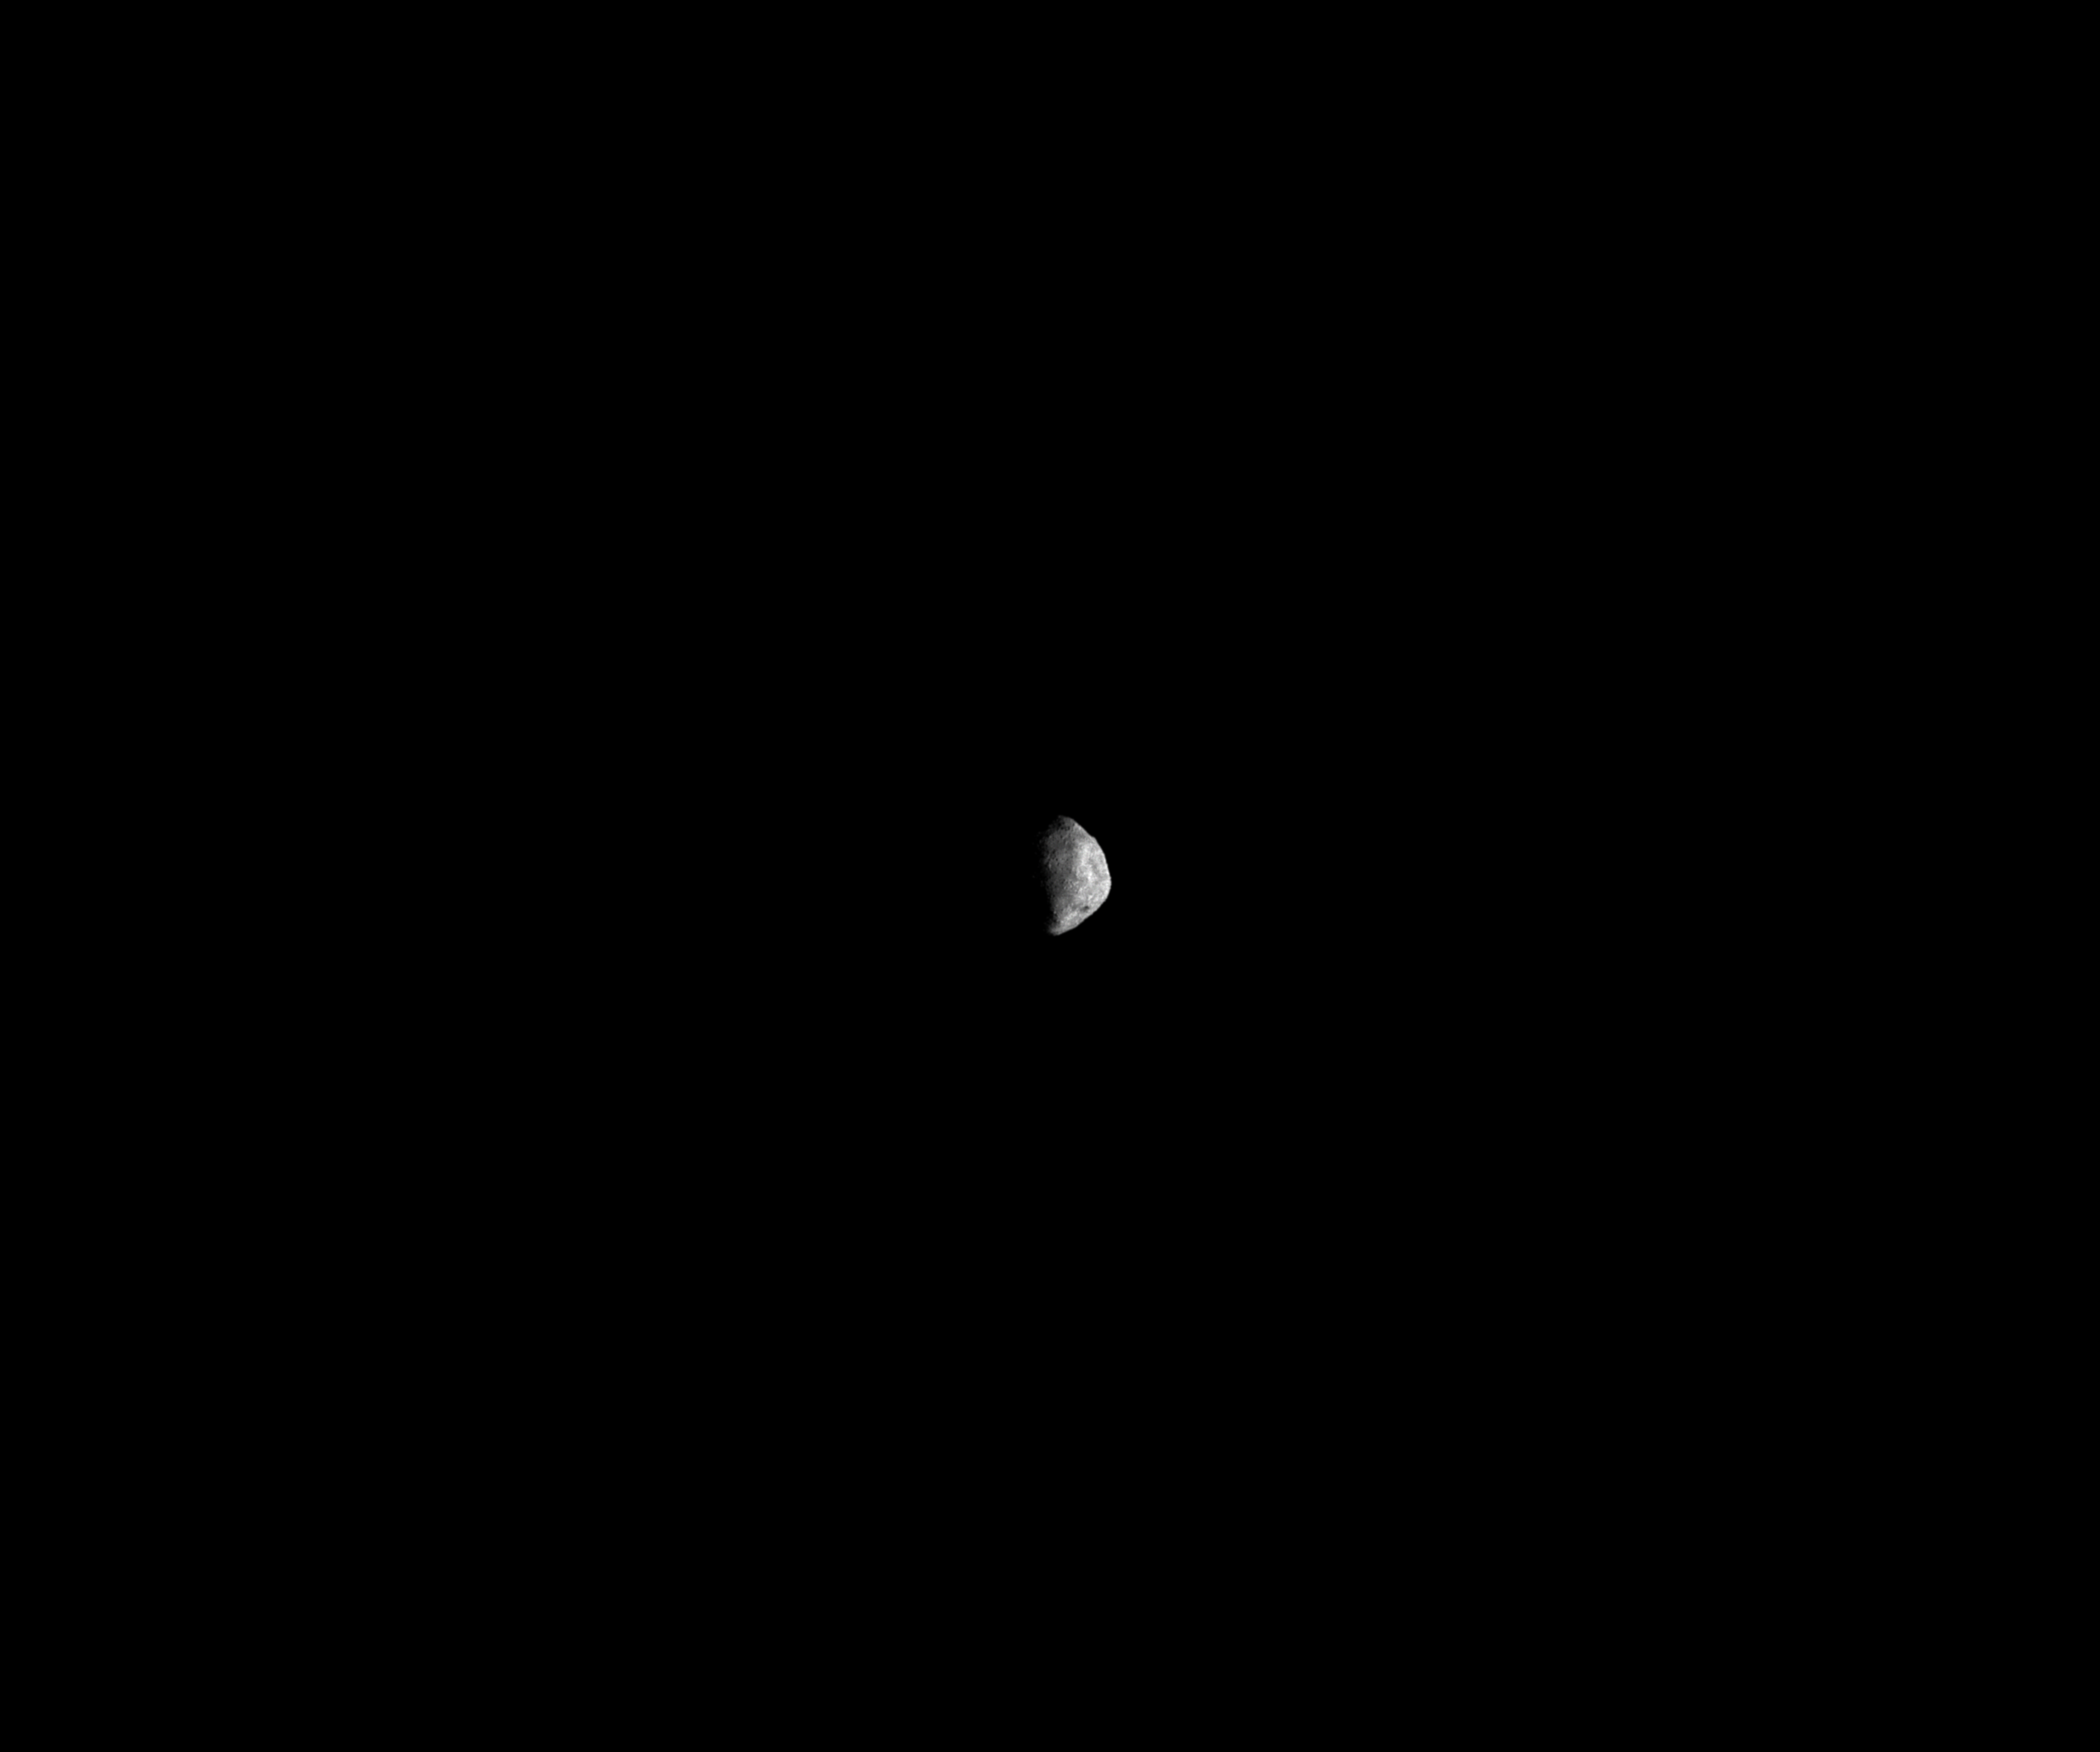
\includegraphics[width=\textwidth]{doc/thesis/0_figures/composition_varying_brightness/Inst_2017-08-15T115804-908000.png}
%             \label{fig:composition_varying_2}
%         \end{subfigure}
%         \begin{subfigure}[b]{0.32\textwidth}
%             \centering
%             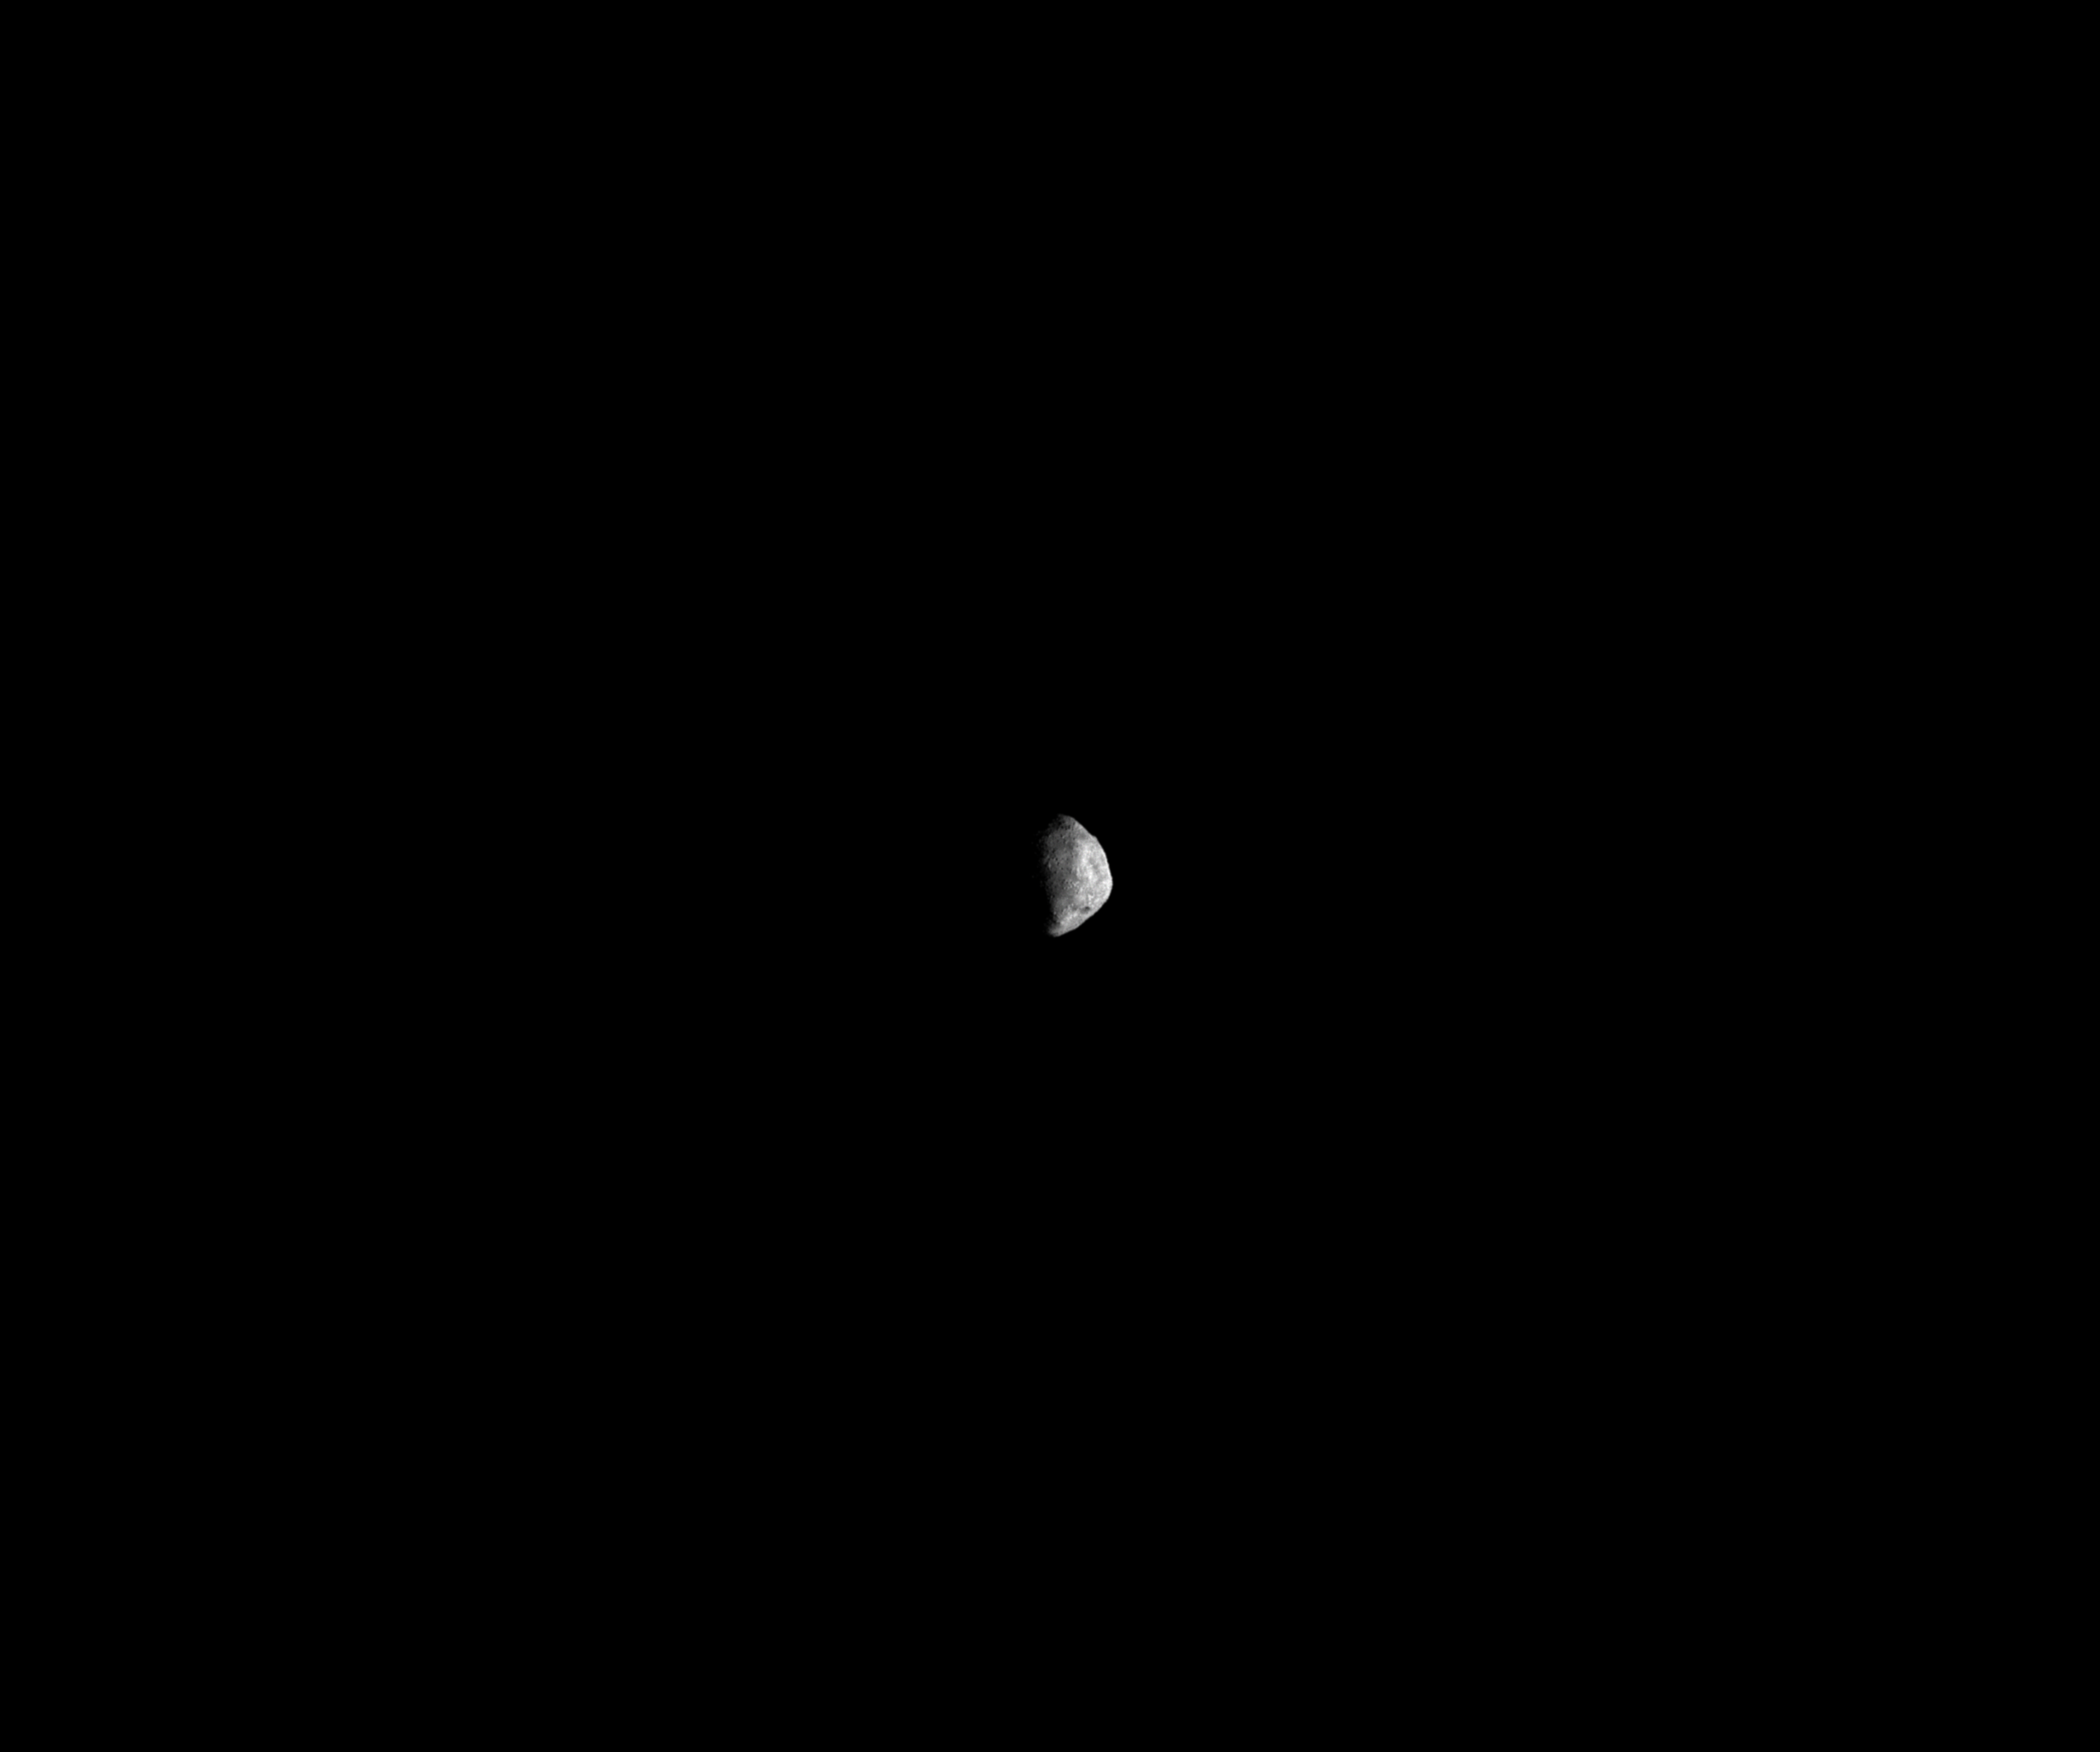
\includegraphics[width=\textwidth]{doc/thesis/0_figures/composition_varying_brightness/Inst_2017-08-15T115805-915000.png}
%             \label{fig:composition_varying_3}
%         \end{subfigure}
%     \caption{Varying brightness of patches on the \gls{sssb} surface.}
%     \label{fig:composition_varying}
% \end{figure}

\subsubsection{Rendering Problems} \label{sec:render_problems}
Rendering a fly-by scenario with a \SI{10}{\kilo\meter} \gls{sssb} created artefacts in the images. Figure~\ref{fig:render_artefacts} shows renders from flybys with different closest distances from the nucleus. All three images are the raw output from rendering, before composition. The images show a stripe, a darker patch across the \gls{sssb} with sharp brightness transitions. Moreover, the stripe is at the same location across the \gls{sssb} in all three images. This type of artefact does not appear for other \gls{sssb} sizes. The most likely explanation are errors while scaling the nucleus from the original \SI{1}{\kilo\meter} to the \SI{10}{\kilo\meter} model.
\begin{figure}[htb]
    \centering
        \begin{subfigure}[b]{0.32\textwidth}
            \centering
            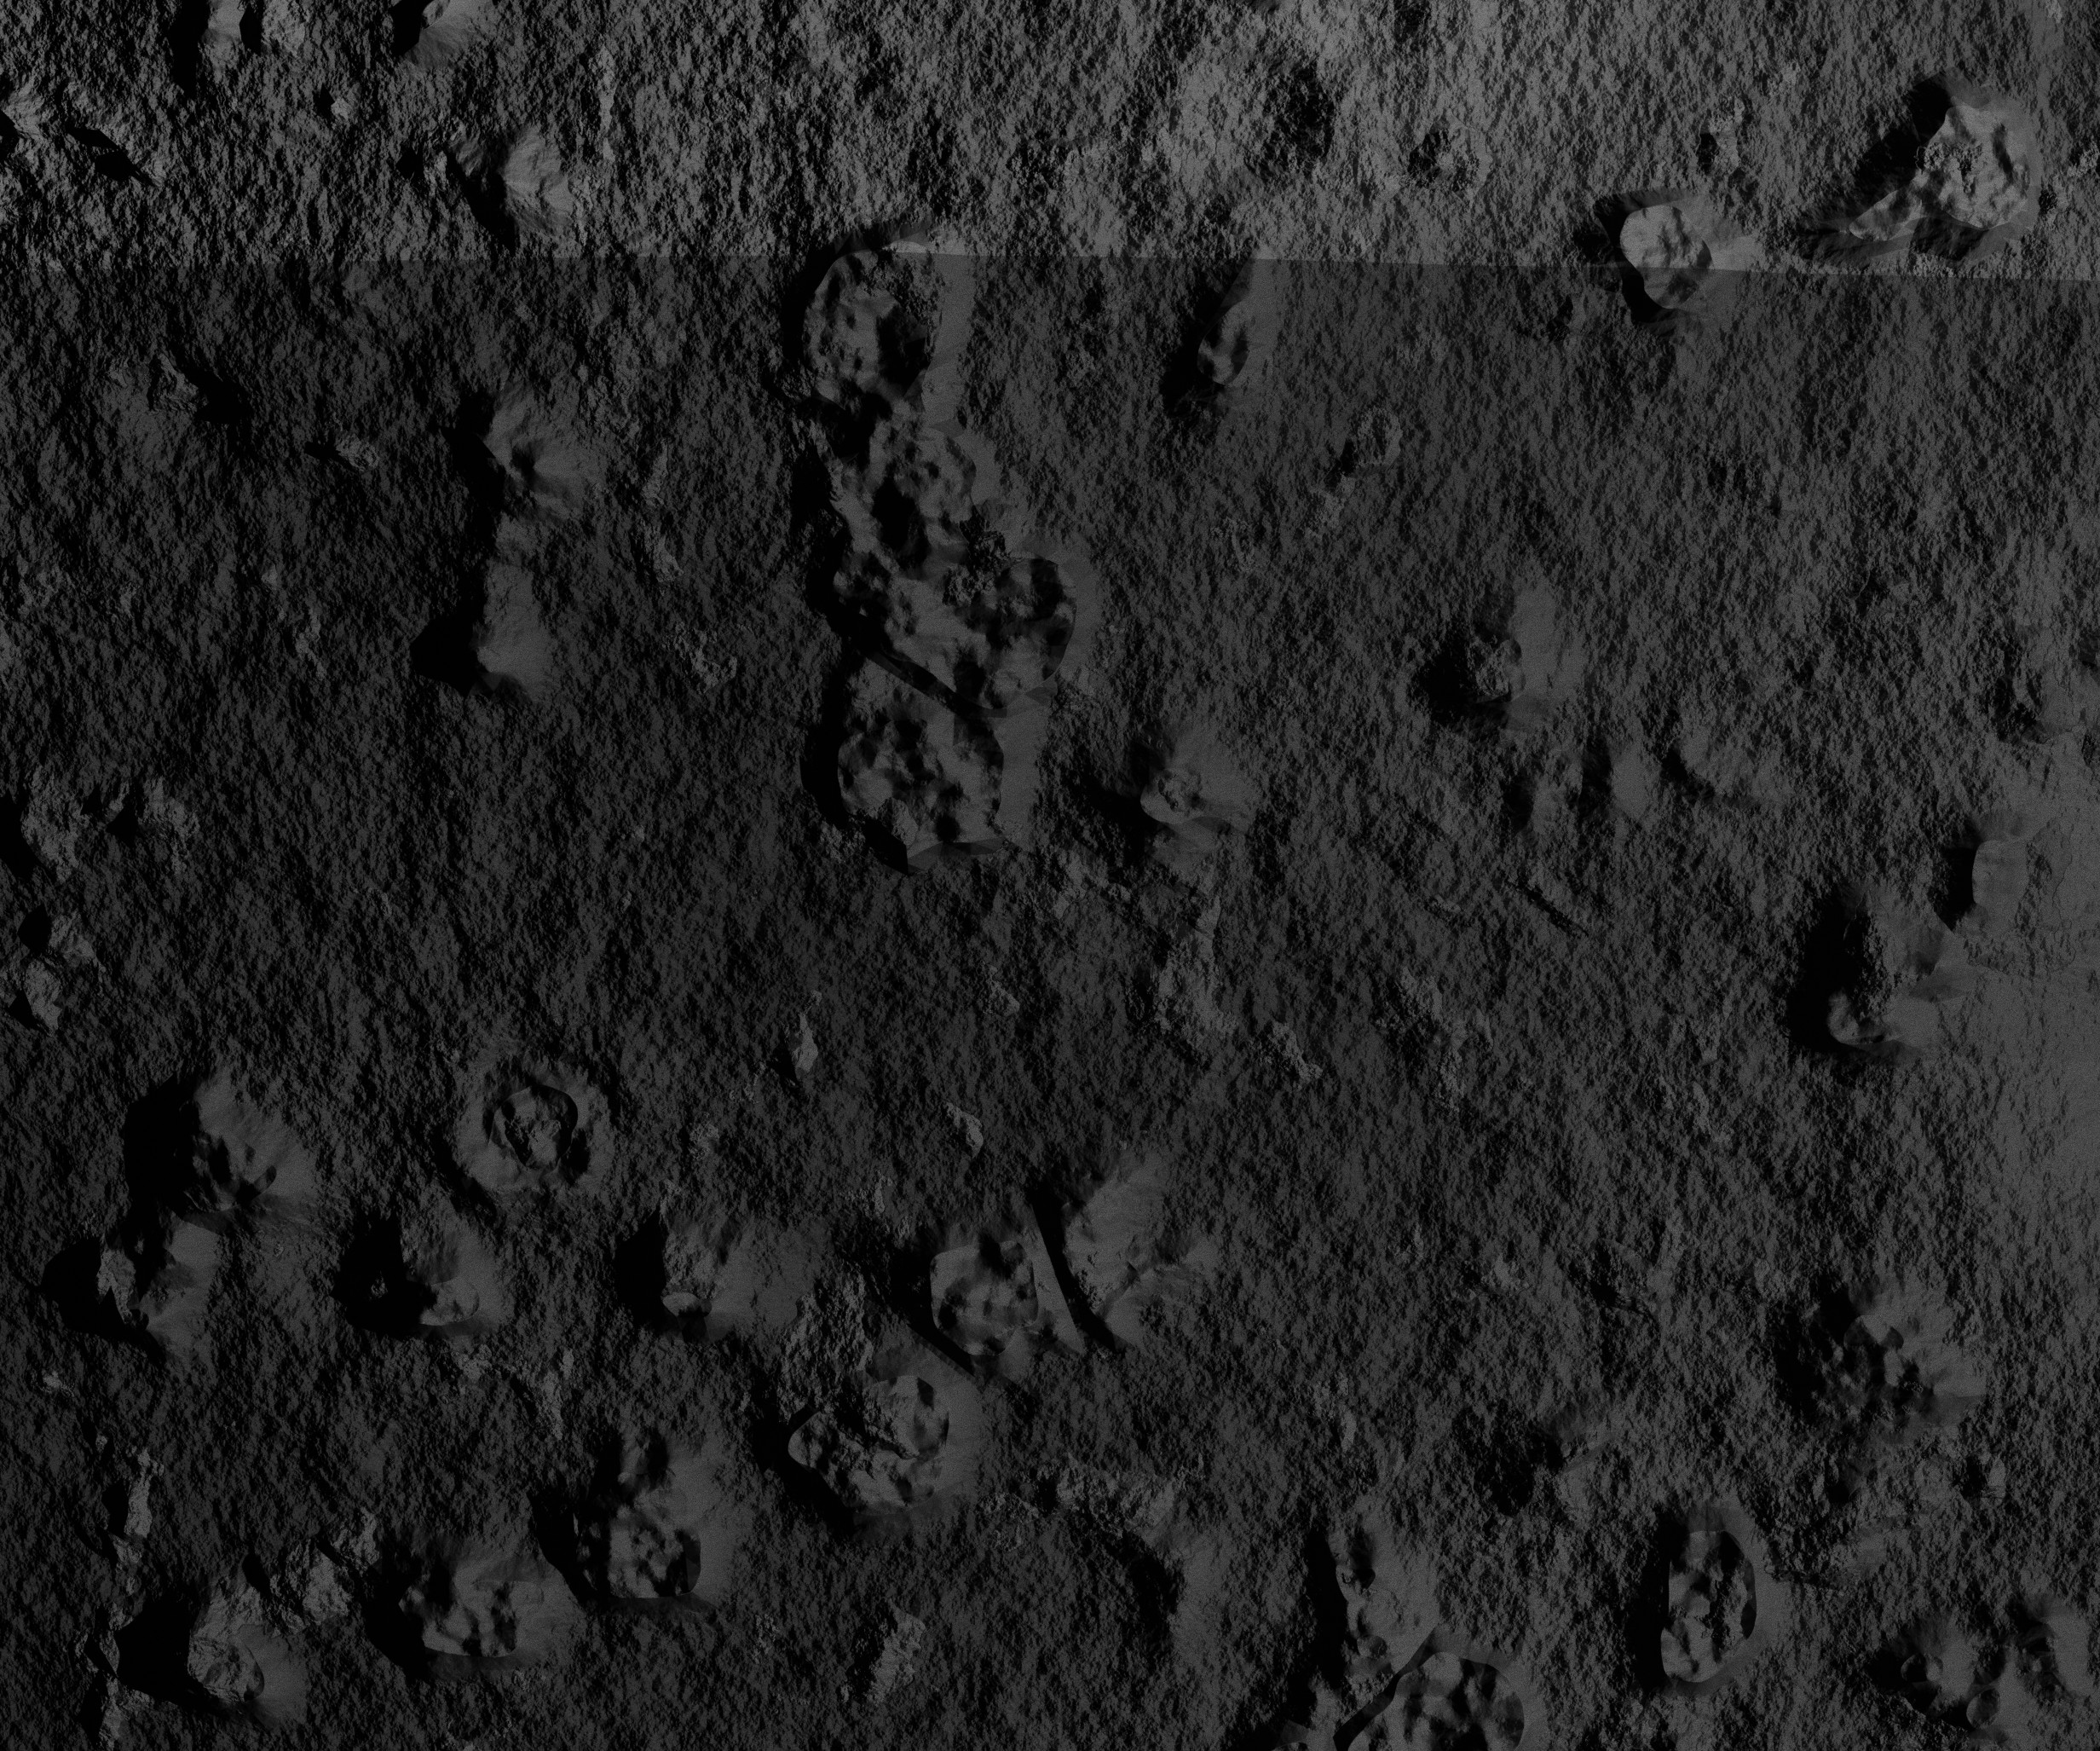
\includegraphics[width=\textwidth]{doc/thesis/0_figures/rendering_artefacts/50_10_SssbOnly_2017-08-15T115845-190000.jpg}
            \caption{\SI{50}{\kilo\meter}.}
            \label{fig:render_artefacts_50}
        \end{subfigure}
        \begin{subfigure}[b]{0.32\textwidth}
            \centering
            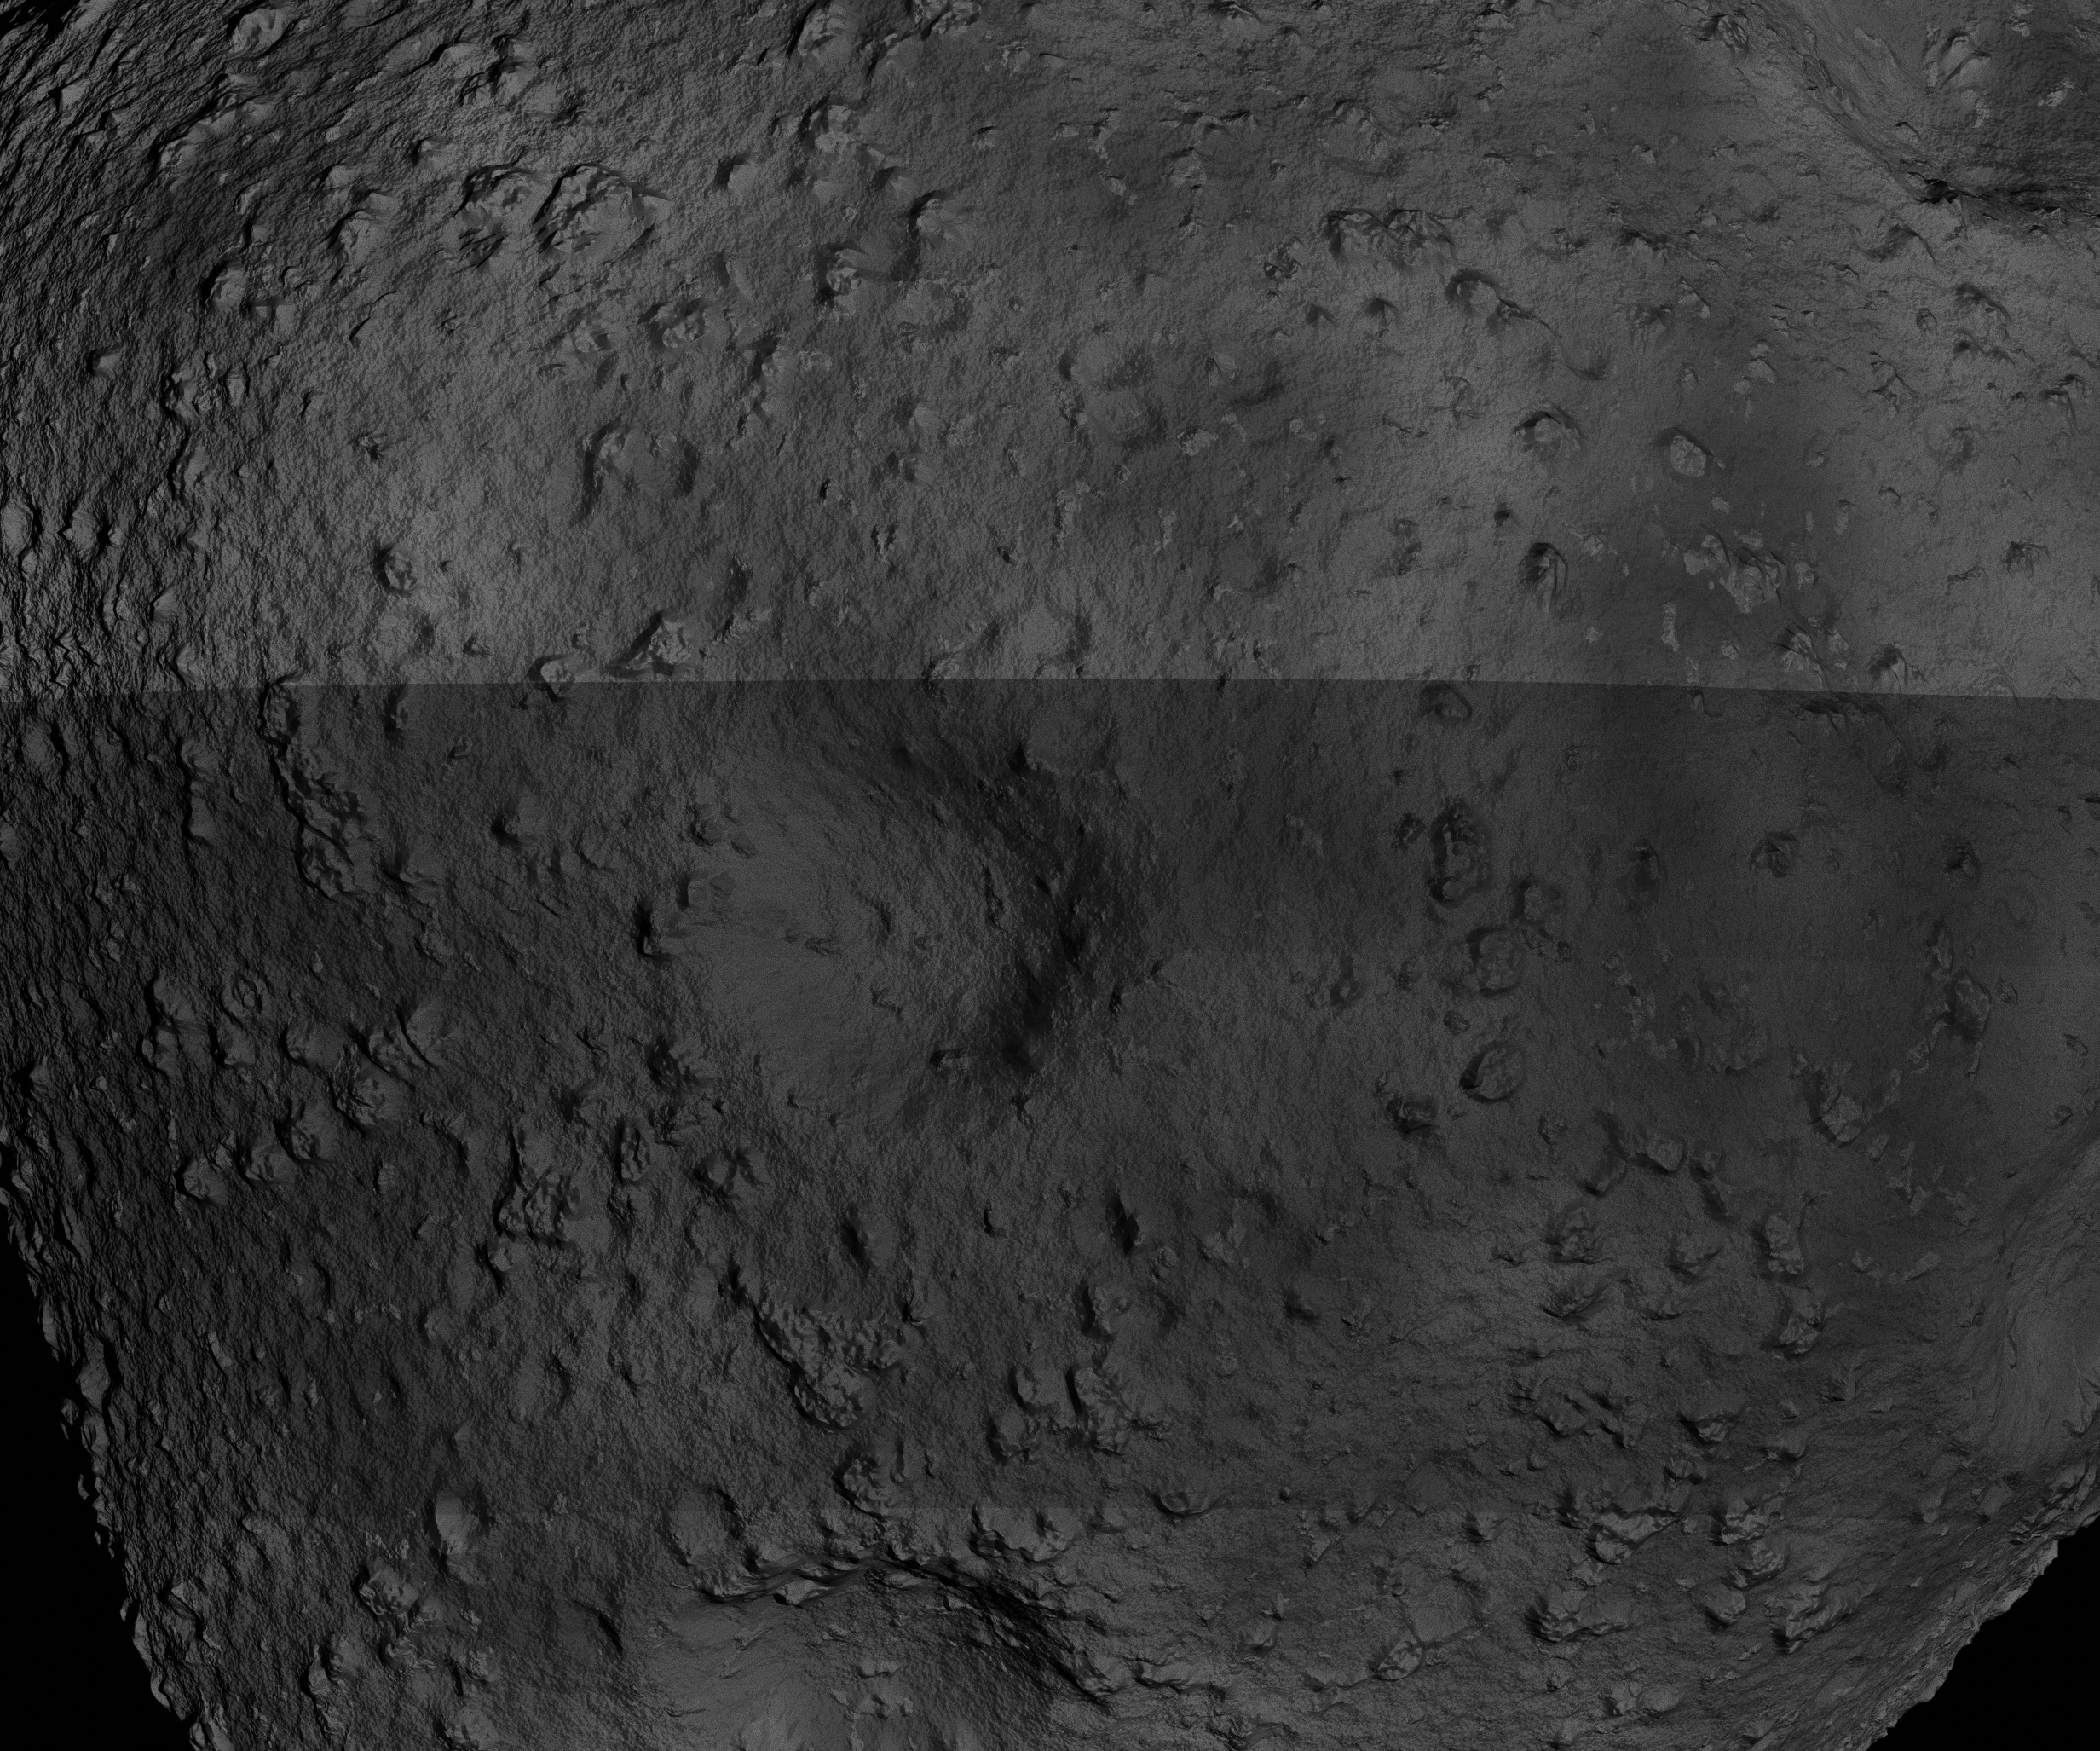
\includegraphics[width=\textwidth]{doc/thesis/0_figures/rendering_artefacts/200_10_SssbOnly_2017-08-15T115845-190000.jpg}
            \caption{\SI{200}{\kilo\meter}.}
            \label{fig:render_artefacts_200}
        \end{subfigure}
        \begin{subfigure}[b]{0.32\textwidth}
            \centering
            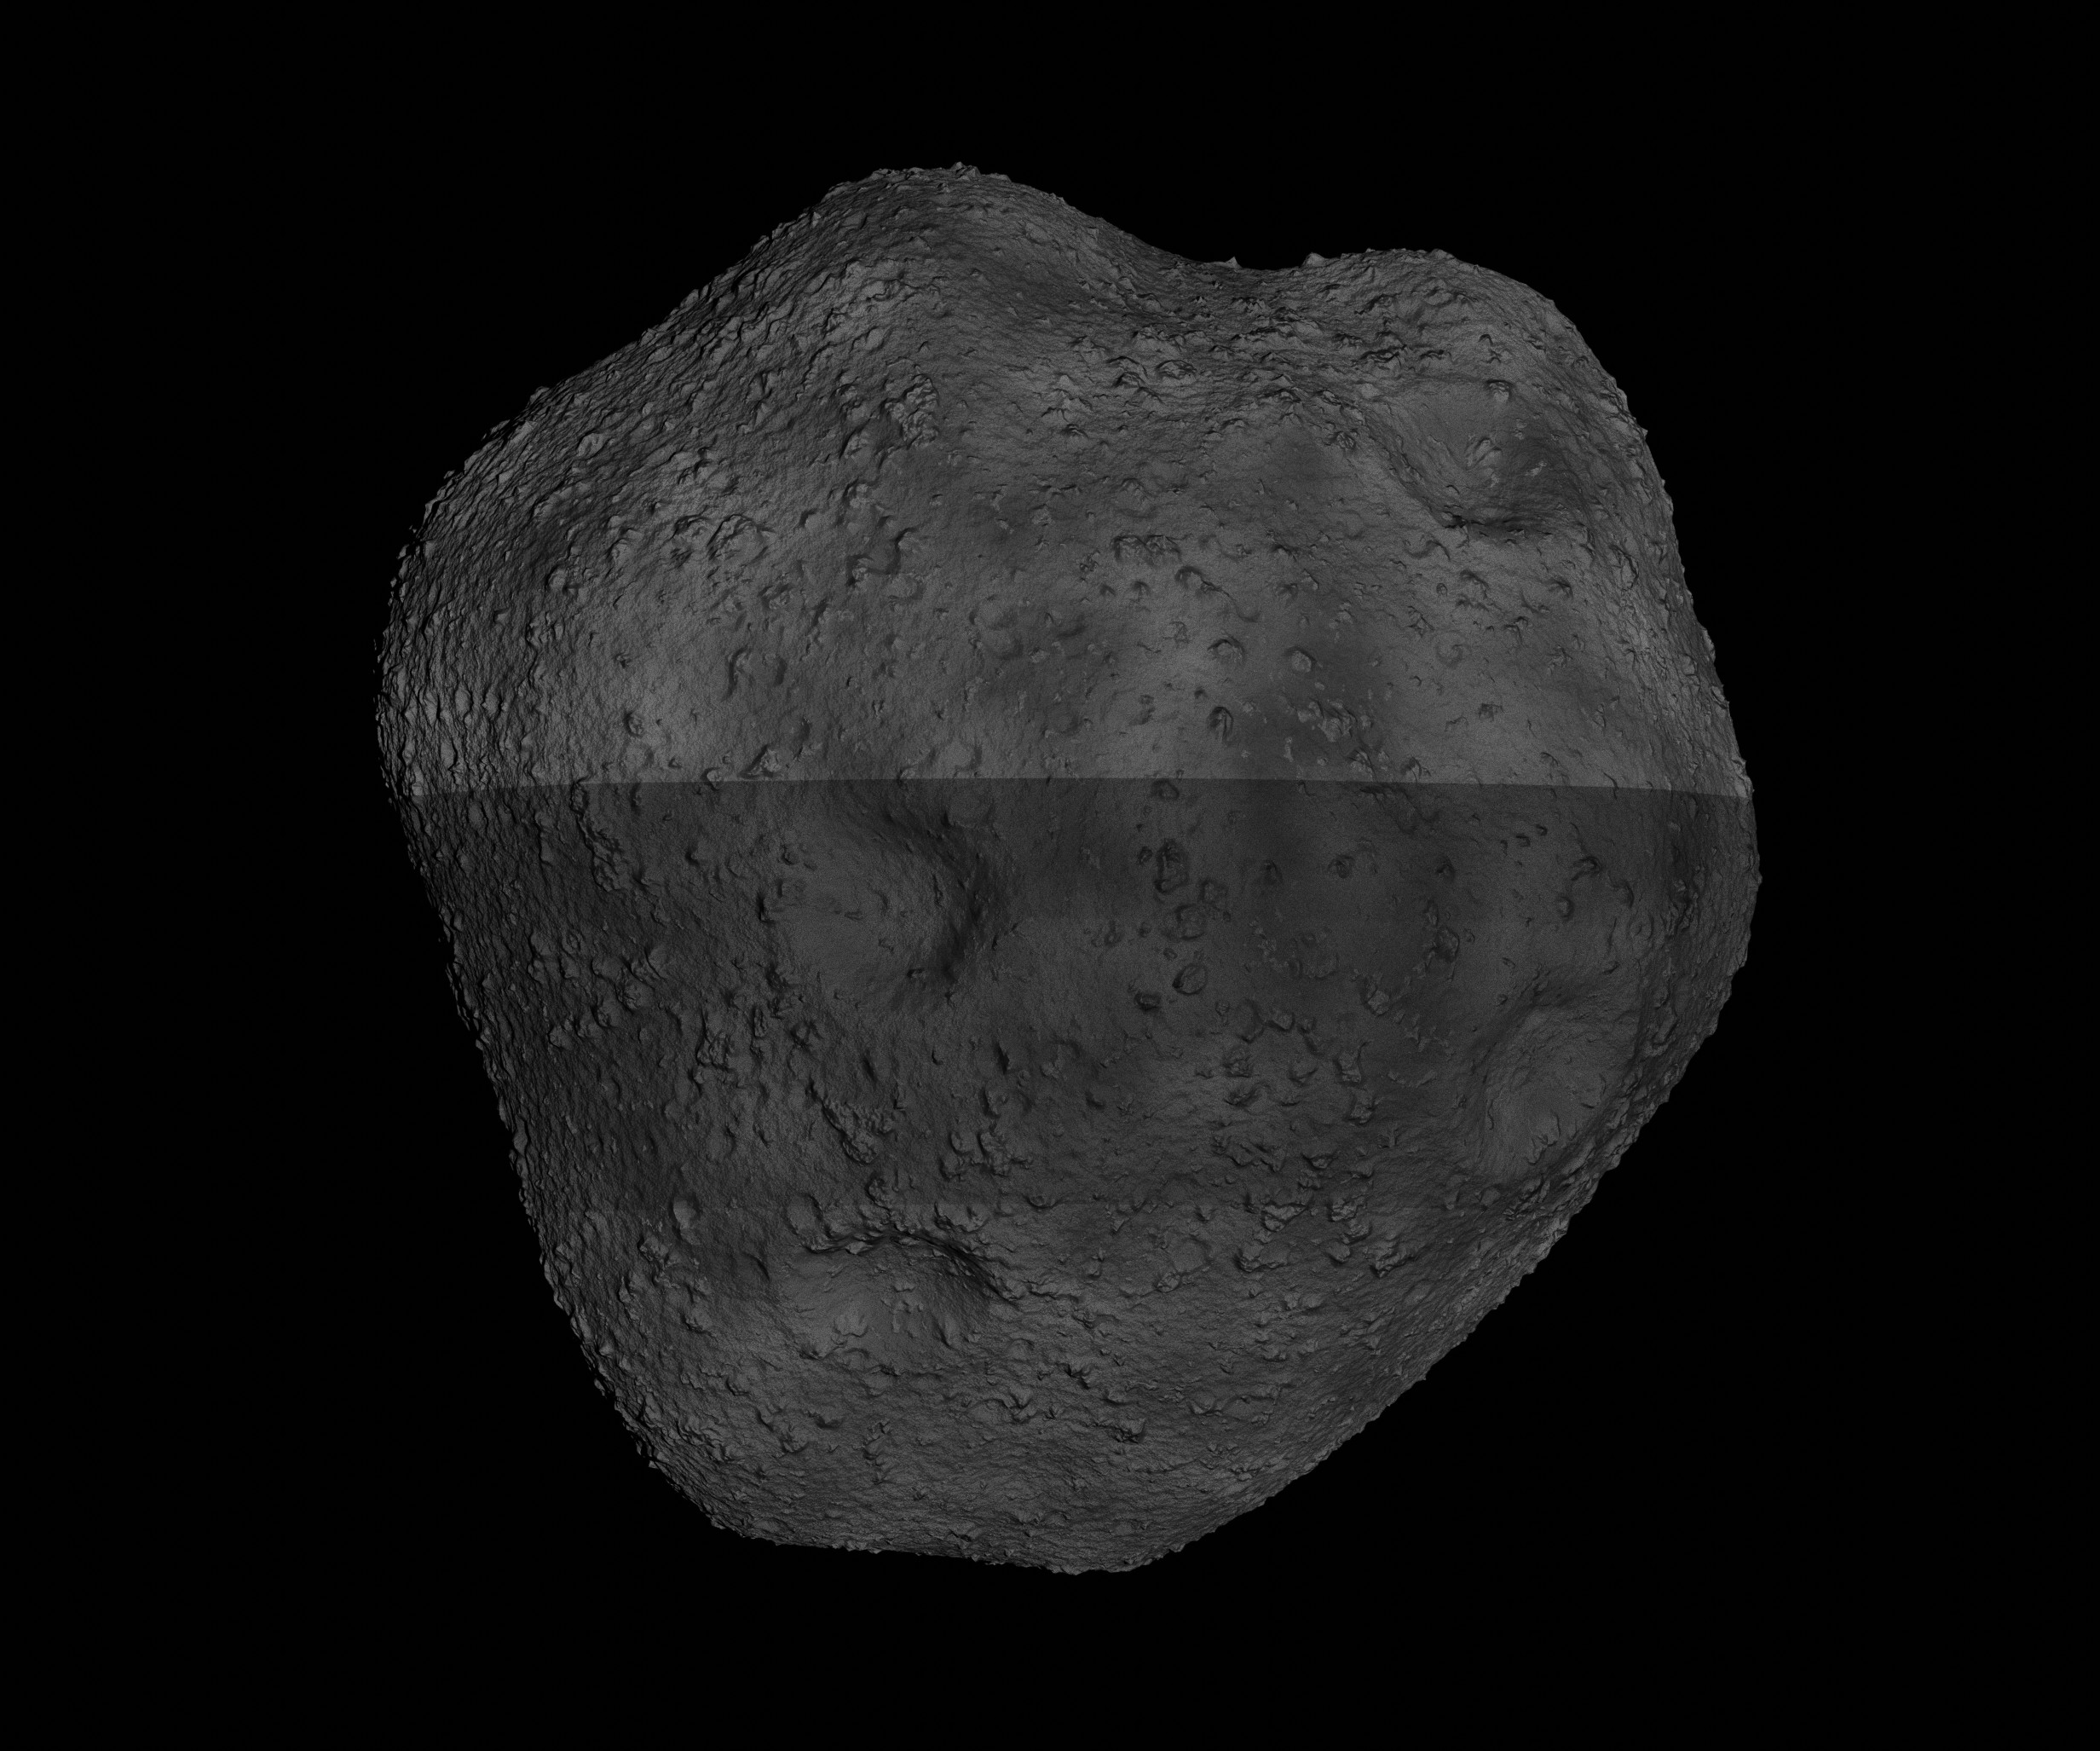
\includegraphics[width=\textwidth]{doc/thesis/0_figures/rendering_artefacts/400_10_SssbOnly_2017-08-15T115845-190000.jpg}
            \caption{\SI{400}{\kilo\meter}.}
            \label{fig:render_artefacts_400}
        \end{subfigure}
    \caption{Surface of a \SI{10}{\kilo\meter} \gls{sssb} for flybys with the given closest approach distance. Rendering artefacts, the stripes, are clearly visible in all three images.}
    \label{fig:render_artefacts}
\end{figure}

A second problem occurred in a scenario with \SI{50}{\kilo\meter} minimum distance and a \SI{1}{\kilo\meter} \gls{sssb}. A single image was found to be darker than all other images in the data set. A series of three images is shown in Figure~\ref{fig:render_dark}, with the middle image being darker despite one small patch of pixels. In total, three pixels are much brighter than any other pixel in the image. These are so-called \textit{fireflies}~\cite{Valenza2015BlenderCookbook}. Figure~\ref{fig:render_dark} contains composed images for better visibility of the artefact. However, the artefact also exists in the raw image hence it is a rendering artefact and not introduced by the composition process. No second image with the same issue was found in any other data set therefore the problem was not investigated further.

\begin{figure}[htb]
    \centering
        \begin{subfigure}[b]{0.32\textwidth}
            \centering
            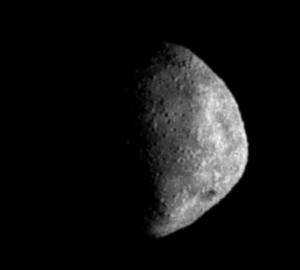
\includegraphics[width=\textwidth]{doc/thesis/0_figures/composition_darkening/50km_Inst_2017-08-15T115816-993000_center.png}
            \label{fig:render_dark_1}
        \end{subfigure}
        \begin{subfigure}[b]{0.32\textwidth}
            \centering
            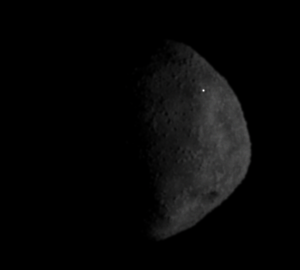
\includegraphics[width=\textwidth]{doc/thesis/0_figures/composition_darkening/Inst_2017-08-15T115818-000000_center.png}
            \label{fig:render_dark_2}
        \end{subfigure}
        \begin{subfigure}[b]{0.32\textwidth}
            \centering
            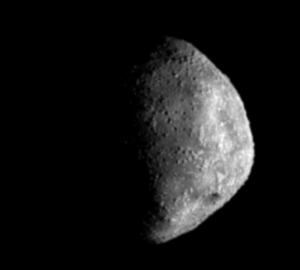
\includegraphics[width=\textwidth]{doc/thesis/0_figures/composition_darkening/Inst_2017-08-15T115819-007000_center.png}
            \label{fig:render_dark_3}
        \end{subfigure}
    \caption{Darkening of overall \gls{sssb} body due to three pixel being much brighter, also referred to as fireflies. All three images are composed images for better visibility of the artefact. The images are cropped to show the \gls{sssb} nucleus up close.}
    \label{fig:render_dark}
\end{figure}

\subsection{Compression} \label{sec:results_comp}
The \gls{sispo} software package was used to study the effects of compression in different scenarios. The scenarios are presented in Table~\ref{tab:sim_params}. Two compression algorithms were used to study compression effects. The \gls{png} format was used because of its wide support among different software packages and \gls{jp2}. Scenarios with varying \gls{sssb} nucleus sizes and flyby distance were simulated. 
Comparison of the different compression algorithms is based on several output parameters. The data size of the compressed image series, the number of points in the dense reconstructed point cloud, the number of vertices and the number of faces of the refined reconstructed model. These outputs relate well to the level of detail of the rendered images, since \gls{sfm} algorithms rely on surface details for reconstruction.

\begin{table}[htb]
    \centering
    \caption{Simulation parameters used for investigating capabilities of \gls{sispo}. For each scenario \gls{png}, \gls{jp2} quality 1000, quality 100, quality 10 and quality 1 compression methods were used to investigate the effects of compression.}
    \label{tab:sim_params}
    \begin{tabular}{l|lll}
        Scenario ID  & \gls{sssb} Size \SI{}{\kilo\meter} & Encounter Distance \SI{}{\kilo\meter} & Number of Images \\ \hline
        1 & 1  & 50  & 120\\
        2 & 1  & 100 & 120\\
        3 & 1  & 200 & 120\\
        4 & 1  & 400 & 120\\
        5 & 1  & 50  & 30\\
        6 & 1  & 100 & 30\\
        7 & 1  & 200 & 30\\
        8 & 1  & 400 & 30\\
        9 & 10 & 50  & 30\\
    \end{tabular}
\end{table}

\subsubsection{Image Quality Comparison} \label{sec:img_quali_comp}
To compare the image quality after different levels of compression, a specific image is selected which is compressed to different levels. Since reconstruction is mostly influenced by surface features, a scene with a distance of \SI{50}{\kilo\meter} was selected for comparison. To better show the artefacts created by compression, the highlighted area in Figure~\ref{fig:img_quality_frame} was studied up closer.

\begin{figure}[htb]
    \centering
    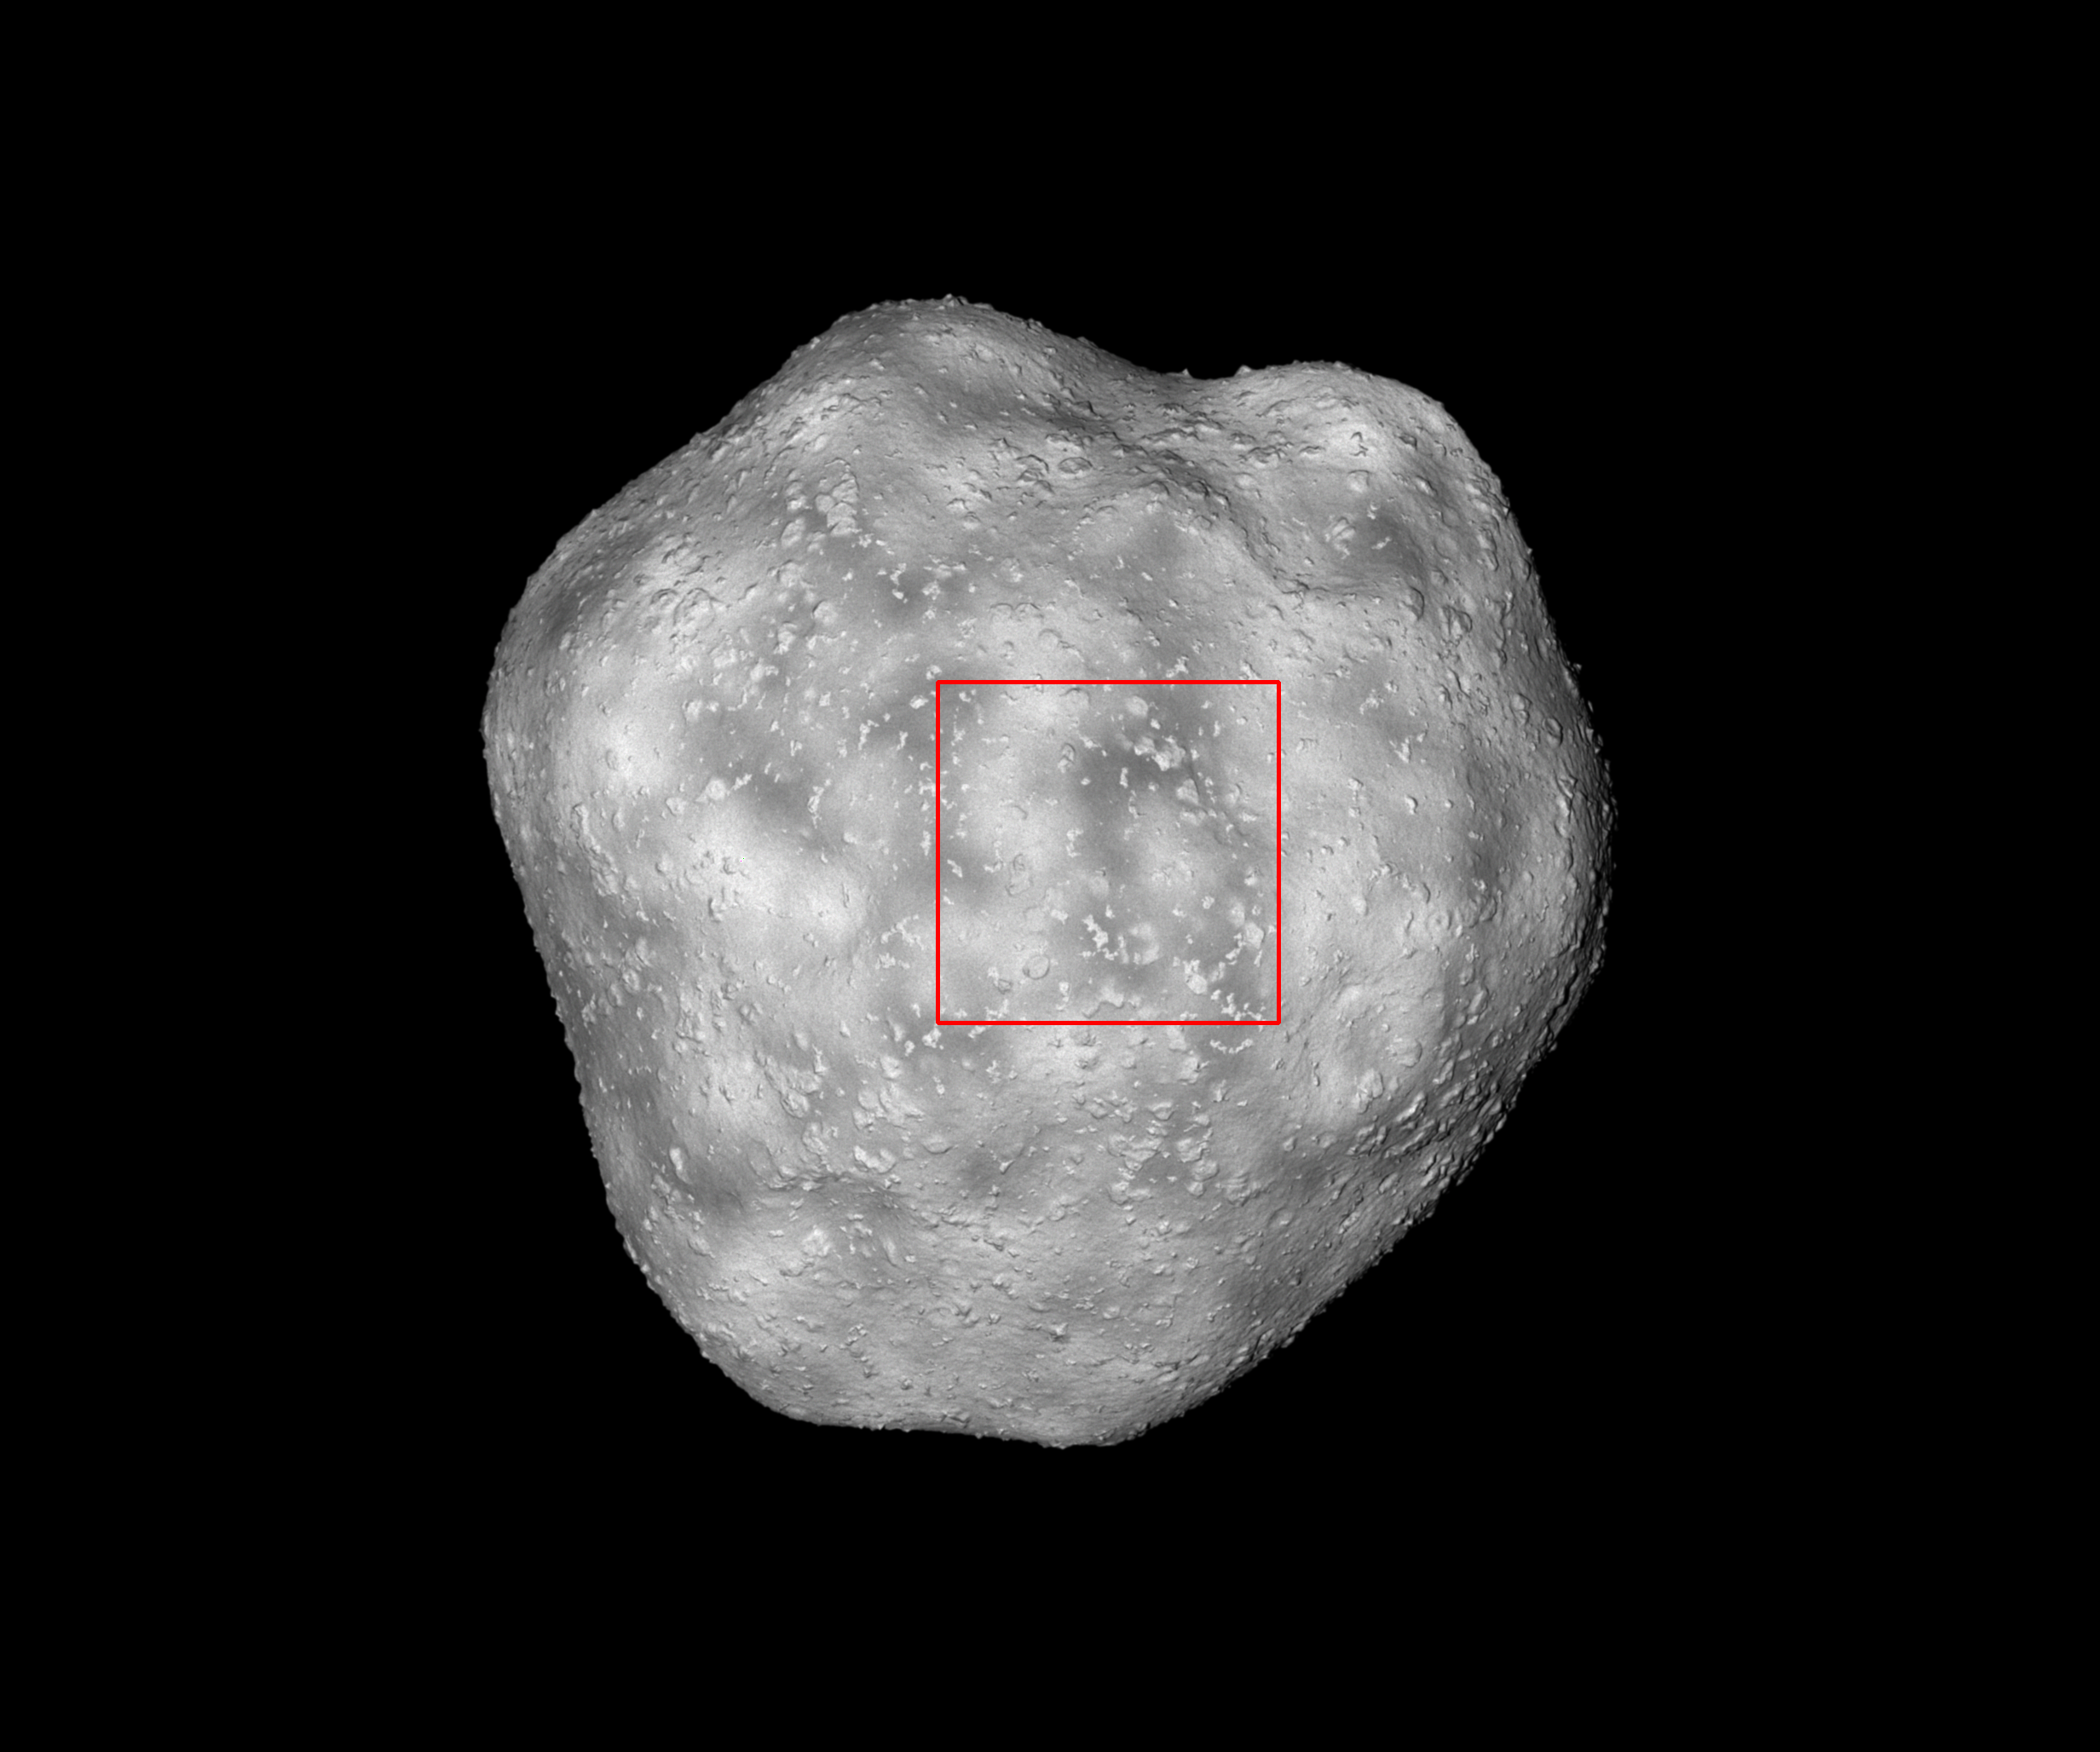
\includegraphics[width=.7\textwidth]{doc/thesis/0_figures/compare_quality/set1/jp2_1000_frame.png}
    \caption{Scene used for quality comparison. Highlighted in red is the area studied up closer. The specific area was selected since it includes a wide range of colours and various sized surface features.}
    \label{fig:img_quality_frame}
\end{figure}

Figure~\ref{fig:img_quality_comp} shows series of close-up views of rendered images at different levels of compression and one \gls{png} image as reference. The high quality level images do not show any difference to the \gls{png} image. Figure~\ref{fig:img_quality_5} shows a minor visible difference to the lossless compressed image. Only image~\ref{fig:img_quality_1} contains clearly visible compression artefacts.
\begin{figure}[htb]
    \centering
        \begin{subfigure}[b]{0.44\textwidth}
            \centering
            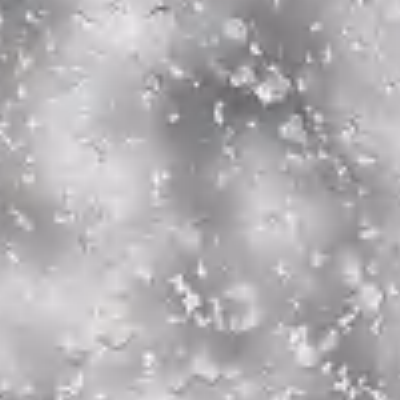
\includegraphics[width=\textwidth]{doc/thesis/0_figures/compare_quality/set1/jp2_1_center.png}
            \caption{\gls{jp2} quality 1.}
            \label{fig:img_quality_1}
        \end{subfigure}
        \begin{subfigure}[b]{0.44\textwidth}
            \centering
            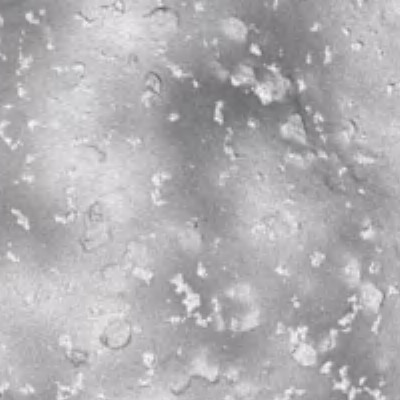
\includegraphics[width=\textwidth]{doc/thesis/0_figures/compare_quality/set1/jp2_5_center.png}
            \caption{\gls{jp2} quality 5.}
            \label{fig:img_quality_5}
        \end{subfigure}
        \\
        \begin{subfigure}[b]{0.44\textwidth}
            \centering
            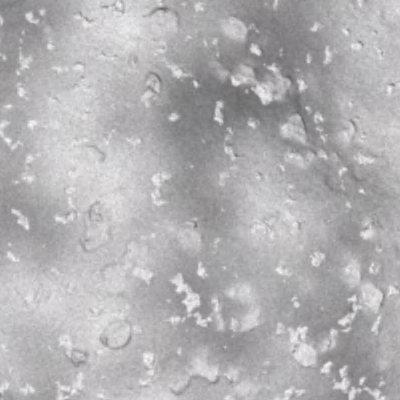
\includegraphics[width=\textwidth]{doc/thesis/0_figures/compare_quality/set1/jp2_10_center.png}
            \caption{\gls{jp2} quality 10.}
            \label{fig:img_quality_10}
        \end{subfigure}
        \begin{subfigure}[b]{0.44\textwidth}
            \centering
            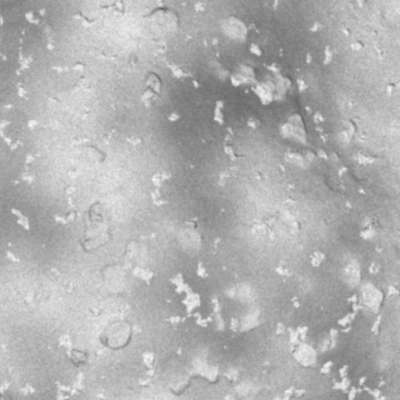
\includegraphics[width=\textwidth]{doc/thesis/0_figures/compare_quality/set1/jp2_100_center.png}
            \caption{\gls{jp2} quality 100.}
            \label{fig:img_quality_100}
        \end{subfigure}
        \\
        \begin{subfigure}[b]{0.44\textwidth}
            \centering
            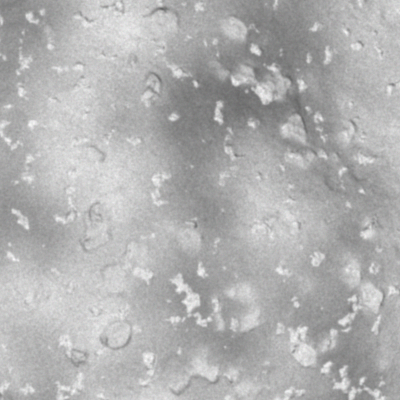
\includegraphics[width=\textwidth]{doc/thesis/0_figures/compare_quality/set1/jp2_1000_center.png}
            \caption{\gls{jp2} quality 1000.}
            \label{fig:img_quality_1000}
        \end{subfigure}
        \begin{subfigure}[b]{0.44\textwidth}
            \centering
            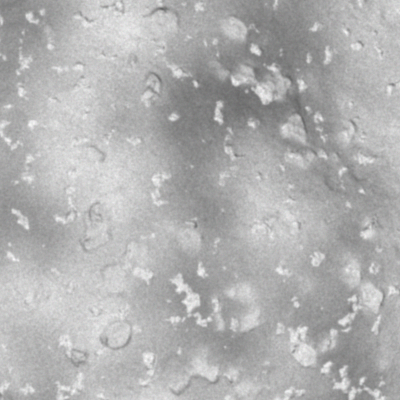
\includegraphics[width=\textwidth]{doc/thesis/0_figures/compare_quality/set1/png_center.png}
            \caption{\gls{png}}
            \label{fig:img_quality_png}
        \end{subfigure}
    \caption{Close-up images with different level of compression using \gls{jp2} and one \gls{png}.}
    \label{fig:img_quality_comp}
\end{figure}

Difference images and histograms are used to further investigate the effects of compression further. Difference images take the L2-norm of the \gls{rgb} values of each pixel and subtract them from the respective value of the \gls{png} image. The result is a difference image showing the L2-norm differences through a colour scale. For the histograms the zero values were removed to only show differences. Therefore, the total number of pixels and the percentage compared to the original that were used for the histogram are given as well. Difference images and histograms are analysed for the overall image in Figure~\ref{fig:img_quality_frame} and for the highlighted area. The overall difference images and their histograms are shown in Figures~\ref{fig:img_quality_heatmap} and \ref{fig:img_quality_histogram} respectively. The difference images and their histograms for the close-ups are shown in Figures~\ref{fig:img_quality_center_heatmap} and \ref{fig:img_quality_center_histogram}.

\begin{figure}[htb]
    \centering
        \begin{subfigure}[b]{0.49\textwidth}
            \centering
            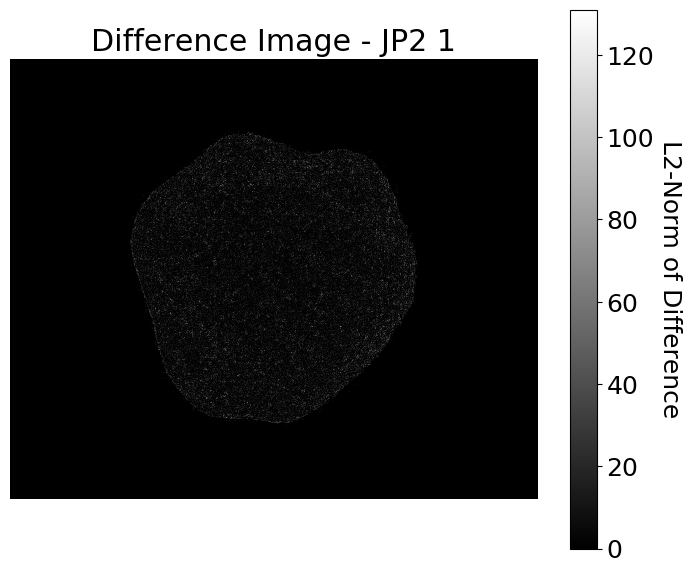
\includegraphics[width=\textwidth]{doc/thesis/0_figures/compare_quality/set1/jp2_1_diff_heatmap.png}
            \caption{\gls{jp2} quality 1.}
            \label{fig:img_quality_heatmap_1}
        \end{subfigure}
        \begin{subfigure}[b]{0.49\textwidth}
            \centering
            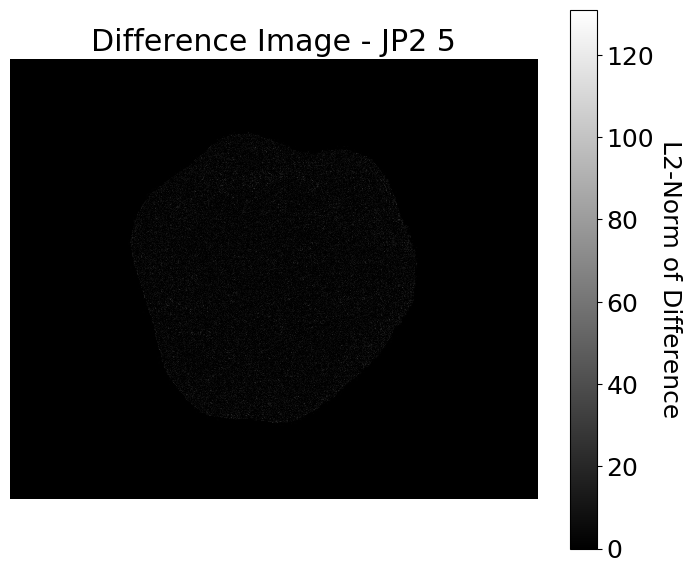
\includegraphics[width=\textwidth]{doc/thesis/0_figures/compare_quality/set1/jp2_5_diff_heatmap.png}
            \caption{\gls{jp2} quality 5.}
            \label{fig:img_quality_heatmap_5}
        \end{subfigure}
        \\
        \begin{subfigure}[b]{0.49\textwidth}
            \centering
            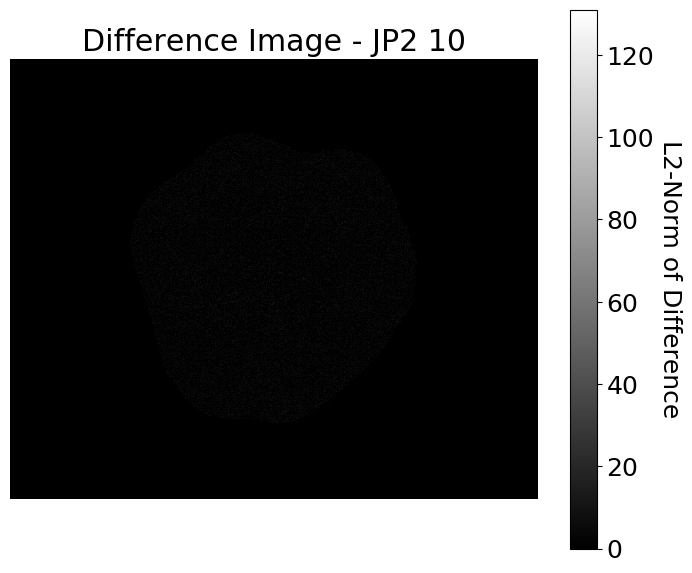
\includegraphics[width=\textwidth]{doc/thesis/0_figures/compare_quality/set1/jp2_10_diff_heatmap.png}
            \caption{\gls{jp2} quality 10.}
            \label{fig:img_quality_heatmap_10}
        \end{subfigure}
        \begin{subfigure}[b]{0.49\textwidth}
            \centering
            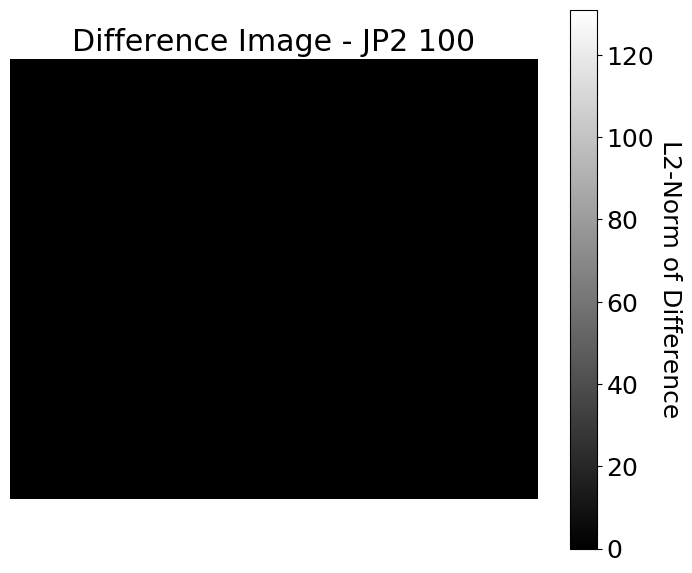
\includegraphics[width=\textwidth]{doc/thesis/0_figures/compare_quality/set1/jp2_100_diff_heatmap.png}
            \caption{\gls{jp2} quality 100.}
            \label{fig:img_quality_heatmap_100}
        \end{subfigure}
        \\
        \begin{subfigure}[b]{0.49\textwidth}
            \centering
            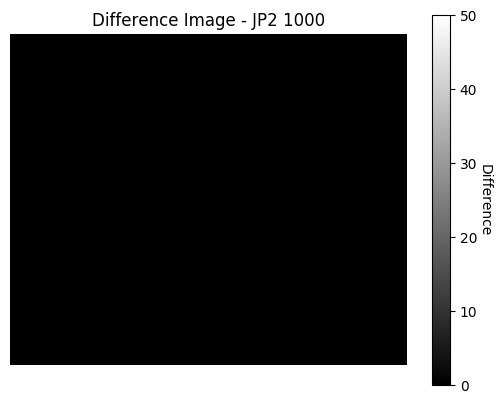
\includegraphics[width=\textwidth]{doc/thesis/0_figures/compare_quality/set1/jp2_1000_diff_heatmap.png}
            \caption{\gls{jp2} quality 1000.}
            \label{fig:img_quality_heatmap_1000}
        \end{subfigure}
        \begin{subfigure}[b]{0.49\textwidth}
            \centering
            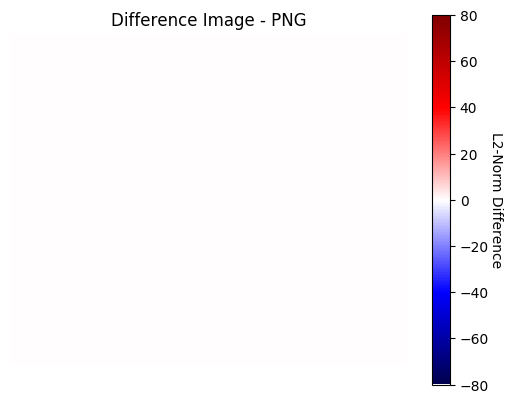
\includegraphics[width=\textwidth]{doc/thesis/0_figures/compare_quality/set1/png_diff_heatmap.png}
            \caption{\gls{png}}
            \label{fig:img_quality_heatmap_png}
        \end{subfigure}
    \caption{Difference images of overall images with varying levels of compression using \gls{jp2} and one \gls{png}.}
    \label{fig:img_quality_heatmap}
\end{figure}

\begin{figure}[htb]
    \centering
        \begin{subfigure}[b]{0.49\textwidth}
            \centering
            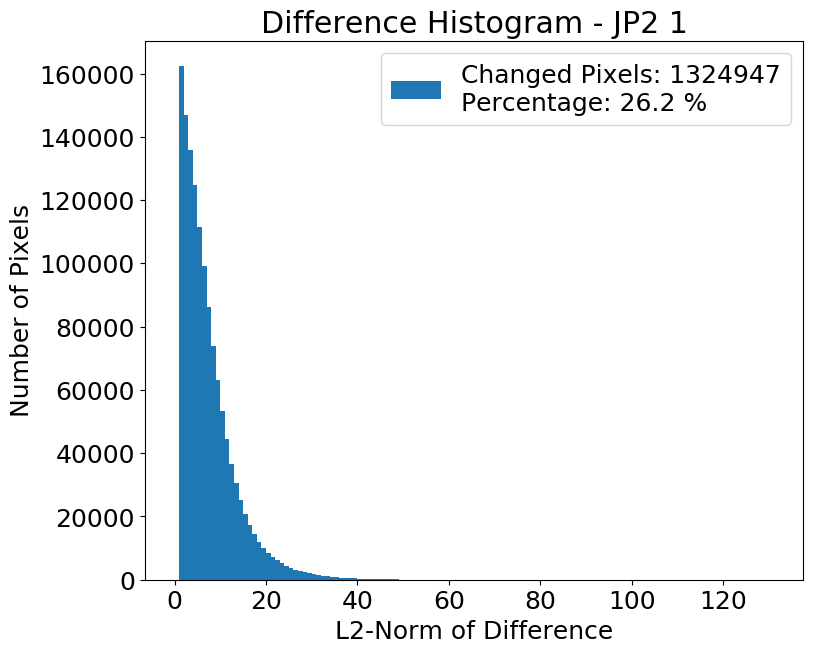
\includegraphics[width=\textwidth]{doc/thesis/0_figures/compare_quality/set1/jp2_1_diff_histogram.png}
            \caption{\gls{jp2} quality 1.}
            \label{fig:img_quality_histogram_1}
        \end{subfigure}
        \begin{subfigure}[b]{0.49\textwidth}
            \centering
            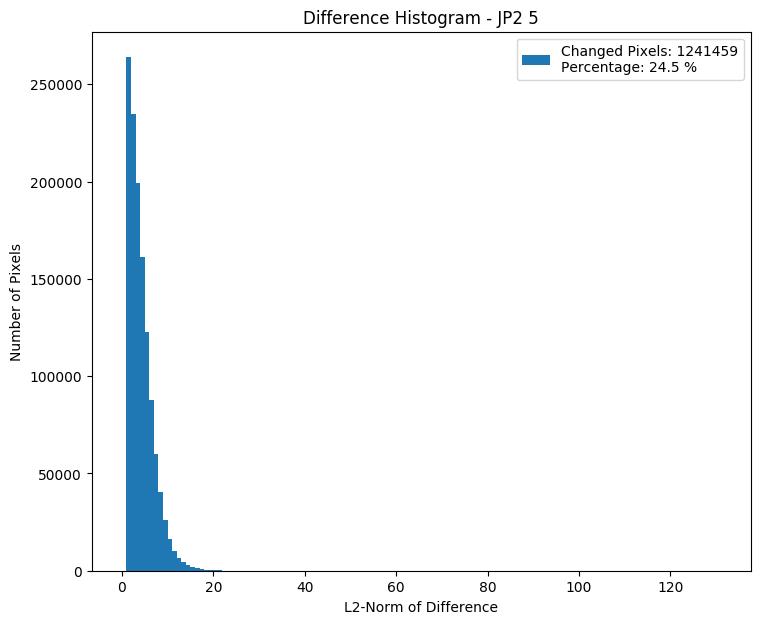
\includegraphics[width=\textwidth]{doc/thesis/0_figures/compare_quality/set1/jp2_5_diff_histogram.png}
            \caption{\gls{jp2} quality 5.}
            \label{fig:img_quality_histogram_5}
        \end{subfigure}
        \\
        \begin{subfigure}[b]{0.49\textwidth}
            \centering
            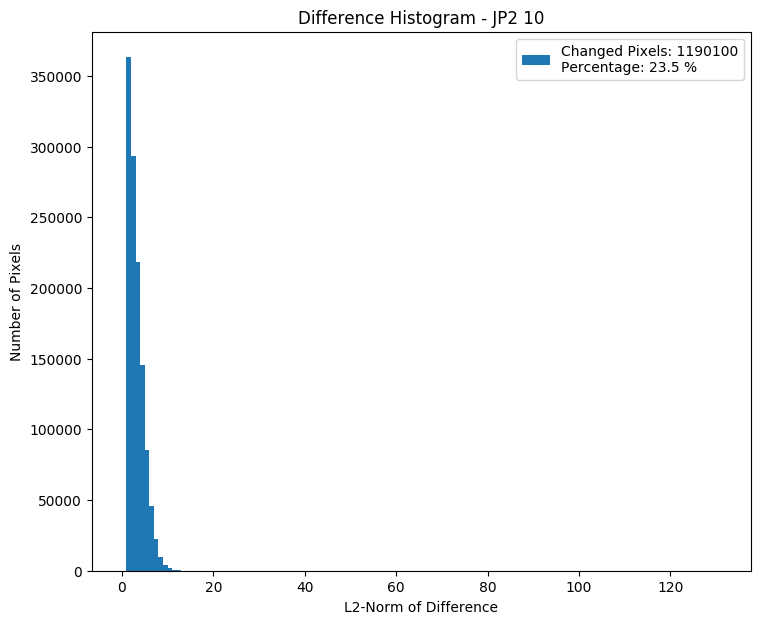
\includegraphics[width=\textwidth]{doc/thesis/0_figures/compare_quality/set1/jp2_10_diff_histogram.png}
            \caption{\gls{jp2} quality 10.}
            \label{fig:img_quality_histogram_10}
        \end{subfigure}
        \begin{subfigure}[b]{0.49\textwidth}
            \centering
            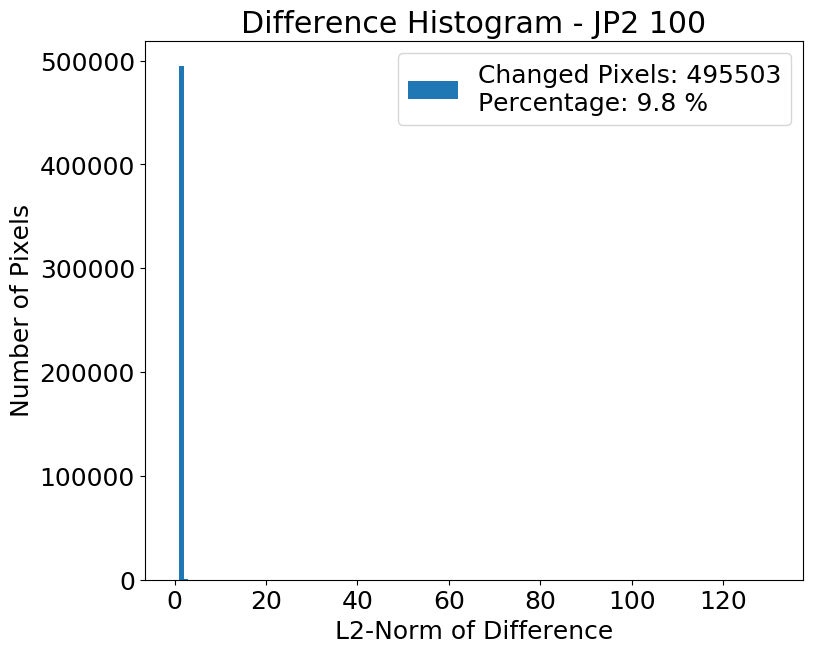
\includegraphics[width=\textwidth]{doc/thesis/0_figures/compare_quality/set1/jp2_100_diff_histogram.png}
            \caption{\gls{jp2} quality 100.}
            \label{fig:img_quality_histogram_100}
        \end{subfigure}
        \\
        \begin{subfigure}[b]{0.49\textwidth}
            \centering
            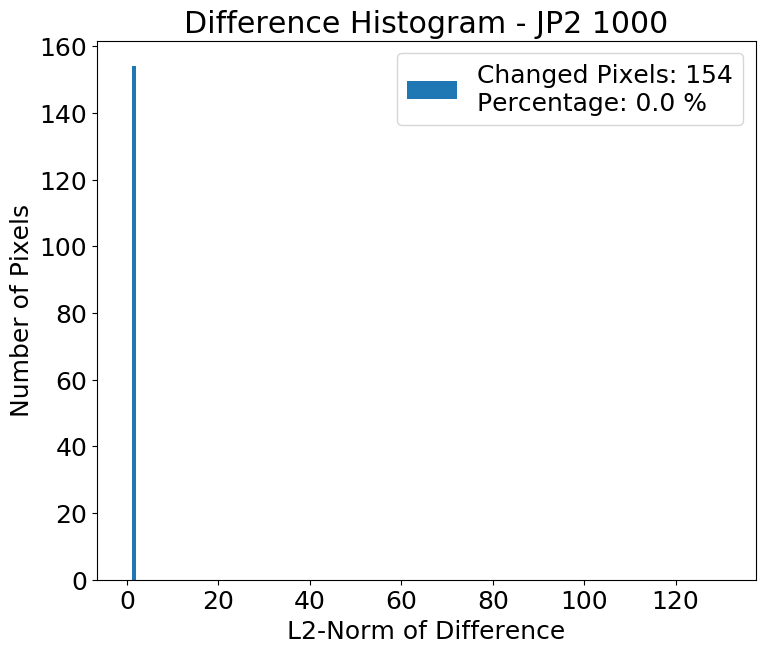
\includegraphics[width=\textwidth]{doc/thesis/0_figures/compare_quality/set1/jp2_1000_diff_histogram.png}
            \caption{\gls{jp2} quality 1000.}
            \label{fig:img_quality_histogram_1000}
        \end{subfigure}
        \begin{subfigure}[b]{0.49\textwidth}
            \centering
            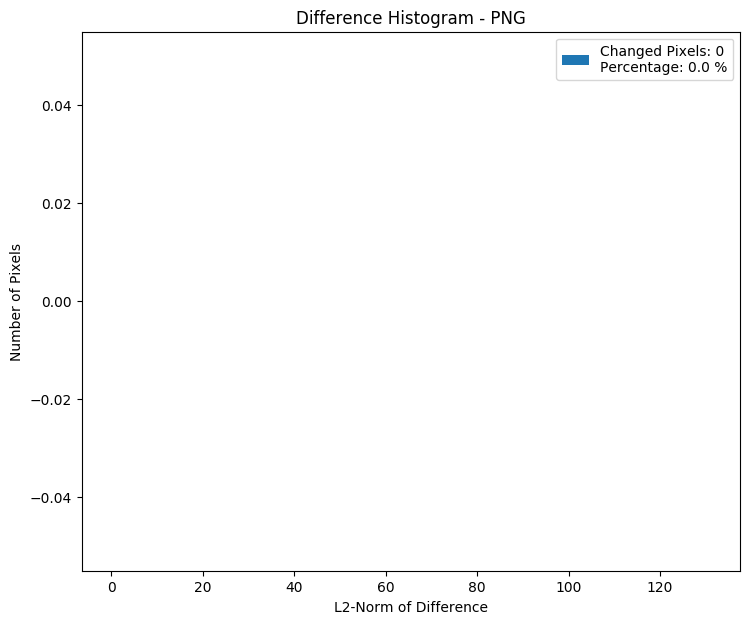
\includegraphics[width=\textwidth]{doc/thesis/0_figures/compare_quality/set1/png_diff_histogram.png}
            \caption{\gls{png}}
            \label{fig:img_quality_histogram_png}
        \end{subfigure}
    \caption{Histograms of overall difference images with varying levels of compression using \gls{jp2} and one \gls{png}.}
    \label{fig:img_quality_histogram}
\end{figure}

\begin{figure}[htb]
    \centering
        \begin{subfigure}[b]{0.49\textwidth}
            \centering
            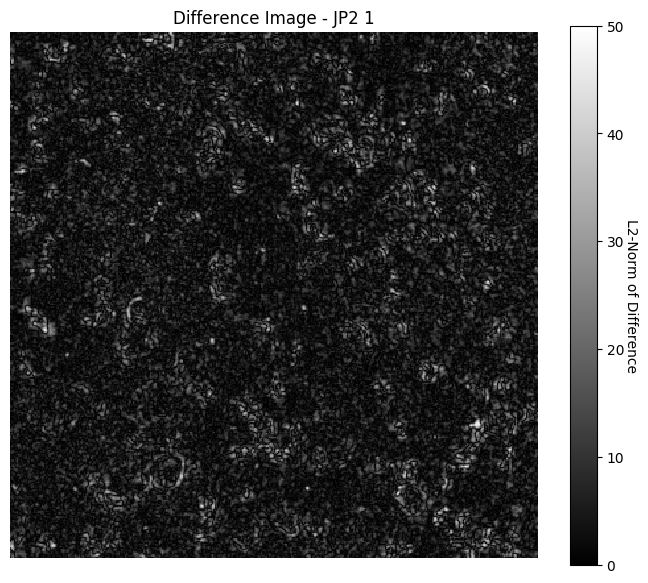
\includegraphics[width=\textwidth]{doc/thesis/0_figures/compare_quality/set1/jp2_1_center_diff_heatmap.png}
            \caption{\gls{jp2} quality 1.}
            \label{fig:img_quality_center_heatmap_1}
        \end{subfigure}
        \begin{subfigure}[b]{0.49\textwidth}
            \centering
            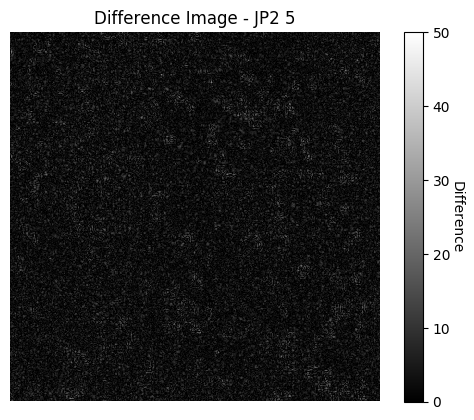
\includegraphics[width=\textwidth]{doc/thesis/0_figures/compare_quality/set1/jp2_5_center_diff_heatmap.png}
            \caption{\gls{jp2} quality 5.}
            \label{fig:img_quality_center_heatmap_5}
        \end{subfigure}
        \\
        \begin{subfigure}[b]{0.49\textwidth}
            \centering
            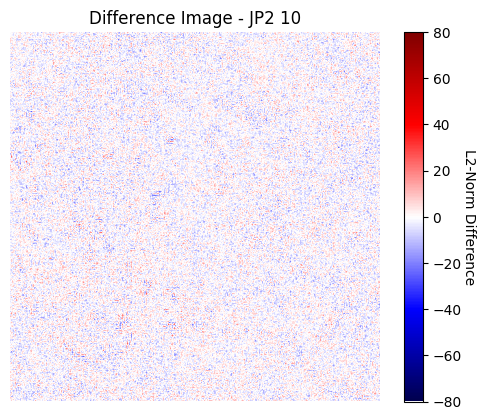
\includegraphics[width=\textwidth]{doc/thesis/0_figures/compare_quality/set1/jp2_10_center_diff_heatmap.png}
            \caption{\gls{jp2} quality 10.}
            \label{fig:img_quality_center_heatmap_10}
        \end{subfigure}
        \begin{subfigure}[b]{0.49\textwidth}
            \centering
            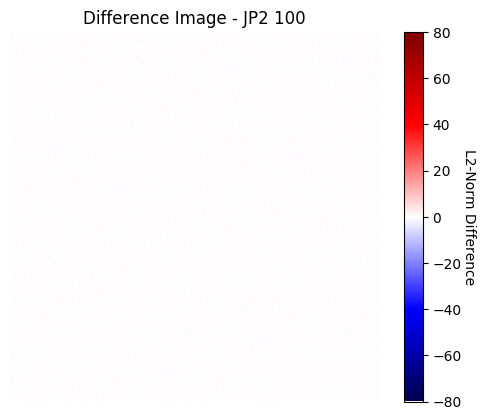
\includegraphics[width=\textwidth]{doc/thesis/0_figures/compare_quality/set1/jp2_100_center_diff_heatmap.png}
            \caption{\gls{jp2} quality 100.}
            \label{fig:img_quality_center_heatmap_100}
        \end{subfigure}
        \\
        \begin{subfigure}[b]{0.49\textwidth}
            \centering
            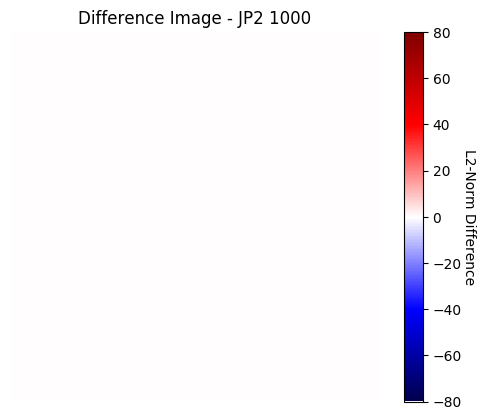
\includegraphics[width=\textwidth]{doc/thesis/0_figures/compare_quality/set1/jp2_1000_center_diff_heatmap.png}
            \caption{\gls{jp2} quality 1000.}
            \label{fig:img_quality_center_heatmap_1000}
        \end{subfigure}
        \begin{subfigure}[b]{0.49\textwidth}
            \centering
            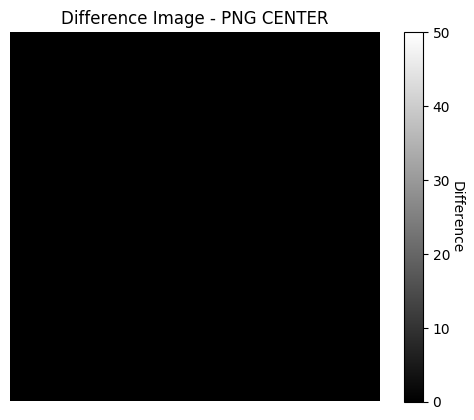
\includegraphics[width=\textwidth]{doc/thesis/0_figures/compare_quality/set1/png_center_diff_heatmap.png}
            \caption{\gls{png}}
            \label{fig:img_quality_center_heatmap_png}
        \end{subfigure}
    \caption{Difference images of close-ups with varying levels of compression using \gls{jp2} and one \gls{png}.}
    \label{fig:img_quality_center_heatmap}
\end{figure}

\begin{figure}[htb]
    \centering
        \begin{subfigure}[b]{0.49\textwidth}
            \centering
            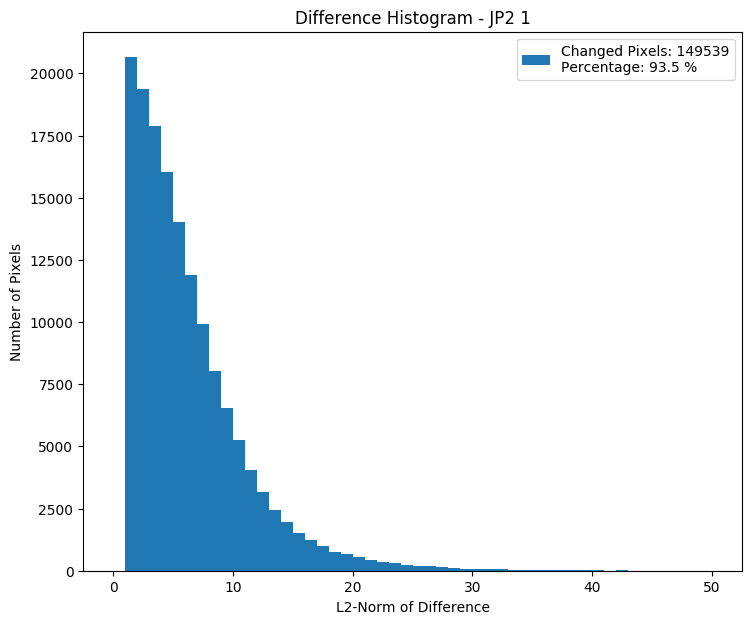
\includegraphics[width=\textwidth]{doc/thesis/0_figures/compare_quality/set1/jp2_1_center_diff_histogram.png}
            \caption{\gls{jp2} quality 1.}
            \label{fig:img_quality_center_histogram_1}
        \end{subfigure}
        \begin{subfigure}[b]{0.49\textwidth}
            \centering
            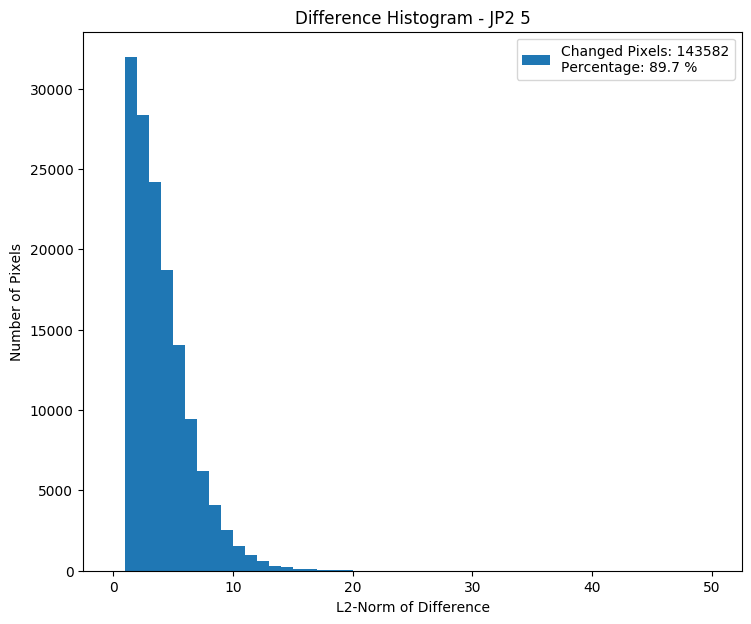
\includegraphics[width=\textwidth]{doc/thesis/0_figures/compare_quality/set1/jp2_5_center_diff_histogram.png}
            \caption{\gls{jp2} quality 5.}
            \label{fig:img_quality_center_histogram_5}
        \end{subfigure}
        \\
        \begin{subfigure}[b]{0.49\textwidth}
            \centering
            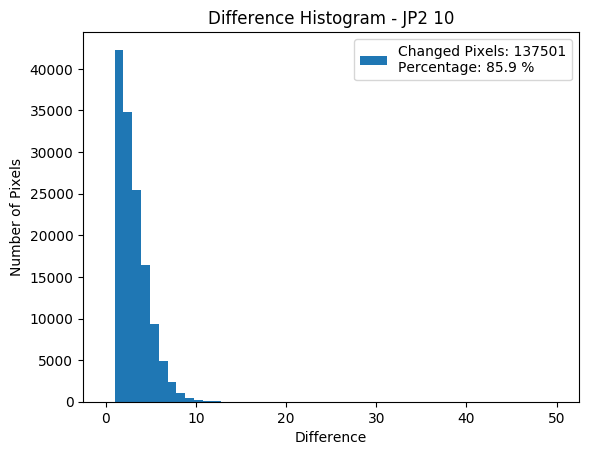
\includegraphics[width=\textwidth]{doc/thesis/0_figures/compare_quality/set1/jp2_10_center_diff_histogram.png}
            \caption{\gls{jp2} quality 10.}
            \label{fig:img_quality_center_histogram_10}
        \end{subfigure}
        \begin{subfigure}[b]{0.49\textwidth}
            \centering
            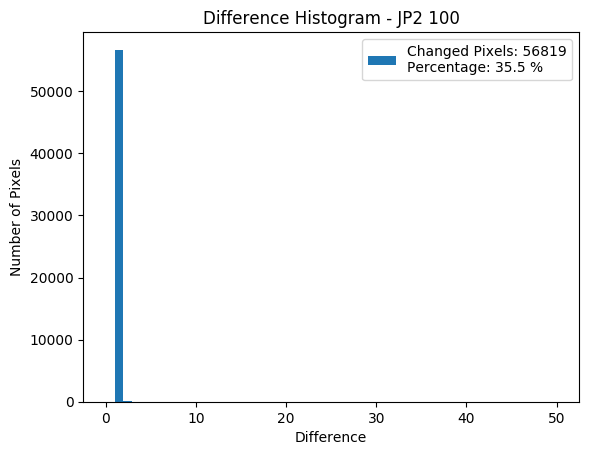
\includegraphics[width=\textwidth]{doc/thesis/0_figures/compare_quality/set1/jp2_100_center_diff_histogram.png}
            \caption{\gls{jp2} quality 100.}
            \label{fig:img_quality_center_histogram_100}
        \end{subfigure}
        \\
        \begin{subfigure}[b]{0.49\textwidth}
            \centering
            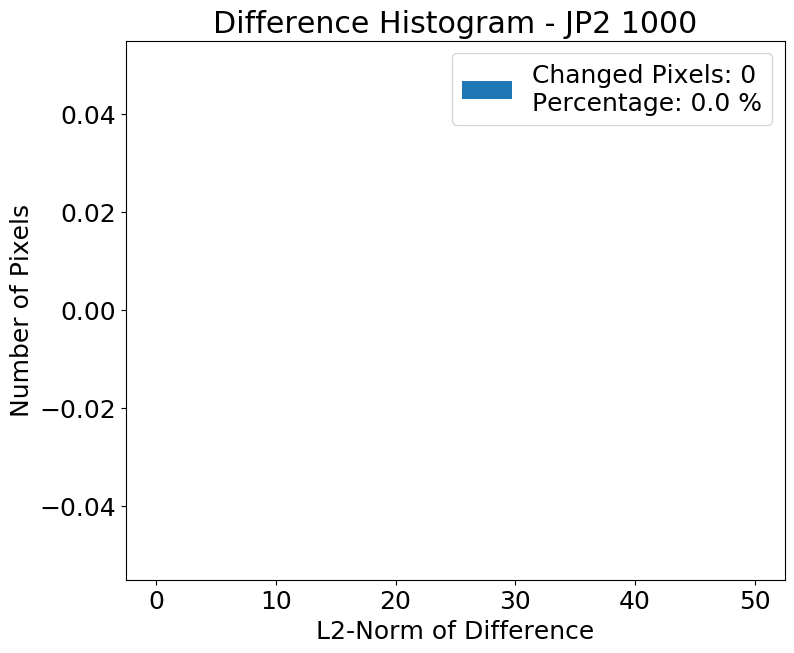
\includegraphics[width=\textwidth]{doc/thesis/0_figures/compare_quality/set1/jp2_1000_center_diff_histogram.png}
            \caption{\gls{jp2} quality 1000.}
            \label{fig:img_quality_center_histogram_1000}
        \end{subfigure}
        \begin{subfigure}[b]{0.49\textwidth}
            \centering
            \includegraphics[width=\textwidth]{doc/thesis/0_figures/compare_quality/set1/png_center_diff_histogram.png}
            \caption{\gls{png}}
            \label{fig:img_quality_center_histogram_png}
        \end{subfigure}
    \caption{Histograms of close-up difference images with varying levels of compression using \gls{jp2} and one \gls{png}. All images use the same color scale, making image \ref{fig:img_quality_center_histogram_100} look entirely white.}
    \label{fig:img_quality_center_histogram}
\end{figure}

The difference images for \gls{png} as well as their histograms are empty figures as expected since the \gls{png} image is the base line. Also the difference images for quality levels 100 and 1000 seem completely white, however the histograms reveal that there is a small number of pixels that were altered. 
Starting from quality level 10 and lower, compression starts having effect on the image quality. Generally, with lowering image quality the number of altered points and the magnitude of alteration increase as expected. Also, the effect of compression is stronger on the close-up images than on the overall images. This can be explained by the large black portion in these images since no stars are visible in the background due to short exposure times. For the overall images in Figures~\ref{fig:img_quality_heatmap_1}, \ref{fig:img_quality_heatmap_5} and \ref{fig:img_quality_heatmap_10} the differences resemble random noise. Difference images using varying scales for the same data set are shown in Appendix~\ref{sec:image_differences} revealing that the quality 100 image also resembles random noise. The histograms in Figures~\ref{fig:img_quality_histogram_1}, \ref{fig:img_quality_histogram_5} and \ref{fig:img_quality_histogram_10} show that the differences create a Gaussian distribution. While the histograms for the overall images and the close-ups have similar shapes, the difference images show a distinct difference. The overall difference images resemble random noise while the close-up images show some structures. In comparably flat areas the close-up difference images resemble white noise as well, however around surface features like boulders, the feature contours are clearly visible in the difference images meaning that the contours of these features are altered stronger than featureless areas.
The histograms in Figure~\ref{fig:img_quality_histogram_1}, \ref{fig:img_quality_histogram_5}, \ref{fig:img_quality_center_histogram_1} and \ref{fig:img_quality_center_histogram_5} seem to have more values below zero than above zero. A negative value reflects a higher value for the \gls{jp2} image compared to the \gls{png} image. It seems that images compressed with \gls{jp2} tend to become brighter since the L2-norm of \gls{rgb} values relates to brightness.

\subsection{Reconstruction}
\gls{sispo} reconstructs using default parameters given in Table~\ref{tab:comp_settings}. \textit{refine\_options} is set to NONE to make \gls{sfm} algorithms more likely to converge. Camera calibration as described in Section~\ref{sec:t_cv} is not needed since in space missions, the intrinsic camera parameters can be determined with sufficient accuracy before launch and therefore the parameters do not need to be optimised anymore.

\begin{table}[htb]
    \centering
    \caption{Reconstruction Settings}
    \label{tab:comp_settings}
    \begin{tabular}{l|l}
        \textbf{Parameter Name} & \textbf{Value} \\ \hline
        export\_type       & obj   \\
        focal & 66667 \\
        cam\_model & \SI{1}{}     \\
        geo\_model & \SI{10}{\kilo\meter\per\second} \\
        num\_overlaps  & \SI{4}{} \\
        use\_prior & \SI{1}{} \\
        use\_upright & \SI{0}{} \\
        force\_compute & \SI{0}{} \\
        descriptor & SIFT \\
        d\_preset & ULTRA \\
        method & FASTCASCADEHASHINGL2 \\
        refine\_options & NONE \\
        reduce\_memory & 1
    \end{tabular}
\end{table}

\gls{sispo} is choosing which result of which reconstruction method to use based on the number of reconstructed points. Comparing the chosen algorithm with the input parameter reveals that the first incremental \gls{sfm} reconstruction performs better when the flyby distance is smaller while the second incremental \gls{sfm} algorithms performs better with farther flyby distances.

\subsubsection{Reconstructed Model Comparison}
\Gls{3d} models were reconstructed for most scenarios presented in Table~\ref{tab:sim_params}. When using \SI{120}{} images, reconstruction was successful in all cases but the highest compression and a \SI{400}{\kilo\meter} closest approach.
Generally the number of reconstructed points decreases with a decreasing \gls{sssb} size and an increasing closest distance, i.e. with decreasing visible size in the images.
The number of points in the densified point cloud range from approximately \SI{6e6}{} for a \SI{50}{\kilo\meter} flyby of a \SI{10}{\kilo\meter} \gls{sssb} to approximately \SI{2e3}{} for a \SI{400}{\kilo\meter} flyby of a \SI{1}{\kilo\meter} \gls{sssb}. Since these two scenarios represent the two boundary cases of the simulation results, these are compared in more detail. The quality of other reconstructed \gls{3d} models are in between the presented results and are therefore not analysed further.

A comparison of the point clouds of the two scenarios is shown in Figure~\ref{fig:points_dense_comp}. The large variation in points after reconstruction and densification strongly influences the \gls{3d} model quality. However, both point clouds contain outliers which are removed later in the \gls{3d} models.

\begin{figure}[htb]
    \centering
        \begin{subfigure}[b]{0.42\textwidth}
            \centering
            \includegraphics[width=\textwidth,height=6.2cm]{doc/thesis/0_figures/models_quality/50_10/120_50_10_dense2.png}
            \caption{\SI{10}{\kilo\meter} \gls{sssb} after a \SI{50}{\kilo\meter} flyby with $\approx\SI{6e6}{}$ points.}
            \label{fig:points_50_10}
        \end{subfigure}
        \begin{subfigure}[b]{0.42\textwidth}
            \centering
            \includegraphics[width=\textwidth,height=6.2cm]{doc/thesis/0_figures/models_quality/400_1/120_400_1_points2.png}
            \caption{\SI{1}{\kilo\meter} \gls{sssb} after a \SI{400}{\kilo\meter} flyby with $\approx\SI{2e3}{}$ points.}
            \label{fig:points_400_1}
        \end{subfigure}
    \caption{Images showing point clouds of two flyby scenarios with two boundary cases with working reconstructions. Due to the low number of points for case \ref{fig:models_400_1}, densification was not possible and the sparse point cloud is shown.}
    \label{fig:points_dense_comp}
\end{figure}

To compare the \gls{3d} models, the meshes after refinement are used, since texturing only changes the appearance but not the quality of the model. When comparing the \gls{3d} models in Figure~\ref{fig:models_comp}, the influence of the number of points is clearly visible. It is possible to see single vertices that make up the model in Figure~\ref{fig:models_400_1}. In contrast, the more detailed model in Figure~\ref{fig:models_50_10} represents surface features such as boulders.

\begin{figure}[htb]
    \centering
        \begin{subfigure}[b]{0.42\textwidth}
            \centering
            \includegraphics[width=\textwidth,height=6.2cm]{doc/thesis/0_figures/models_quality/50_10/120_50_10_refine2.png}
            \caption{\SI{10}{\kilo\meter} \gls{sssb} after a \SI{50}{\kilo\meter} flyby with $\approx\SI{1e6}{}$ vertices.} %1072422
            \label{fig:models_50_10}
        \end{subfigure}
        \begin{subfigure}[b]{0.42\textwidth}
            \centering
            \includegraphics[width=\textwidth,height=6.2cm]{doc/thesis/0_figures/models_quality/400_1/120_400_1_mesh2.png}
            \caption{\SI{1}{\kilo\meter} \gls{sssb} after a \SI{400}{\kilo\meter} flyby with $\approx\SI{700}{}$ vertices.}
            \label{fig:models_400_1}
        \end{subfigure}
    \caption{Images showing \gls{3d} models reconstructed from the point clouds shown in Figure~\ref{fig:points_dense_comp}. Mesh refinement was not possible in the second scenario, therefore the sparse mesh is shown.}
    \label{fig:models_comp}
\end{figure}

% The reconstruction process creates a set of intermediate data products. Images taken from similar angles of each step, starting from the point cloud, and an example image from the data set used for the reconstruction are shown in Figure~\ref{fig:models_50_10}.

% \begin{figure}[htb]
%     \centering
%         \begin{subfigure}[b]{0.42\textwidth}
%             \centering
%             \includegraphics[width=\textwidth,height=6.2cm]{doc/thesis/0_figures/models_quality/50_10/120_50_10_point1.png}
%             \caption{Reconstructed point cloud.}
%             \label{fig:models_50_10_point}
%         \end{subfigure}
%         \begin{subfigure}[b]{0.42\textwidth}
%             \centering
%             \includegraphics[width=\textwidth,height=6.2cm]{doc/thesis/0_figures/models_quality/50_10/120_50_10_dense1.png}
%             \caption{Densified point cloud.}
%             \label{fig:models_50_10_dense}
%         \end{subfigure}
%         \\
%         \begin{subfigure}[b]{0.42\textwidth}
%             \centering
%             \includegraphics[width=\textwidth,height=6.2cm]{doc/thesis/0_figures/models_quality/50_10/120_50_10_mesh1.png}
%             \caption{Meshed model.}
%             \label{fig:models_50_10_mesh}
%         \end{subfigure}
%         \begin{subfigure}[b]{0.42\textwidth}
%             \centering
%             \includegraphics[width=\textwidth,height=6.2cm]{doc/thesis/0_figures/models_quality/50_10/120_50_10_refine1.png}
%             \caption{Refined model.}
%             \label{fig:models_50_10_refine}
%         \end{subfigure}
%         \\
%         \begin{subfigure}[b]{0.42\textwidth}
%             \centering
%             \includegraphics[width=\textwidth,height=6.2cm]{doc/thesis/0_figures/models_quality/50_10/120_50_10_texture1.png}
%             \caption{Textured model.}
%             \label{fig:models_50_10_texture}
%         \end{subfigure}
%         \begin{subfigure}[b]{0.42\textwidth}
%             \centering
%             \includegraphics[width=\textwidth,height=6.2cm]{doc/thesis/0_figures/models_quality/50_10/120_50_10_img1.png}
%             \caption{Example image of the data set.}
%             \label{fig:models_50_10_img}
%         \end{subfigure}
%     \caption{Images showing intermediate steps of a reconstruction for a \SI{50}{\kilo\meter} flyby of a \SI{10}{\kilo\meter} \gls{sssb}. The stripe artefact described in Section~\ref{sec:render_problems} is visible in \ref{fig:models_50_10_point}.}
%     \label{fig:models_50_10}
% \end{figure}


\subsubsection{Compression Effects on reconstructed 3D Models}
To compare  quality of the reconstructed \gls{3d} models numerically, the number of points after densification, the number of vertices and the number of faces of the refined meshed model are compared for different levels of compression for the same simulation scenario. Using The number of points, vertices and faces are used because they faces depend on vertices which in turn depend on the number of points thus it is possible to analyse the amount of outliers in the point cloud compared to the \gls{3d} models. All values are normalised to the \gls{png} case to compare lossless compression against lossy compression with varying quality levels.

\begin{figure}[htb]
    \centering
        \begin{subfigure}[b]{0.49\textwidth}
            \centering
            \includegraphics[width=\textwidth]{doc/thesis/0_figures/recon/120i_50km_1k.png}
            \caption{}
            \label{fig:recon_120_50_1}
        \end{subfigure}
        \begin{subfigure}[b]{0.49\textwidth}
            \centering
            \includegraphics[width=\textwidth]{doc/thesis/0_figures/recon/120i_100km_1k.png}
            \caption{}
            \label{fig:recon_120_100_1}
        \end{subfigure}
        \\
        \begin{subfigure}[b]{0.49\textwidth}
            \centering
            \includegraphics[width=\textwidth]{doc/thesis/0_figures/recon/120i_200km_1k.png}
            \caption{}
            \label{fig:recon_120_200_1}
        \end{subfigure}
        \begin{subfigure}[b]{0.49\textwidth}
            \centering
            \includegraphics[width=\textwidth]{doc/thesis/0_figures/recon/120i_400km_1k.png}
            \caption{}
            \label{fig:recon_120_400_1}
        \end{subfigure}
    \caption{Bar graphs comparing output of reconstruction after image compression with varying quality levels for a \SI{1}{\kilo\meter} \gls{sssb}.}
    \label{fig:recon_stats_1}
\end{figure}

The most surprising result that is visible in Figure~\ref{fig:recon_stats_1} is that for the \SI{100}{\kilo\meter} case, the reconstruction results improved with higher degrees of compression. The artefacts introduced by compression create additional features for the \gls{sfm} algorithms. While the number of points for the lowest quality level in Figure~\ref{fig:recon_120_50_1} also has a higher point count than the \gls{png} case, the number of vertices and faces is much lower. Hence the densified point cloud contained a high number of outliers that could not be used for the meshed model. In contrast, in the \SI{400}{\kilo\meter} case, the compression deteriorated the quality of the reconstructed models substantially. Due to the small visual size of the \gls{sssb} nucleus, there is only a small number of usable features which are removed by compression. Only for the \SI{200}{\kilo\meter} case, the quality of the reconstructed \gls{3d} model decreases gradually with decreasing data size.
Figure~\ref{fig:recon_stats_1} shows that compression with \gls{jp2} quality levels 1000 and 100 do not differ much. For the \SI{100}{\kilo\meter} and \SI{200}{\kilo\meter} cases, even \gls{jp2} quality 10 has the same size as 100 and 1000. This can be explained with a high number of black pixels which can be compressed efficiently without losing information and a small visible nucleus size.

\begin{figure}[htb]
    \centering
        \begin{subfigure}[b]{0.49\textwidth}
            \centering
            \includegraphics[width=\textwidth]{doc/thesis/0_figures/recon/120i_50km_10k.png}
            \caption{}
            \label{fig:recon_120_50_10}
        \end{subfigure}
        \begin{subfigure}[b]{0.49\textwidth}
            \centering
            \includegraphics[width=\textwidth]{doc/thesis/0_figures/recon/120i_100km_10k.png}
            \caption{}
            \label{fig:recon_120_100_10}
        \end{subfigure}
        \\
        \begin{subfigure}[b]{0.49\textwidth}
            \centering
            \includegraphics[width=\textwidth]{doc/thesis/0_figures/recon/120i_200km_10k.png}
            \caption{}
            \label{fig:recon_120_200_10}
        \end{subfigure}
        \begin{subfigure}[b]{0.49\textwidth}
            \centering
            \includegraphics[width=\textwidth]{doc/thesis/0_figures/recon/120i_400km_10k.png}
            \caption{}
            \label{fig:recon_120_400_10}
        \end{subfigure}
    \caption{Bar graphs comparing output of reconstruction after image compression with varying quality levels for a \SI{10}{\kilo\meter} \gls{sssb}.}
    \label{fig:recon_stats_10}
\end{figure}

The data sizes for the four data sets in Figure~\ref{fig:recon_stats_10} decrease with each decreasing quality level, i.e. most images contain the \gls{sssb} nucleus to a large extent. Surprisingly, the \gls{jp2} quality 10 data sets contain the highest number of faces after reconstruction. As described in Section~\ref{sec:render_problems}, rendered images with a \SI{10}{\kilo\meter} \gls{sssb} contain stripes. These cause problems for the \gls{sfm} algorithms since the sharp brightness transitions create many false positives as seen in Figure~\ref{}. Compression reduces the effect of this issue, hence the data sets with quality 5 contain the best \gls{3d}~models. Additionally, the brightening effect by compression described at the end of Section~\ref{sec:img_quali_comp} might improve reconstruction for more compressed images since more features might be detected or detected features might be less likely to be considered outliers.

Comparing the graphs in Figure~\ref{fig:recon_stats_1} to those in Figure~\ref{fig:recon_stats_10} reveals that the size of the \gls{jp2} quality 1 data sets are bigger for the \SI{1}{\kilo\meter} \gls{sssb} compared to the \SI{10}{\kilo\meter} \gls{sssb}. This is best explained by a larger black portion in the \SI{1}{\kilo\meter} case because the black area is well compressed for \gls{png} already. For the \SI{10}{\kilo\meter} data set, \gls{png} cannot compress the data much because the images are covered by the \gls{sssb} to a big extent.

\subsubsection{Reconstruction Problems} \label{sec:recon_problems}

\begin{figure}[htb]
    \centering
        \begin{subfigure}[b]{0.42\textwidth}
            \centering
            \includegraphics[width=\textwidth,height=6.2cm]{doc/thesis/0_figures/models_quality/broken/broken_points1.png}
            \caption{\SI{10}{\kilo\meter} \gls{sssb} after a \SI{100}{\kilo\meter} flyby.} %1072422
            \label{fig:models_broken_points}
        \end{subfigure}
        \begin{subfigure}[b]{0.42\textwidth}
            \centering
            \includegraphics[width=\textwidth,height=6.2cm]{doc/thesis/0_figures/models_quality/broken/broken_refine2.png}
            \caption{\SI{1}{\kilo\meter} \gls{sssb} after a \SI{100}{\kilo\meter} flyby.}
            \label{fig:models_broken_mesh}
        \end{subfigure}
    \caption{Images showing a badly reconstructed \gls{3d}. The model is inverted, i.e. resembling the inside of an egg shell, and contains holes.}
    \label{fig:models_broken}
\end{figure}

Another problem is a flattening of the model when the minimum distance to the \gls{sssb} is small. In the image series used for reconstructing Figure~\ref{fig:model_flat}, the nucleus does not entirely fit into the \gls{fov} in \SI{65}{} out of \SI{120}{} images. \SI{39}{} out of \SI{120}{} images are completely covered by the nucleus, i.e. the \gls{sssb} extends beyond the corners of the \gls{fov}. With such a high percentage of images not providing information to the reconstruction pipeline about the overall shape of the object, the model becomes flatter.

\begin{figure}[htb]
    \centering
    \includegraphics[width=\textwidth,height=6.2cm]{doc/thesis/0_figures/models_quality/50_10/120_50_10_refine1.png}
    \caption{\SI{10}{\kilo\meter} \gls{sssb} after a \SI{50}{\kilo\meter} flyby. The \gls{3d} model does not represent a hemisphere but rather a flat wall which is bend on the left hand side of the image.}
    \label{fig:model_flat}
\end{figure}

% \subsubsection{Reconstruction Limits}
% Reconstructing the \gls{sssb} nucleus for a range of flyby scenarios allows to show some of the limits of the reconstruction pipeline.

% Closer seems not to be a problem, farther away means less and less features. \SI{400}{\kilo\meter} worked with \SI{1}{\kilo\meter} \gls{sssb}. 
% \SI{0.1}{\kilo\meter} worked until \SI{100}{\kilo\meter} closest approach.


\subsubsection{Reconstruction Algorithms}
Since \gls{sispo} uses three \gls{sfm} algorithms, it is investigated which algorithm is most successful under which parameter set. Tables~\ref{tab:recon_best_algo_1} and Table~\ref{tab:recon_best_algo_10} show which algorithm reconstructs the most points in which scenario. The tables are colour-coded to improve readability.

\begin{table}[htb]
    \centering
    \caption{\Gls{sfm} algorithm with most reconstructed points for each scenario with a \SI{1}{\kilo\meter} \gls{sssb}. Seq1 refers to algorithm IncrementalSfM, Seq2 refers to algorithm IncrementalSfM2 and Glob refers to algorithm GlobalSfM.}
    \label{tab:recon_best_algo_1}
    \resizebox{\textwidth}{!}{%
    \begin{tabular}{l|lllll}
        \begin{tabular}[c]{@{}l@{}}Compression/\\ Distance [km]\end{tabular} &\gls{png} & \gls{jp2} 1000 & \gls{jp2} 100 & \gls{jp2} 10 & \gls{jp2} 1 \\ \hline
        50 & \cellcolor[HTML]{9698ED}Seq1 & \cellcolor[HTML]{9698ED}Seq1 & \cellcolor[HTML]{9698ED}Seq1 & \cellcolor[HTML]{9698ED}Seq1 & \cellcolor[HTML]{9698ED}Seq1 \\
        100 & \cellcolor[HTML]{FFCC67}Seq2 & \cellcolor[HTML]{9698ED}Seq1 & \cellcolor[HTML]{9698ED}Seq1 & \cellcolor[HTML]{9698ED}Seq1 & \cellcolor[HTML]{FFCC67}Seq2 \\
        200 & \cellcolor[HTML]{FFCC67}Seq2 & \cellcolor[HTML]{FFCC67}Seq2 & \cellcolor[HTML]{FFCC67}Seq2 & \cellcolor[HTML]{FFCC67}Seq2 & \cellcolor[HTML]{FFCC67}Seq2 \\
        400 & \cellcolor[HTML]{FFCC67}Seq2 & \cellcolor[HTML]{FFCC67}Seq2 & \cellcolor[HTML]{FFCC67}Seq2 & \cellcolor[HTML]{FFCC67}Seq2 & ---
    \end{tabular}%
    }
\end{table}

\begin{table}[htb]
    \centering
    \caption{\Gls{sfm} algorithm with most reconstructed points for each scenario with a \SI{10}{\kilo\meter} \gls{sssb}. Seq1 refers to algorithm IncrementalSfM, Seq2 refers to algorithm IncrementalSfM2 and Glob refers to algorithm GlobalSfM.}
    \label{tab:recon_best_algo_10}
    \resizebox{\textwidth}{!}{%
    \begin{tabular}{l|lllll}
        \begin{tabular}[c]{@{}l@{}}Compression/\\ Distance [km]\end{tabular} &\gls{png} & \gls{jp2} 1000 & \gls{jp2} 100 & \gls{jp2} 10 & \gls{jp2} 1 \\ \hline
        50 & \cellcolor[HTML]{FFCC67}Seq2 & \cellcolor[HTML]{FFCC67}Seq2 & \cellcolor[HTML]{FFCC67}Seq2 & \cellcolor[HTML]{FFCC67}Seq2 & \cellcolor[HTML]{FFCC67}Seq2 \\
        100 & \cellcolor[HTML]{FFCC67}Seq2 & --- & \cellcolor[HTML]{FFCC67}Seq2 & \cellcolor[HTML]{FFCC67}Seq2 & \cellcolor[HTML]{FFCC67}Seq2 \\
        200 & \cellcolor[HTML]{FFCC67}Seq2 & \cellcolor[HTML]{FFCC67}Seq2 & \cellcolor[HTML]{FFCC67}Seq2 & \cellcolor[HTML]{FFCC67}Seq2 & \cellcolor[HTML]{FFCC67}Seq2 \\
        400 & \cellcolor[HTML]{9698ED}Seq1 & \cellcolor[HTML]{C0C0C0}Glob & \cellcolor[HTML]{FFCC67}Seq2 & \cellcolor[HTML]{9698ED}Seq1 & \cellcolor[HTML]{9698ED}Seq1
    \end{tabular}%
    }
\end{table}

%\cellcolor[HTML]{C0C0C0}

While the global \gls{sfm} algorithm was able to reconstruct a point cloud in various cases, it created only once the best output, for a \SI{400}{\kilo\meter} flyby of a \SI{10}{\kilo\meter} \gls{sssb}. The number of points in the reconstructed point cloud of the incremental \gls{sfm} algorithms exceeded those of the global \gls{sfm} algorithm in the other cases.
The results in Table~\ref{tab:recon_best_algo_1} suggest that IncrementalSfM produces better results when the \gls{sssb} is closer, i.e. more details are visible, and IncrementalSfM2 produces better results when being further away from the nucleus. However, looking at Table~\ref{tab:recon_best_algo_10} does not support this, since the IncrementalSfM2 was the best algorithm in nearly all cases. In contract, other algorithms than IncrementalSfM2 were only used for the largest distance. Hence , the success of the algorithms does not only depend on the amount of details of the images. A possible explanation for the data is, that IncrementalSfM is more successful than IncrementalSfM2 in well-defined scenarios, i.e. scenarios where many surface details are visible, but the nucleus never covers the entire image. As discussed in Section~\ref{sec:recon_problems}, if the nucleus covers the entire \gls{fov} it causes problems to the reconstruction process, making the scenario less well-defined.